%%
%% AP_Models.tex
%% Login : <hoang-trong@hoang-trong-laptop>
%% Started on  Sun Jul 19 20:57:51 2009 Hoang-Trong Minh Tuan
%% $Id$
%% 
%% Copyright (C) 2009 Hoang-Trong Minh Tuan
%%	


\chapter{Models AP in ventricular myocardial cells}
\label{chap:ap_ventricular_myocyte}

In pace-maker cardiac AP, we observe an inactivation plateau. Even
though ventricular myocyte also have a plateau phase in its AP, the
mechanism for AP in ventricular myocyte is believed to be different
from that in Purkinje fibre (Chap.~\ref{chap:models-ap-purkinje}).  In
this chapter, different computational models for ventricular myocyte
will be discovered.

The mechanism of calcium signaling in vetricular myocytes is known as
$\Ca$-induced $\Ca$ release \citep{fabiato1975cic,fabiato1979cir}.
The intracellular signals that trigger the contraction of the myocytes is a
transient increase of intracellular free calcium. The majority of this calcium
(50-90\%, depending on species) is released from sarcoplasmic reticulum (SR) -
the $\Ca $ internal storage. In this chapter, we will only focus on early time
cardiac cells models, in which the $\Ca $ elevation was assumed globally
uniform, and all calcium influx and calcium release are directed into a single
common-pool, i.e. the myoplasm. 

A variant of ``common-pool'' models is a class of model in which a lumped
subspace volume is incorporated. The calcium release will be triggered by this
local calcium $[\Ca]_\ds$, rather than $[\Ca]_\myo$.
However, they are also known as {\it common-pool} models and ``gain'' can not be
reproduced. A mechanistic class of models should consider explicitly different
$[\Ca]_\ds^{(i)}$, with $i$ is the index of the calcium release site. This will
be the topic of the Chapter \ref{chap:ap_ventricular_myocyte_localcontrol}.

\section{Introduction}

Beeler-Reuter model is the first model developed based on voltage-clamp data,
and incorporated the slow-inward calcium current from~\citep{mcallister1975rea}
(Sect.~\ref{sec:macall-noble-tsien}) into ventricular myocyte (read
Sect.~\ref{sec:beeler-reuter-model}). However, due to the limitation of
voltage-clamp measuring technique, i.e. the experimental data for single cell
was not available, the concentrations of ions in the extracellular cleft of the
multicellular preparation was unknown; the dynamics of different ionic
conductances were not accurate.


Standen-Stanfield add $\Ca$-dependent inactivation of L-type calcium current
(Sect.\ref{sec:standen_1982model}). 


% The important role of calcium current in cardiac cells has been described in
% detail in Chap.~\ref{chap:calc-handl-card}.
% A recent class of models that create whole-cell at a more detail level is
% discussed in the next Chapter
% (Chap.~\ref{chap:ap_ventricular_myocyte_localcontrol}).

\section[Beeler-Reuter model (1977)]{Beeler-Reuter model (mammalian
  ventricular myocyte) (1977)}
\label{sec:beeler-reuter-model}

Using voltage-clamp techniques, researchers at that time realized that ionic
current components is much more complex than in nerve. However, there was still
no adequate knowlege of $\Na$ and $\Ca$ channels.
Nevertheless, people knew that there are two $V_m$-dependent time-dependent
inward currents observed in cardiac muscle fibers (reviewed by
Trautwein~\citep{trautwein1973mcc},). The rapid inward sodium current account
for the transient membrane depolarization. The slow inward, primarily carried by
Calcium, on the other hand, play essential role to maintain the depolarization
and produce the plateau. In addition, calcium ions are believed to play
essential role to cardiac contraction~\citep{trautwein1973sic}. Beeler-Reuter
(1977) model for cardiac calcium dynamics for ventricular myocardiacl fibres
were based on these new information \citep{beeler1977rap}.

The model can reproduce (1) slow recovery of $I_\na$, (2) frequency dependence
of the AP duration, (3) all-or-nothing repolarization, (4) membrane
oscillations.

\subsection{Hypothesis analysis}
\label{sec:hypothesis-analysis}

\begin{framed}
  This model was created based on experimental data using old
  voltage-clamp technique which can only be used for multicellular
  preparations of cardiac muscle, i.e. cannot detect on a single cell,
  and thus less accuracy. However, this is the starting point for many
  other newer models.
\end{framed}

An earlier model for Purkinje fibre developed by {\bf McAllister-Noble-Tsien}
(MNT model) (Sect.\ref{sec:macall-noble-tsien}) has 9 different ionic
conductances ($I_\na, I_\si, I_{K1}, I_{K2}$, $I_{x1}, I_{x2}, I_\bNa,$
$I_{\cl}, I_{qr}$), along with the slow (second) inward current ($I_\si$)
~\citep{mcallister1975rea}.  However, to build a model for ventricular cells,
Beeler-Reuter only examined 4 of them; as available experimental data shown that
they are the dominant ones in ventricular cells.
\begin{itemize}
\item initial fast inward sodium current $I_\na$ ($V_m$-dependent
time-dependent)
\item slow-inward calcium current $I_\si$ (indeed $I_\ca$) ($V_m$-dependent
time-dependent) 
\item $V_m$-dependent time-dependent outward potassium current
(hyperpolarizing-activated current) $I_{x1}$
\item $V_m$-dependent time-independent outward potassium current
  $I_{K1}$ (indeed $I_\Kdr$) which exhibits an inward-going rectification.
\end{itemize}


\begin{figure}[hbt]
  \centerline{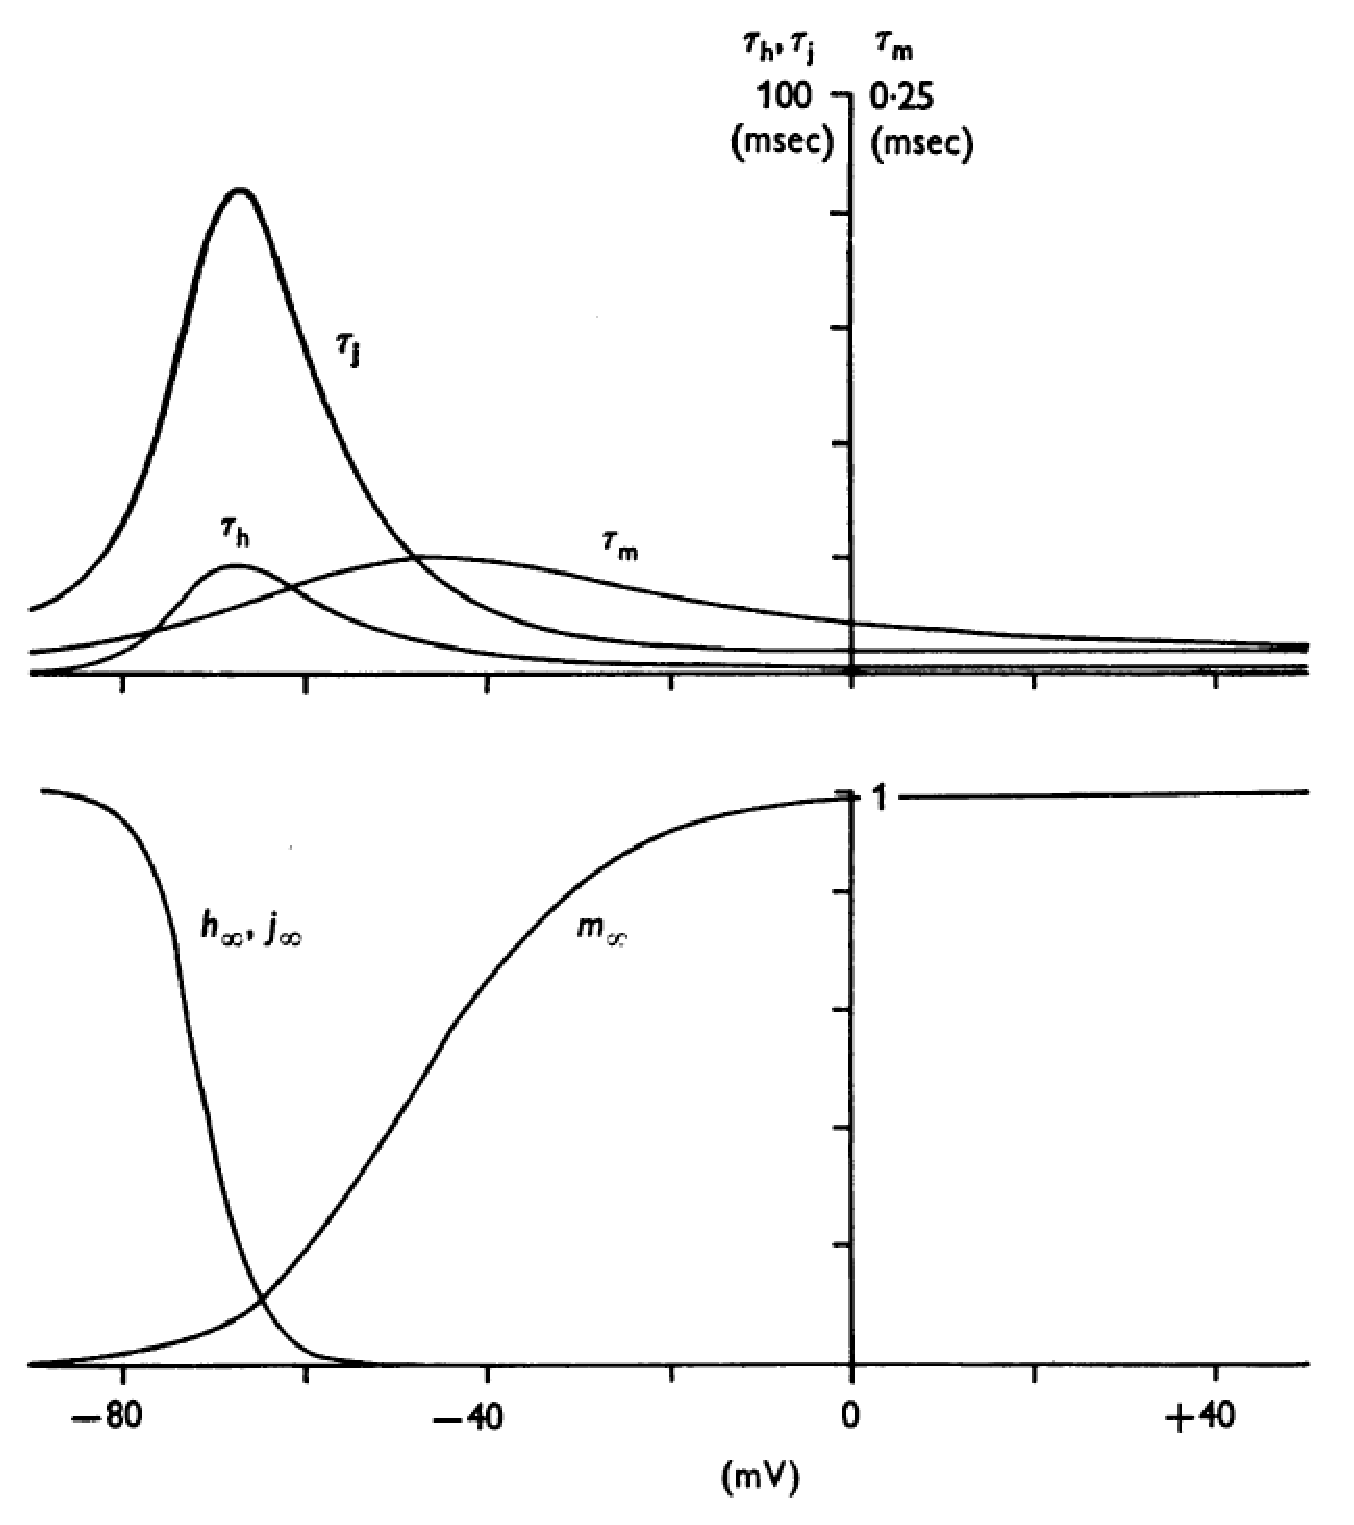
\includegraphics[height=7cm,
    angle=0]{./images/BR_mhj.eps}}
  \caption{(A) time constant, (B) steady-state values for the three
    gating variables (m,h,j) for $\Na$ current}
  \label{fig:BR_mhj}
\end{figure}

\subsubsection{$I_\na$ Sodium current}

The formula $I_\na$ is based on Hodgkin-Huxley formulation, i.e. $m$ is
activating parameter with cooperative binding number is 3 and $h$ is
inactivating parameter\footnote{h = fraction of non-inactivated channels}.
However, it is found that, in ventricular myocytes, the recovery
(re-activation)\footnote{reactivation = change of $h$ from zero back to
  unity} is much slower than the inactivation
process\footnote{inactivation = change of $h$ from 1 toward 0}. This is because
the AP duration (APD) in ventricular myocyte is longer. To account for this
longer repolarization process, Haas {\it et al.} (1971) suggested that there are
two inactivating variables. Following this idea, Beeler-Reuter introduced a second
inactivation variable $j$, eq.~\eqref{eq:85}. The dynamic of $j$ is obtained by
setting $j_\infty=h_\infty$. As shown in Fig.~\ref{fig:BR_mhj}, the steady-state
$h_\infty$, $j_\infty$ have identical dependence on membrane potential, whereas
their time constants are much different. % The time constant for these
% three parameters (m,h,j) is given in Fig.~\ref{fig:BR_mhj}.

\begin{figure}[hbt]
  \centerline{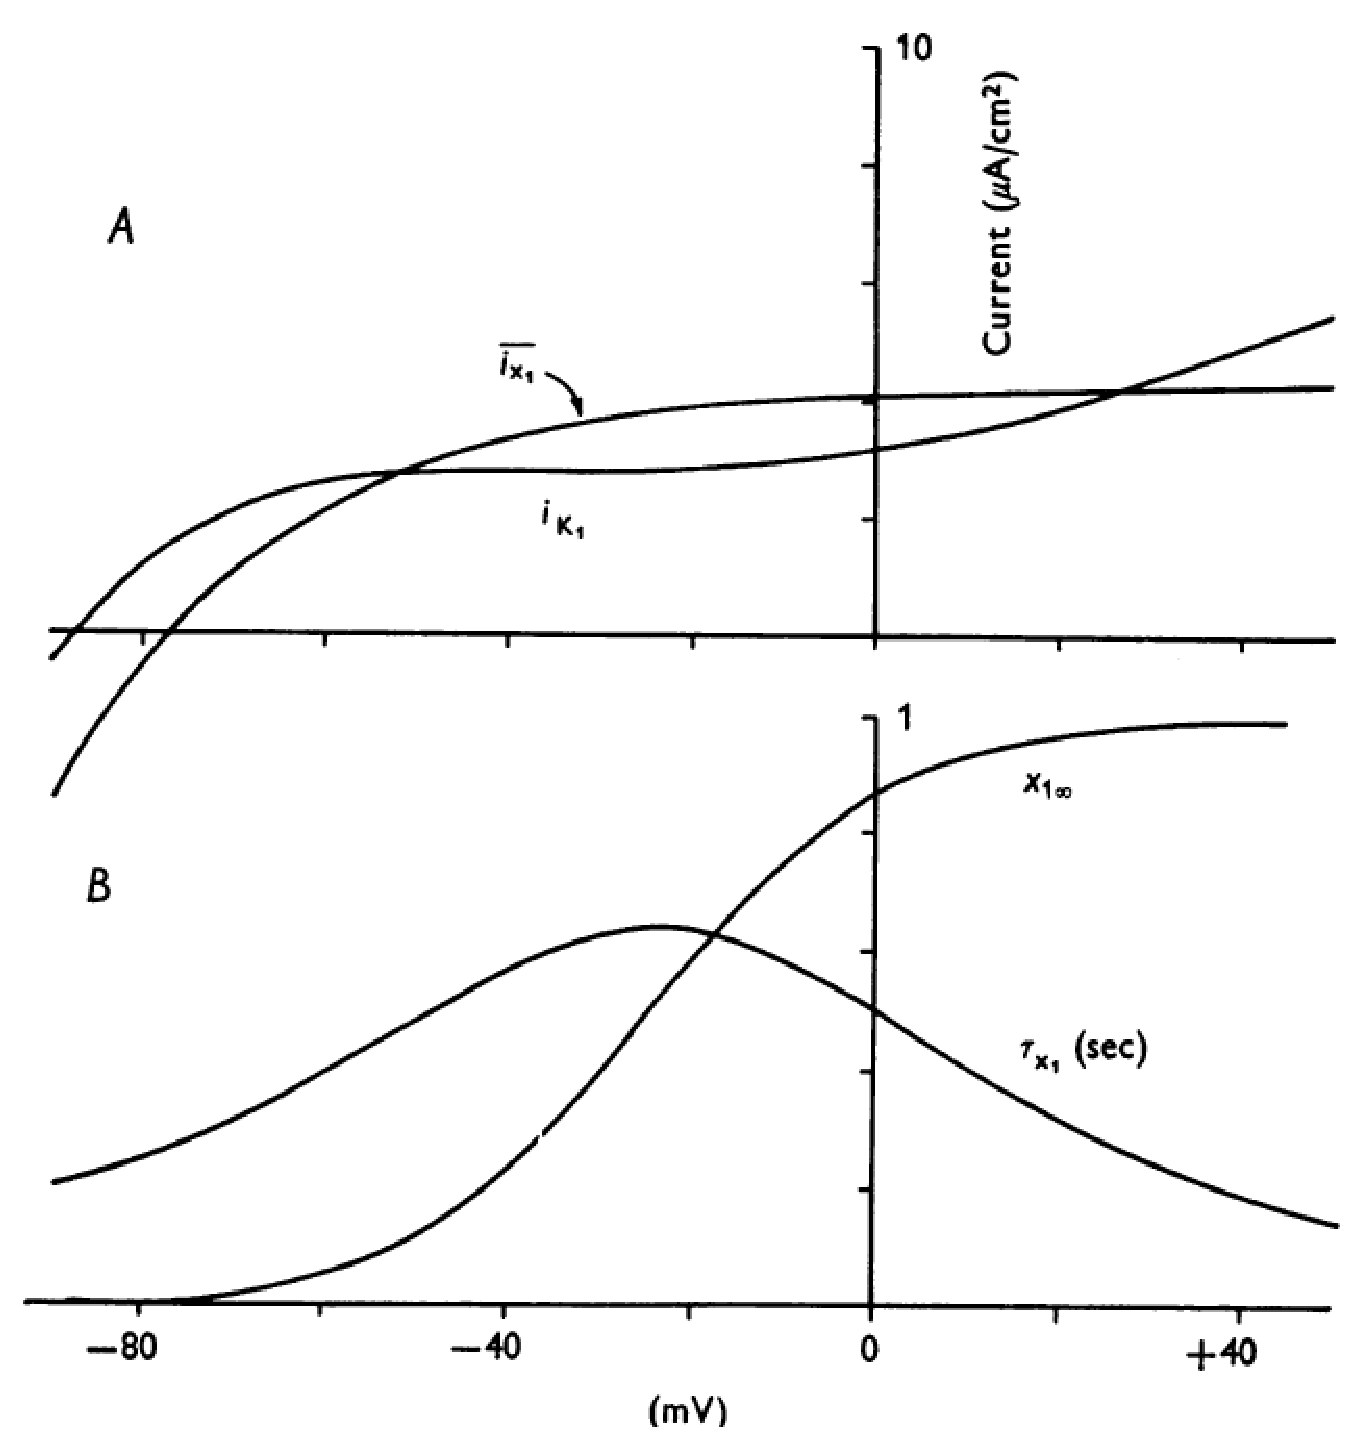
\includegraphics[height=7cm,
    angle=0]{./images/BR_ix1.eps}}
  \caption{(A) The fully activated I-V relation for $I_{x1}$ and
    background outward current $I_{K1}$; (B) steady-state value for
    the activation parameter $x_1$ and time constant $\tau_{x1}$; one
    with sigmoid shape and bell-shaped function of $V_m$, respectively}
  \label{fig:BR_ix1}
\end{figure}

\subsubsection{$I_{x1}$ Potassium current}

The kinetics of $I_{x1}$, as shown in Fig.~\ref{fig:BR_ix1}(A), is
similar to that modelled in McAllister-Noble-Tsien model and thus
inherit the formula from MNT model~\citep{mcallister1975rea}, eq.\ref{eq:618}.  

\subsubsection{$I_{K1}$ Potassium current}

The time independent outward $I_{K1}$ ($I_\Kdr$) also use the formula
from MNT model, eq.\ref{eq:619}.

\subsubsection{$I_\si$ Calcium current}

Beeler-Reuter assumed this type of channel is carried mainly by calcium, and
used a simplified eq. \eqref{eq:81}. Under that assumption, Nernst equation is
used for the resting potential of $\Ca$ channels, as given in
eq.~\eqref{eq:620}.
\textcolor{red}{This assumption is not correct} as the study of current via
$\Ca$ channel {\it per se} shown its complex behavior and unusual inactivation. It 
means that the channel permeate not only calcium, but also other ions. Later
models will use the GHK equation to find the reversal potential $E_s$
(Sect.~\ref{sec:GHK_current}).

\begin{figure}[hbt]
  \centerline{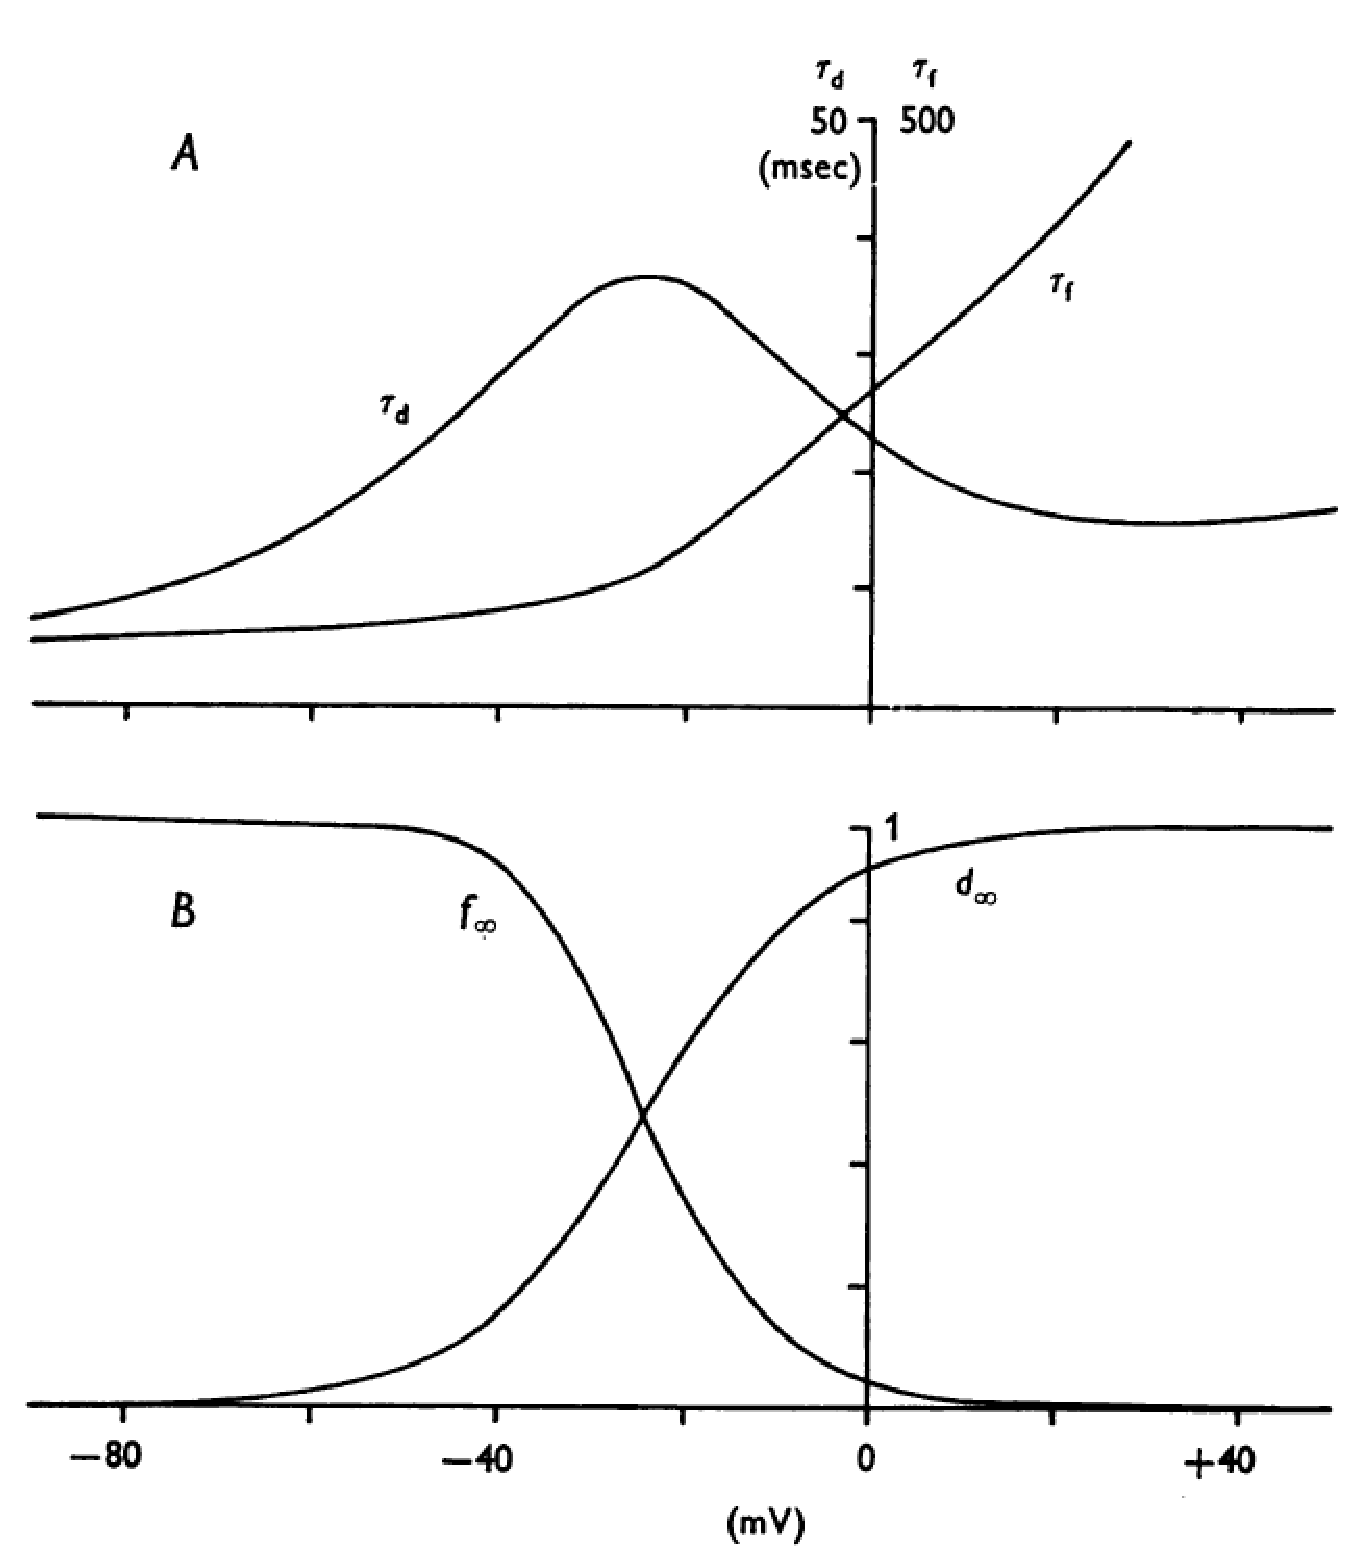
\includegraphics[height=8cm,
    angle=0]{./images/BR_df.eps}}
 \caption{(A) time constant, (B) steady-state values for
   activation/inactivation variables (d,f) of slow-inward calcium
   channels}
\label{fig:BR_df}
\end{figure}

\subsubsection{Calcium ions}


Concentration of extracellular ions on the multicellular preparations were
unknown. So, \textcolor{blue}{extracellular concentrations of ions are assumed
to  be fixed}.
The model represent a single space-clamped patch of membrane. So to model the
calcium dynamics $d[\Ca]/dt$, they assumed that the calcium flow into a small
compartment inside the cell (few percent of total cell volume) before it is
removed by an uptake mechanism which will reduce the calcium concentration in
the volume exponentially with time. The resting level of calcium in this small
compartment is $0.1\muM$ (or $10^{-7}$M), and the rate constant for the uptake
is 70 ms$^{-1}$, i.e. eq.~\eqref{eq:400}.


\subsection{Mathematical model}
\label{sec:mathematical-model-7}

The derivative of the membrane potential is given
\begin{equation}
  \label{eq:575}
  \Csc\frac{dV_m}{dt} = -\sum I_{ion} + I_{app}
\end{equation}
with $\Csc=1\mu$F/cm$^2$ closed to experimental value in literature.

Background currents
\begin{enumerate}
  \item $\Na$ background current
  \begin{equation}
  I_{\na,b} = g_{\na,b}(V_m-E_\na)
  \end{equation}
  $g_{Na,b}=0.003$ mmho/cm$^2$ (background sodium conductance, chosen
  to produce a sodium leak $0.4\mu$A/cm$^2$ at resting potential).
  
\end{enumerate}
\begin{enumerate}
\item fast inward $I_\na$ is adopted from Haas {\it et al.} (1971)
  with two inactivating variables
  \begin{equation}
    \label{eq:85}
    I_\na = (\overline{g_\na}m^3.h.j) (V_m-E_\na) 
  \end{equation}
  with $\overline{g_\na} = 4$ mmho/cm$^2$ (fully activated conductance),
  and  $E_\na = 50$ mV. The three gating variables: m (activation), and
  h,j (two inactivation).

\item The slow-inward time-dependent and voltage-dependent calcium
  current $I_\si$ is modelled in Beeler-Reuter model as follows. The
  activation and inactivation are both voltage-dependent.
  (\textcolor{red}{indeed the inactivation also depends on}
    $[\Ca ]_i$, later models have better formula)
    
  \begin{equation}
    \label{eq:81}
    I_\si = \overline{g_\si} .d .f \times (V_m-E_s)
  \end{equation}
  where $\overline{g_\si}=0.1$ (or 0.09) mmho/cm$^2$ is the maximum
  conductance of calcium ion channel; with $d(V_m,t),f(V_m,t)$ are
  activation and inactivation parameters, respectively. The kinetics
  of the gating variables $d$ was chosen to produce a time constant of
  about 22 ms at $V_m=0$ mV, and an inactivation gate $f$ with a very
  long constant (about 300 ms).

\item The reversal potential of calcium channels was assumed to be a
  function of $[\ca]_i$ only and formulated with
  \begin{equation}
    \label{eq:620}
    E_s = -82.3 - 13.0287\ln([\Ca]_{i})
  \end{equation}
  with $[\Ca]_{i}$ is the intracellular calcium concentration.
  
  For the change in intracellular calcium concentration $[\ca]_i$, a
  simplified formula was developed by assuming that
  ``{\it Ca influx first stay in a small enough volume close to the
    sarcolemma and then being uptaken to the cytosol}''.
  \begin{equation}
    \label{eq:400}
    % \frac{d[\ca]_{in}}{dt} = -10^{-4}I_\si + 0.07
    % (10^{-4}-\ce{[Ca]}_{in})
    \frac{d[\ca]_{i}}{dt} = -10^{-7}I_\si + 0.07 (10^{-7}-\ce{[Ca]}_{i})
  \end{equation}
  The parameters are based on the fact that the resting level of Ca
  concentration in the restricted space is $10^{-7}$M, and being
  reuptake with a rate constant is 70 ms$^{-1}$ (or 0.07 s$^{-1}$).

\item The outward time-dependent potassium current $I_{x1}$ is adopted
  from McAllister-Noble-Tsien model.
  \begin{equation}
    \label{eq:618}
    I_{x1} = \overline{I_{x_1}}x_1 = \frac{0.8(\exp [0.04(V_m + 77)]-
      1)}{\exp [0.04(V_m + 35)]} .x_1
  \end{equation}
with $x_1$ the gating variable. 

\item  The outward time-independent potassium current $I_{K1}$ is modelled as 
  \begin{equation}
    \label{eq:619}
    \begin{split}
      I_{K1} = 0.35\left\{\frac{4(\exp [0.04(V_m + 85)]- 1)}{(\exp
        [0.08(V_m + 53)] + \exp [0.04(V_m + 53)]) } \right.+ \\
    \left.\frac{0.2(V_m + 23)}{(1-\exp [-0.04(V_m + 23)])}\right\} 
    \end{split}
  \end{equation}


\end{enumerate}

The six gating variables follow first-order kinetics
\begin{equation}
  \label{eq:577}
  \begin{split}
    \frac{dy}{dt} &= \frac{y_\infty-y}{\tau_y} \\
    y_\infty &= \frac{\alpha_y}{\alpha_y+\beta_y} \\
    \tau_y &= \frac{1}{\alpha_y+\beta_y} 
  \end{split}
\end{equation}
The equation for $\alpha_y, \beta_y$ is estimated from experimental
data, with the general form is given in eq.~\eqref{eq:578}. The list
of estimated parameters is given in Fig.~\ref{fig:beeler_reuter_3}.

\begin{figure}[hbt]
  \centerline{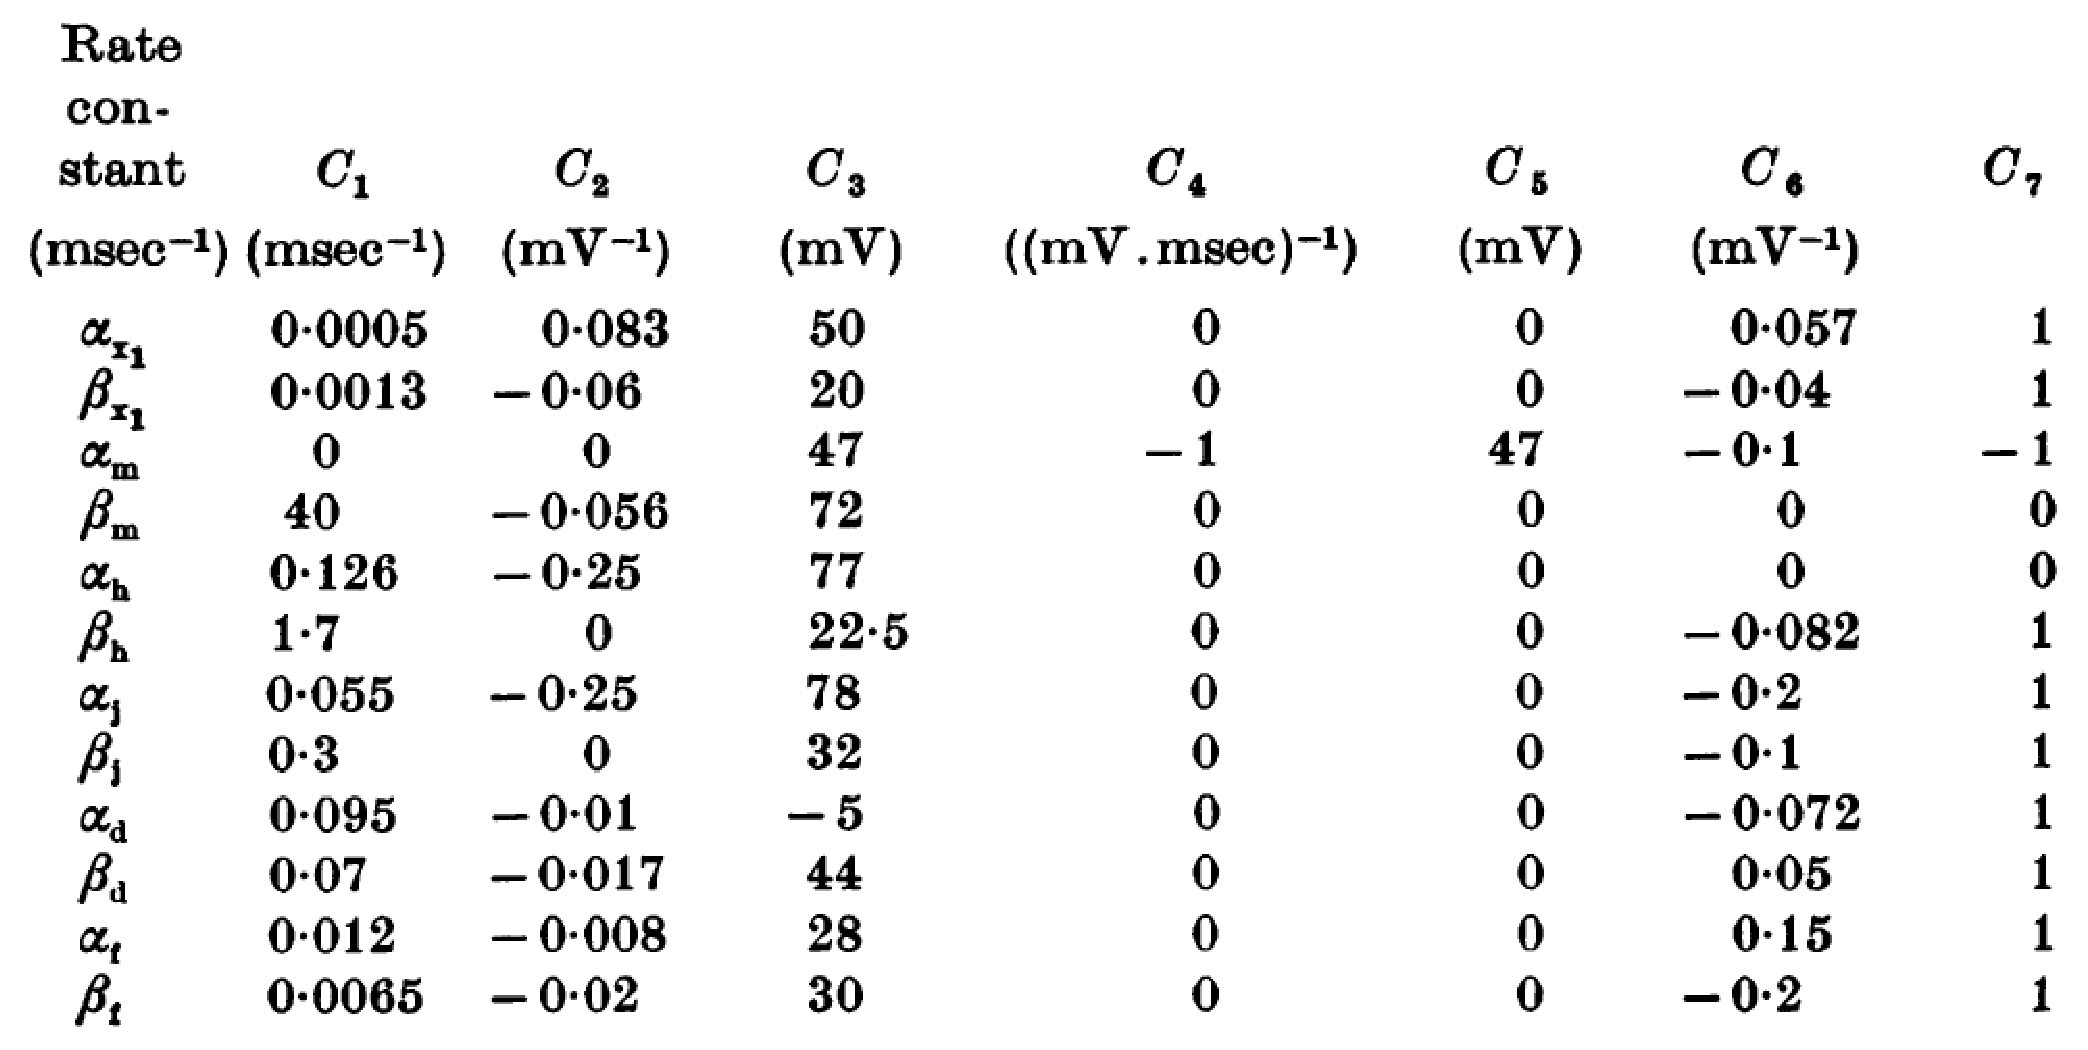
\includegraphics[height=5cm,
    angle=0]{./images/beeler_reuter_3.eps}}
  \caption{Rate constants values}
  \label{fig:beeler_reuter_3}
\end{figure}



\subsection{Units}
\label{sec:units-1}

\begin{enumerate}
\item Specific membrane capacitance: $\Csc = 1\mu F/$cm$^2$ (closed to
  experimental value in \citep{weidmann1970ect}.
\item all ionic currents densities refer to per unit area, i.e. per 1 cm$^2$.So:
unit of current ($\muA$/cm$^2$)

\item conductance (mS/cm$^2$)
\item gating variables (dimensionless)
\item potential (membrane, resting) (mV)
\item time ($t,\tau$) (msec)
\item concentration ($mole/l$ or M) 
\item rate constant ($\alpha, \beta$) (msec$^{-1}$)
\end{enumerate}
membrane potential is the difference between inside vs. outside. 


\subsection{Analysis}
\label{sec:analysis-8}

\textcolor{blue}{BR model, for the mammalian ventricular myocyte has 8
  parameters to be integrated}~\citep{reuter1973dcc, beeler1977rap}.
They are (1) membrane potential $V_m$, (2) $[\Ca ]_{i}$, (3-8)
six activation and inactivation gating parameters, e.g calcium current
(d,f), sodium current (m,h,j) and potassium current ($x_1$).

The shape of a ventricular myocyte AP can be reproduced,
Fig.~\ref{fig:BL_cardiacAP}. By stimulating a steady outward current,
the model can also produce oscillation, i.e. pace-maker activity in
Fig.~\ref{fig:beeler_reuter_2}, with the shape similar to AP of that
in SA node.
\begin{figure}[hbt]
  \centerline{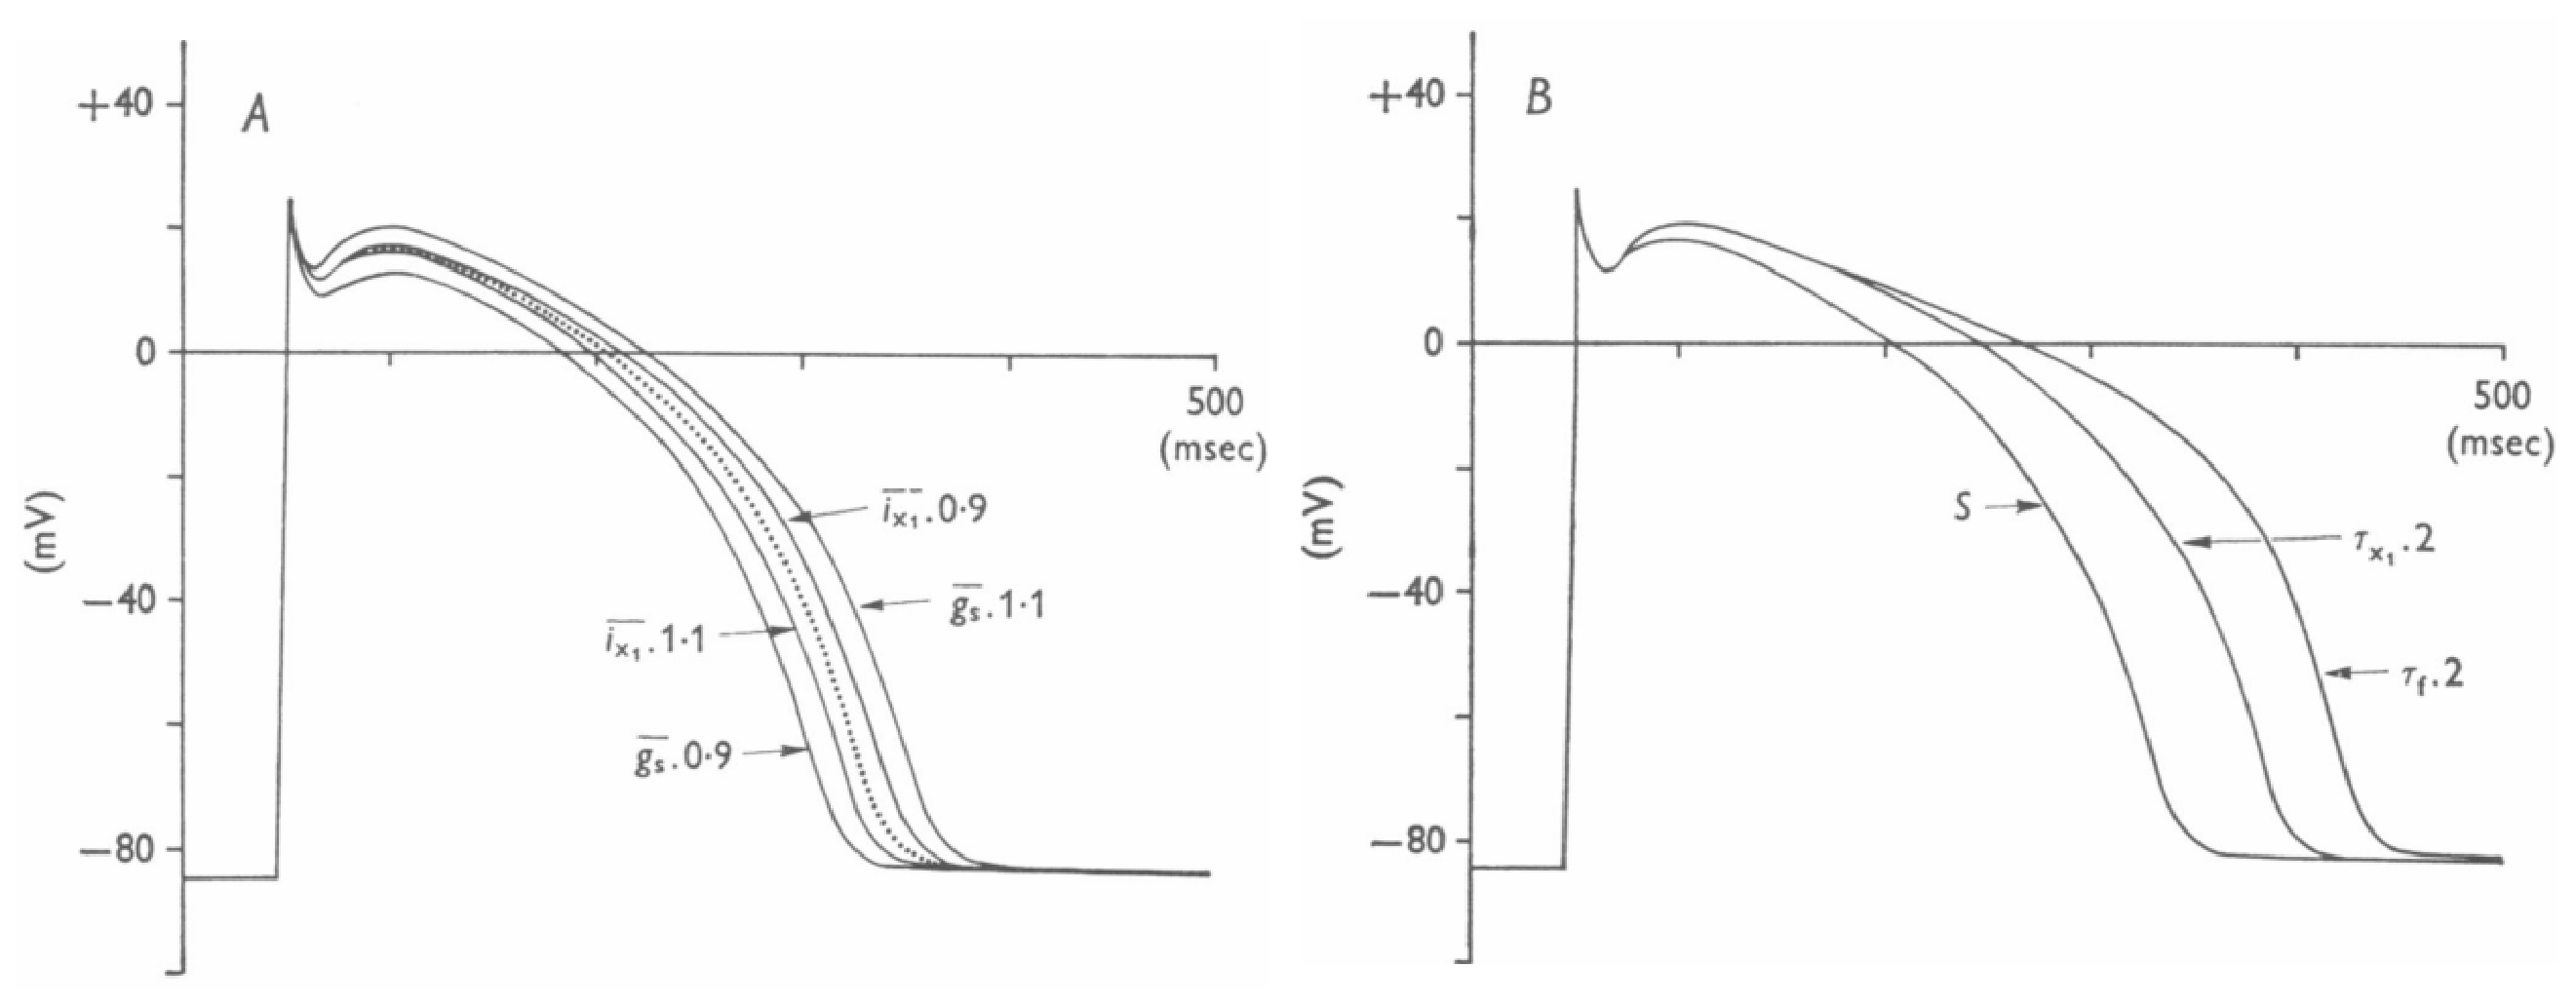
\includegraphics[height=5cm,
    angle=0]{./images/BL_cardiacAP.eps}}
  \caption{AP with varying $I_{x1},I_\si$ $\pm 10\%$; (B) increasing
    the time constant for $x_1$ and $f$ by a factor of 2 (Standard AP
    indicated by S). NOTE: increase $f$ by 2 will slowing the
    inactivation}
\label{fig:BL_cardiacAP}
\end{figure}
At a higher stimulated current, we observe a damped oscillation
(Fig.~\ref{fig:beeler_reuter_2}(B)). However, in this model, the
oscillation doesn't depend upon $g_\na$. It is indeed depending on
the slow inward current $I_\si$ (calcium). Further analysis showing
that higher $[\ca]_o$ shortening the cardiac AP (Fig. 13 paper).

\begin{figure}[!hbt]
  \centerline{    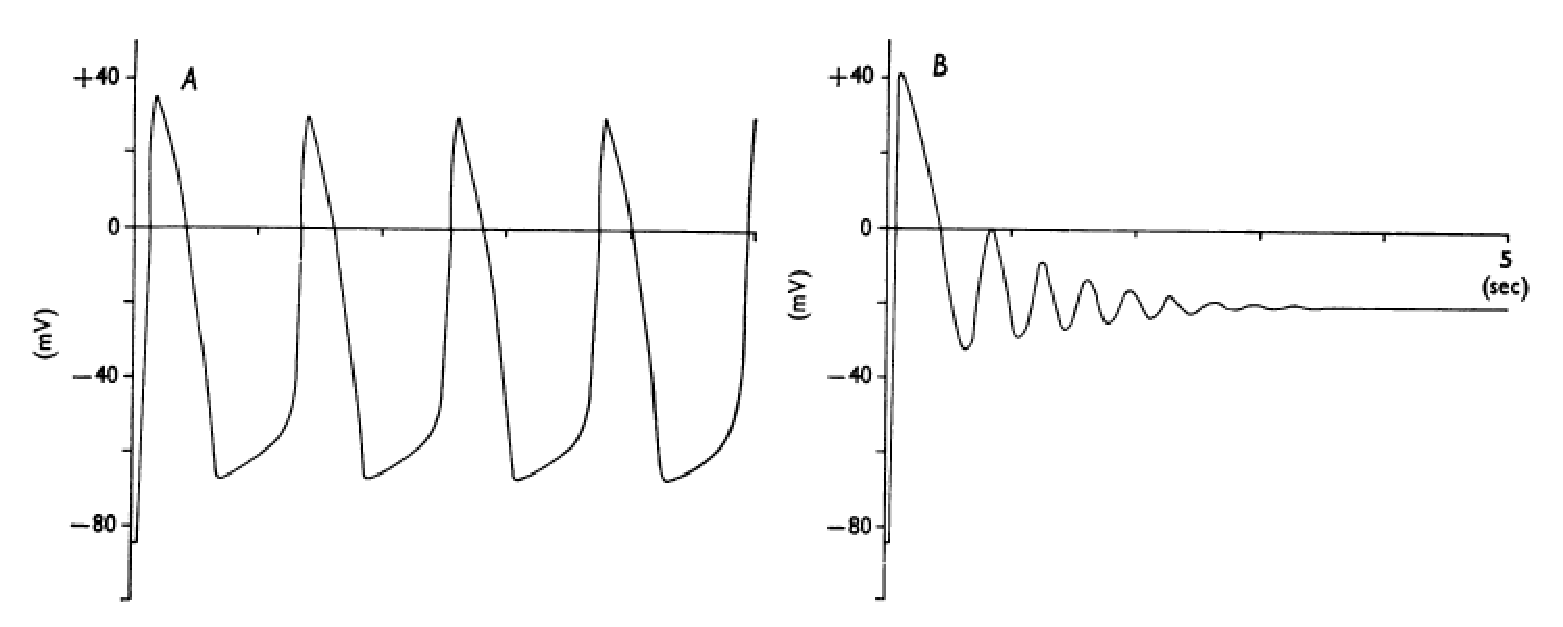
\includegraphics[height=5cm,
    angle=0]{./images/beeler_reuter_2.eps}}
    \caption{Membrane potential oscillate created with steady outward
      currents (A) 2.3$\mu$/cm$^2$, (B) 2.8$\muA$/cm$^2$}
    \label{fig:beeler_reuter_2}
\end{figure}

We study the ratio of Ca channels in each state,
Fig.~\ref{fig:beeler_reuter_1}.
\begin{figure}[!hbt]
  \begin{minipage}[b]{0.5\linewidth}
    \centering
    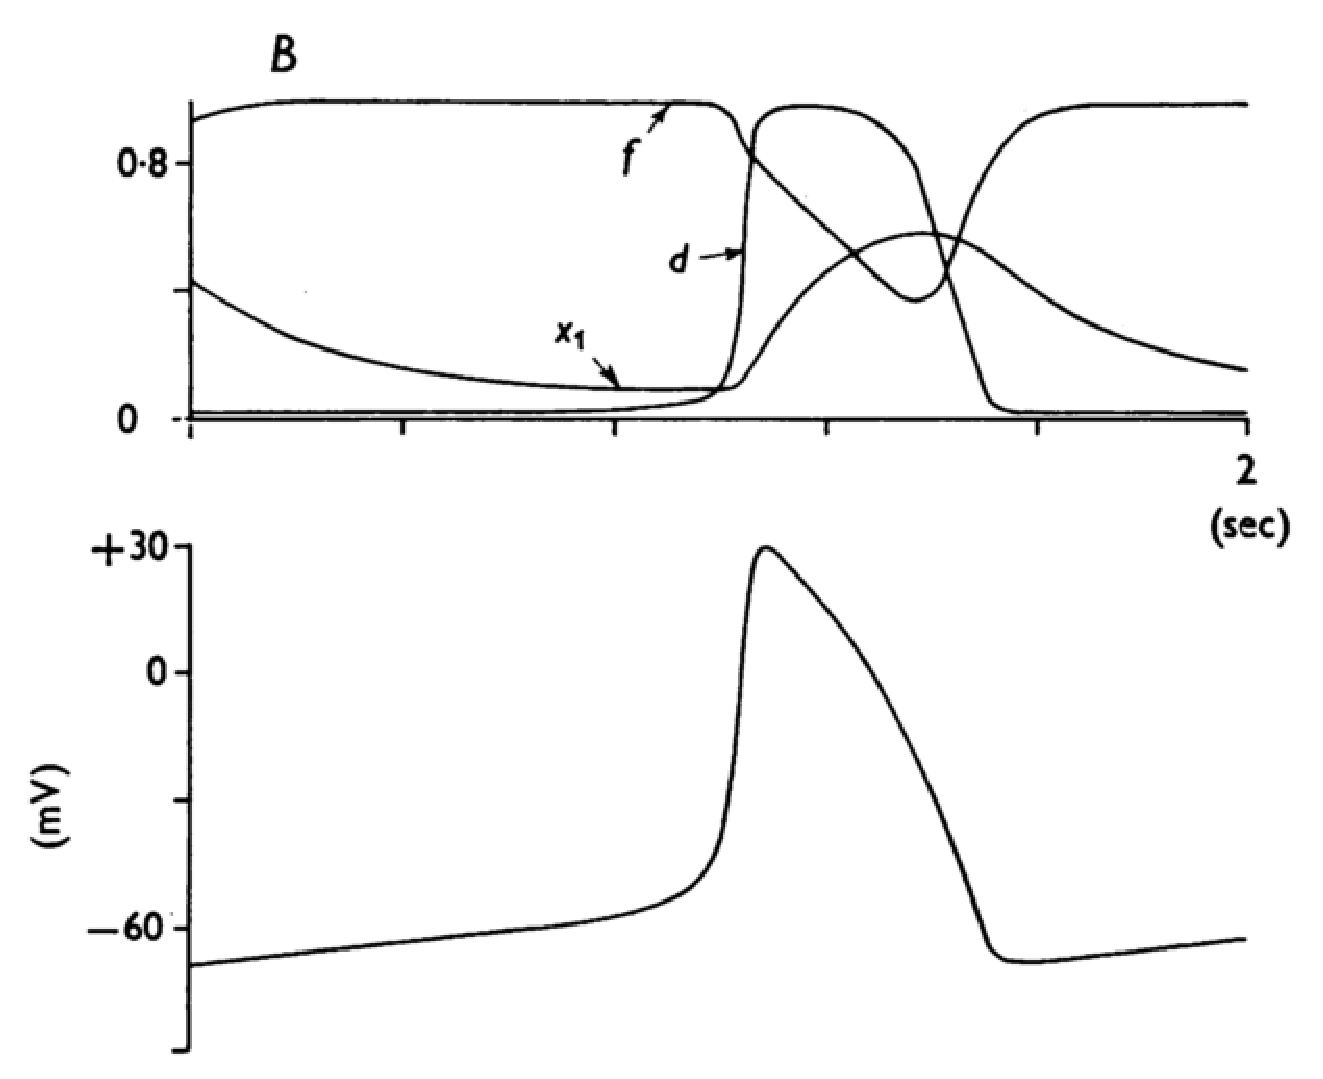
\includegraphics[height=5cm,
    angle=0]{./images/beeler_reuter_1.eps}
    \caption{The parameters values $d,f$ for $I_\si$ tell the ratio of
      Ca channels in open state ($d$) and close state ($f$)}
    \label{fig:beeler_reuter_1}
\end{minipage}
\hspace{0.5cm}
\begin{minipage}[b]{0.5\linewidth}
    \centering
  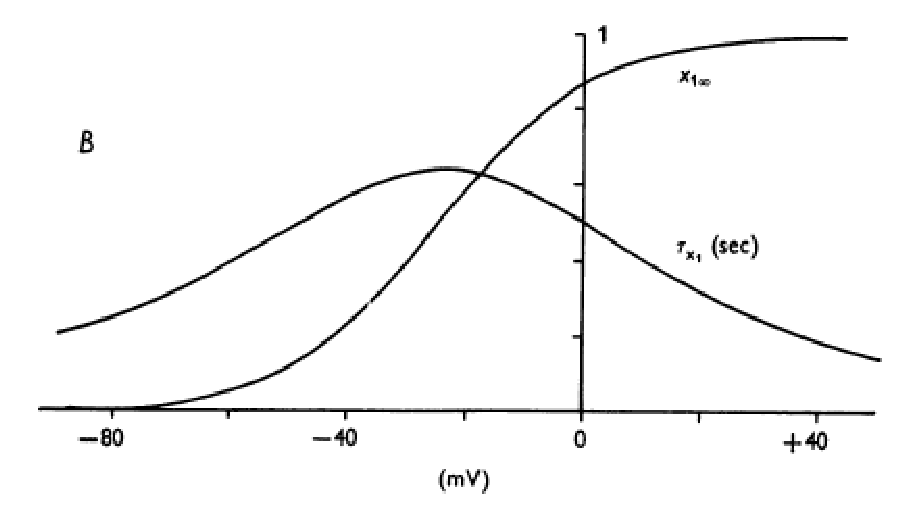
\includegraphics[height=4cm,
  angle=0]{./images/beeler_reuter_4.eps}
\caption{Steady-state value for the activation parameter $x_1$ and
  time constant $\tau_{x1}$}
\label{fig:beeler_reuter_4}
  \end{minipage}
\end{figure}

The steady-state values for the rate constant $\alpha$ and $\tau$ show
that the activation parameter $x_{1_\infty}$ has the sigmoid shape and
time constant $\tau_{x1}$ has the bell-shaped, as shown in
Fig.~\ref{fig:beeler_reuter_4}.

In this model, the value of $V_m$ has little effect on the shape of
the AP, with the sole exception of the rapid upstroke. It is the time
constants of the dynamics of ion conductances that determine the
shape.

\subsection{Numerical solution}
\label{sec:numerical-solution-2}

Using the simulation system, named Simcon, that runs on Control Data Corporation
3500 computer, they implemented the code in FORTRAN 77. The integration was
written using Runge-Kutta-Merson algorithm (Sect.\ref{sec:rkm}). 

The parameters list has 300 items, while the number of dependent variables is 8.
The maximum step size is limited by the smallest time-constant in the system
being integrated. Among the 8 dependent variables, $m$ for the activation of
sodium current has the time constant of an order faster than any other time
constants of other variables. Also, this variable is in the steady-state value
at all time except during the upstroke of the AP. So, rather than using very
small time steps at all time during the simulation, which is not necessary, an
adaptive time strategy was used. Indeed, we only need small time step during the
upstroke of AP.

To detect when upstroke of AP occur, an algorithm that monitor (1) the
difference between $m$ and its steady-state value, (2) instantaneous rate of
change of membrane potential ($dV_m/dt$). If (1) the difference is less than
0.004, and (2) $dV_m/dt < 0.5$ (V/sec), then steady-state approximation of $m$
can be used. Otherwise, $dt$ is chosen smaller, and the ODE for $m$ is used.
NOTE: This strategy enhanced the performance 20x in speed, i.e. a single AP was
computed in about 40sec.

The value of $m$ in the last integration step is kept to check for the
rate of change of $m$. The rate of change is
\begin{equation}
  \label{eq:574}
  \text{rate} = \frac{\text{stead-state value - m in last integration}}{dt}
\end{equation}
If this rate exceed 0.005/sec, then the integration of  $m$ is
computed again. 

There are three modes of simulation:
\begin{enumerate}
\item mode 1:(most common - deterministic) give a set of initial
  conditions and proceed through a subsequent set of integration step
  to find the time evolution of the $V_m$. Then, we plot I-V
  curves. 

\item mode 2 (Voltage-clamp): simulate an ideal voltage-clamp experiment, i.e.
set the membrane potential $V_m$ from the resting potential to the desired
voltage-clamp $V_{step}$. In this mode, only one ODE is used, as the only
depenent variable to $V_m$ to study is $[\Ca ]_i$, while gating parameters can
be expressed as an exponential function and need not be integrated.

\item mode 3: similar to the voltage-clamp experiment, with the
  external applied current varies via the formula
  \begin{eqnarray}
    \label{eq:401}
    I_{app} = I_{clamp} = \frac{V_{clamp} - E_m}{R_s}
  \end{eqnarray}
  with $R_s$ is the series resistance (e.g. $R_s = 200\Omega$), $E_m$ is the
  potential across the membrane patch. 
\end{enumerate}
\textcolor{red}{Data presented in the paper mainly used the third method.}


\subsection{Conclusion}
\label{sec:conclusion} 

The model is deterministic. The membrane AP is based on two inward
($I_\si,I_\na$) and two outward currents ($I_{K2},I_{x1}$). The model can
reconstruct the shape of AP, i.e. the prolonged plateau of AP. However, it lacks
the predictability, e.g. during conduction or conduction disturbance (e.g.
arrhythmias).

In addition, the model behavior is an ``all-or-none'' repolarization. In 1975,
the mechanism relating Calcium elevation to excitation-contraction in the cell -
calcium-induced calcium-release (CICR) - was discovered by
~\citep{fabiato1975cic} in which Calcium was released from a main Calcium
internal storage - SR. This model has not incorporated this. Another issue is
that CICR is a regenerative process, and thus leading to a paradox of control,
as graded elevation of global calcium was observed. A new hypothesis - known as
{\bf local control theory} - was proposed in 1992~\citep{stern1992tec} with
$\Ca$ sparks as elementary events which as observed by~\citep{cheng1993cse}
using confocal microfluorimetry.

The kinetics of the dynamic currents are far from completion at this
time, especially $I_\na$. This model belong to the class of the
so-called ``common pool'' model in which the behavior is considered as
the ensemble average of all ion channels in the whole cell, i.e.
\textcolor{blue}{uniform distribution}. 

\begin{enumerate}
\item The effect of the change in extracellular ion concentration had
  not been considered.
\item no electrogenic pump has been considered
\item cannot predict AP during conduction or conduction disturbance
  (arrhythmias). 
\end{enumerate}
Nowadays, $I_\si$ is known as the net current through (1) two types
of calcium channels (long-lasting L-type and transient
T-type)~\citep{bristow1982mmp}, (2) $\ce{Na+}/\Ca $ exchangers, (3)
some miscellaneous background currents.

This calcium inactivation in this model is assumed to be
voltage-dependent only. However, later experimental results shown a
calcium-mediated inactivate the calcium current
also. Standen-Stanfield model (Sect.~\ref{sec:standen_1982model}) was
the first to recognize this. So, in many ways, BR model is not
accurate, yet still a good starting point.

\begin{framed}
  Using {\it constant field theory}~\citep{pickard1976gghk}
  (Sect.~\ref{sec:GHK_voltage}), the calcium current is estimated
  using GHK equation
  \begin{equation}
    \label{eq:360}
    \begin{split}
      % I_\ca = P_\ca\frac{z_\ca^2V_mF^2}{RT} \left[ \frac{[\ca]_i-[\ca]_o\exp(z_\caV_mF/RT)}{1-\exp(z_\caV_mF/RT)}\right] +\\
      I_\si = P_\ca \frac{z_\ca ^2V_mF^2}{RT} \left[ 
      \frac{\gamma_{Ca,o}[\ca]_o-\gamma_{Ca,i}[\ca]_i\exp(z_\ca V_mF/RT)}{1-\exp(z_\ca V_mF/RT)}\right] +\\
      \sum_X P_X \frac{z_{X}^2V_mF^2}{RT} \left[
        \frac{\gamma_{X,o}[X]_o-\gamma_{X,i}[X]_i\exp(z_{X}V_mF/RT)}{1-\exp(z_{X}V_mF/RT)}\right]
    \end{split}
  \end{equation}
  with the second term on the right-hand side is the sum of contribution
  from sodium and potassium ions through the channels.
  \begin{itemize}
  \item $z_\ca =2$ [unitless]
  \item $V_m=$ membrane potential [mV]
  \item $F=$ (Faraday constant) [C/mol] or [mJ/(mV.mol)]
  \item $X$ is \ce{Na+} and \ce{K+}, then $z_X = 1$
  \item $P_X$ is the permeability of ion X [cm/sec]
  \end{itemize}
  This is a more accurate and widely used on later models. 
\end{framed}

\section[Standen-Stanfield model (1982)]{Standen-Stanfield model (frog atrial
  myocyte) (1982)}
\label{sec:standen_1982model}

\begin{figure}[hbt]
  \centerline{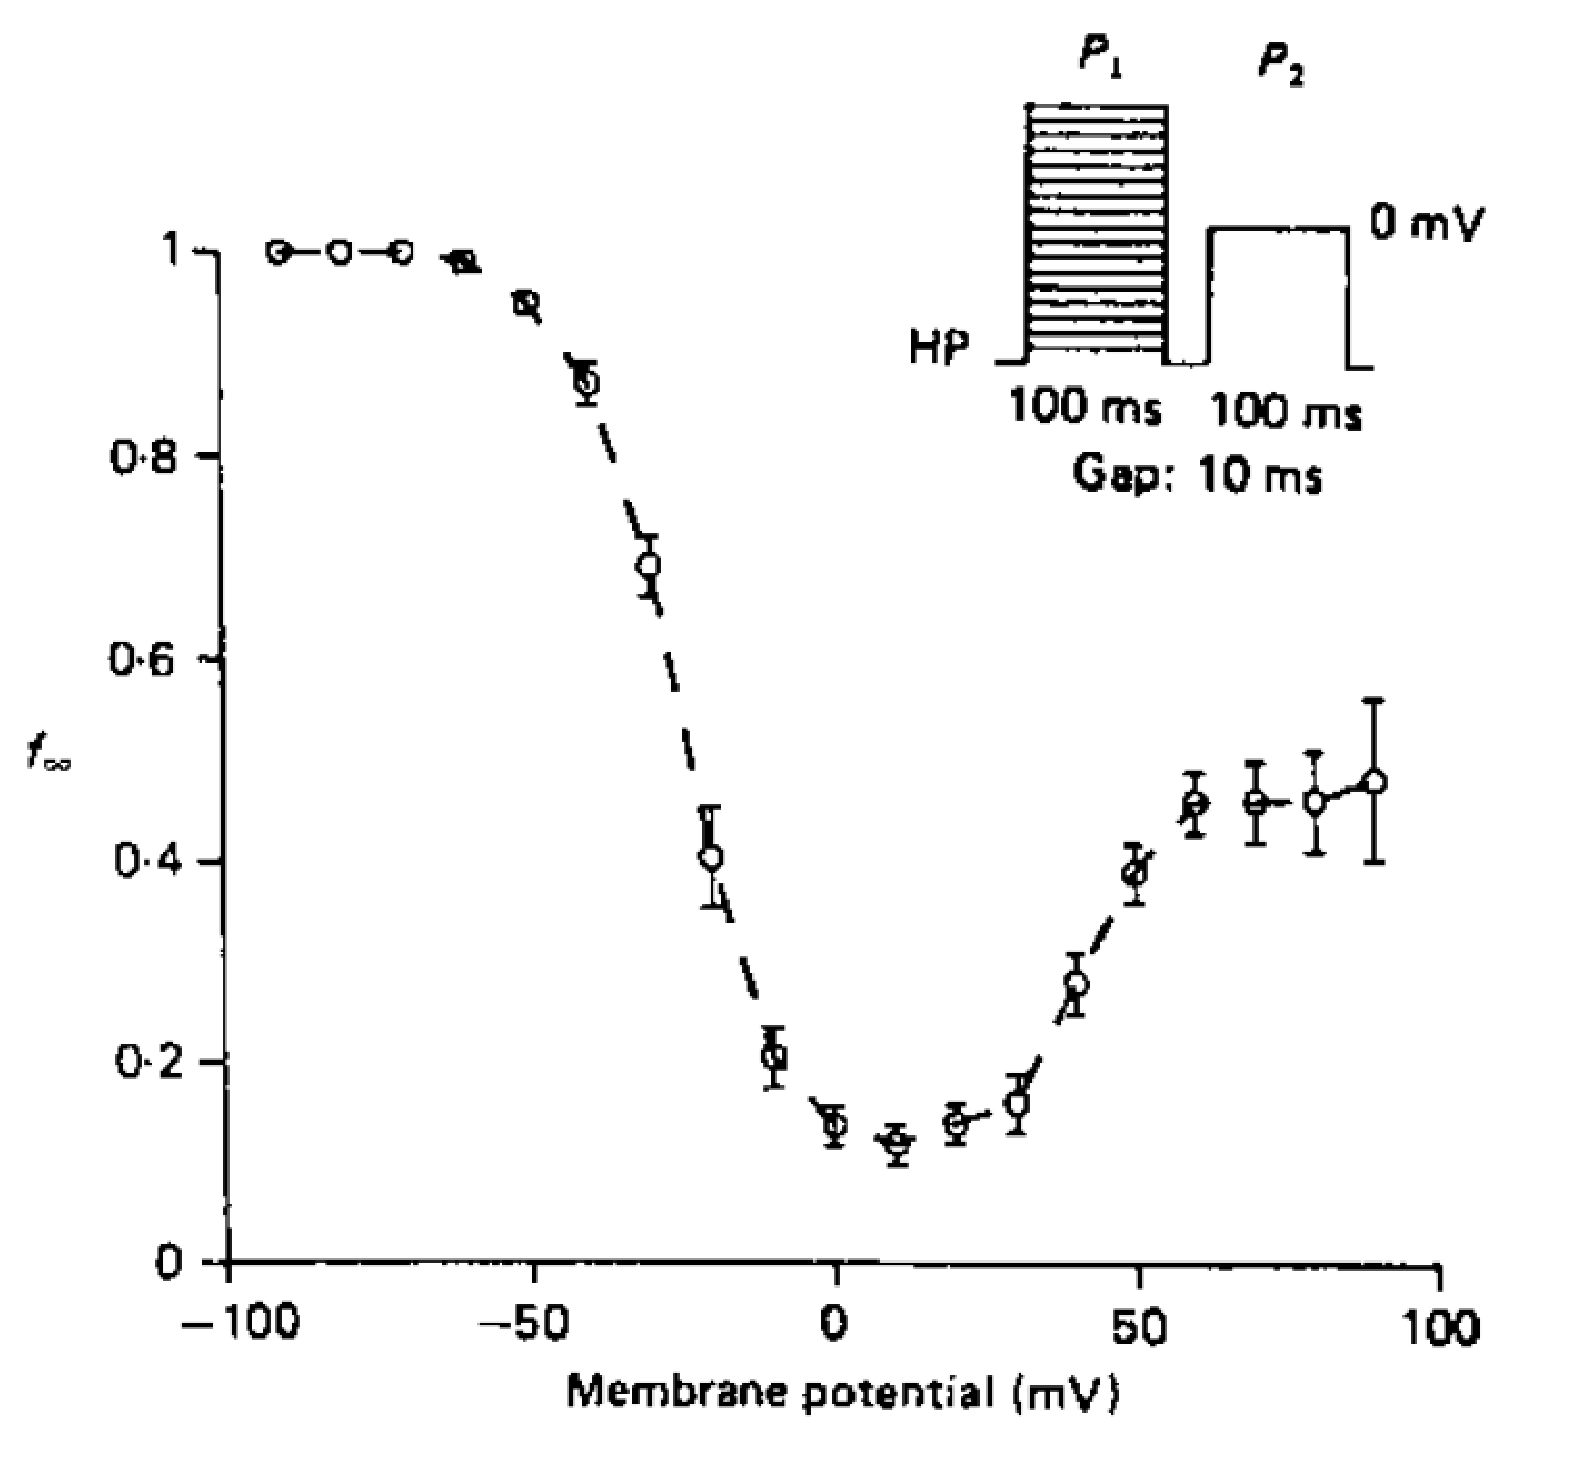
\includegraphics[height=7cm,
    angle=0]{./images/Ca_inactivation.eps}}
  \caption{Steady-state fraction of closed channels $f_\infty$ at different
  membrane potential $V_m$ (mV) in frog atrial myocytes}
  \label{fig:Ca_inactivation}
\end{figure}

So far, computational models assumed $V_m$-dependent only on activation and
inactivation of calcium channels.  In Fig.~\ref{fig:Ca_inactivation}, the
inactivation increase in accordance to the increase of membrane voltage until
$V_m=20mV$, from that we observe a decrease in inactivation, i.e. more channels
to open, until the steady value 0.45. However, the HH-based model for $\Ca$
current cannot reproduce this type of inactivation. With new experimental
result, there are also strong evidence of $[\Ca]$ inactivation dependent of
calcium channels\footnote{even though \ce{Sr+} and \ce{Ba^2+} also permeate Ca
  channels, the inactivation by these ions is much lower than with $\Ca$},
  rather than membrane potential {\it per se}. 
  
 ~\citep{standen1982bsm} take this information and build a model for frog
 ventricular cells. \textcolor{red}{Standen-Stanfield model is the first one to
 propose a formula for Ca channel inactivation}. The model also consider the
 effect of buffering on $\Ca$; yet ignored all other ionic channels.
 
As the $\Ca$-dependent inactivation requires a much high level of $\Ca$
  than the bulk cytoplasmic calcium. So, they modeled this by assuming a
  submembrane region where see a much higher level of calcium the inner side
  of the cell, denoted as $[\Ca]_c$.
  Now, the inactivation is dependent upon both by $V_m$ and $[\Ca]_c$ where
  $[\Ca]_c$ is the calcium concentration in the subcompartmental area and is
  typically higher than the myoplasmic calcium concentration.

\subsection{hypothesis analysis}
\label{sec:hypothesis-analysis-3}


Similar to B-L model (Sect.~\ref{sec:beeler-reuter-model}), there was
no data for structure of the submembrane compartment. It was made
simple that this is a subvolume whose size is of fraction $\sigma$ of
the cell volume
(\textcolor{red}{in later models, with new experimental data, we will
  know that there are many small, local subspace called dyadic
  subspace} that serve as a local, temporary compartment for $\Ca$
  entry).
\textcolor{blue}{Then, it is assumed that calcium entry
  accumulating in a submembrane compartment is sequestrated by
  Ca-binding sites of buffers},
retaining a certain fraction of $\Ca$ free to diffuse into the
myoplasm and to bind to the binding site R in the $\Ca$ channels.

\subsubsection{$\Ca$ buffering}
\label{sec:buffering}


Calcium buffering is a complex process with several different
affinities. The widely assumptions are
\textcolor{blue}{(1) single binding, and (2) the rapidly buffered,
  with a very large number of binding sites}.
Then, the buffering is estimated by Michaelis-Menten equilibrium
\begin{equation}
  \label{eq:719}
  \Ca + B \ce{<=>[K_b]} \ce{CaB}
\end{equation}
with $K_b=k^+/k^-$ is the binding constant. Under the assumption of
rapid equilibrium,
\begin{equation}
  \label{eq:1044}
  \ce{[Ca][B]K_b = [CaB]}
\end{equation}
or
\begin{equation}
  \label{eq:1045}
  \ce{[Ca] = \frac{[\CaB]}{[B]K_b}}
\end{equation}
This amount of unbound $\Ca$ in the bulk myoplasm is assumed to be constant, say
$a$.

\textcolor{red}{The concentration of free Ca in this sub-compartment
  is denoted as} $[\Ca]_c$, i.e.
\begin{equation}
  \label{eq:1251}
  \ce{[Ca]_c = \frac{[\CaB]}{[B]K_b}}
\end{equation}

\subsubsection{$\Ca$ diffusion}
\label{sec:diffusion}


Calcium entry from the compartment also being removed to the cytoplasm
due to diffusion, with a rate assumed to be proportional to the
current subcompartmental calcium concentration
\begin{equation}
  \label{eq:625}
  k_s[\ca]_c
\end{equation}
However, when there is no Ca entry, the concentration of $[\ca]_c$
need to be keep at a certain level. This minimum level is called
resting level, denoted as $[\ca]_{c,r}$. To model this, it is assumed
that there is a constant leak
\begin{equation}
  \label{eq:626}
  k_s[\ca]_{c,r}
\end{equation}
of calcium back into the
sub-compartment\footnote{ this leak doesn't change with changes in
  [Ca]}.

\subsubsection{$\Ca$ channel inactivation}
\label{sec:inactivation-1}

In addition to $V_m$-dependent inactivation, the inactivation is due
to the binding of these free calcium ions in the sub-compartment to one site in
$\Ca$ channels. The binding of calcium to an intracellular binding site R is
given as follows~\citep{ashcroft1982cis}. NOTE: The channel with CaR is inhibited from
opening.
\begin{equation}
  \label{eq:382}
  % \Ca + R \ce{<=>[K_h][\beta]} CaR
  \Ca +  \ce{R <=>[\alpha(\text{$[\Ca]_c$})][\beta] CaR}
\end{equation}
with $\alpha, \beta$ are voltage-independent coefficients. The forward rate
constant is calcium-dependent while the backward one is not. 

\begin{figure}[hbt]
  \centerline{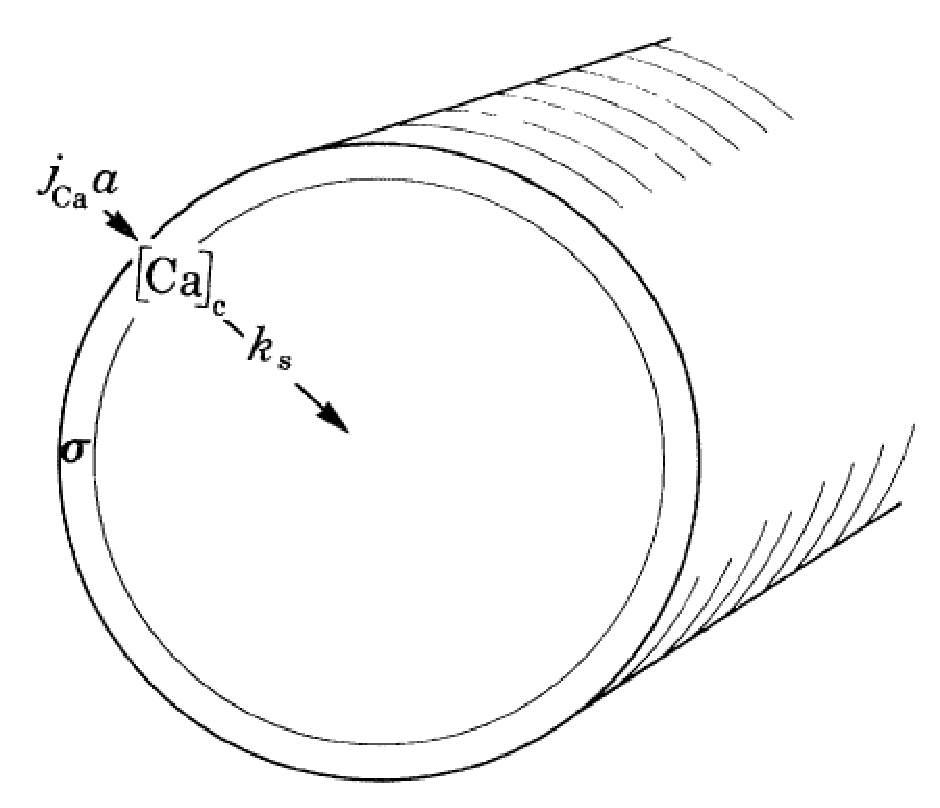
\includegraphics[height=5cm,
    angle=0]{./images/SS_sigma.eps}}
  \caption{The schematic diagram of the change in [Ca] in the
    sub-compartment}
  \label{fig:sub-compartment}
\end{figure}


\subsubsection{$\Ca$ channel currents}

Standen-Stanfield consider the fact that multiple ions can permeate through
$\Ca$ channels. So, Standen-Stanfield used {\it constant field theory}, i.e. the
general form in eq.~\eqref{eq:360}. However, they assumed that the potassium and
sodium ions have no effect on the activation of calcium current. Thus,
the approximation for the activation is given in eq.~\eqref{eq:621}.

\subsection{Mathematical model}
\label{sec:mathematical-model-8}

\subsubsection{$I_\ca$ current}
\label{sec:activation}

\begin{framed}
  Except at very positive $V_m$, the quantity
  $[\ca]_i\exp(z_\ca V_m\frac{F}{RT})$ has a very small effect on
  $I_\ca $. Thus, it can be excluded from the calculation.
\end{framed}

\begin{equation}
  \label{eq:621}
  \begin{split}
    I_\ca  = P_\ca \frac{z_\ca ^2V_mF^2}{RT} \left[
     \frac{ \gamma_{o}[\ca]_o-\gamma_{i}[\ca]_i\exp(z_\ca V_mF/RT)}{1-\exp(z_\ca V_mF/RT)}\right]
  \end{split}
\end{equation}
with $z_\ca =2$, $\gamma_o=\gamma_i=1$. $P_\ca $ is the calcium
permeability [cm/sec] whose magnitude is dependent on the
compartmental calcium concentration $[\Ca]_c$ and membrane potential
$V_m$ as given follows
\begin{equation}
  \label{eq:622}
  P_\ca =\overline{P_\ca } .m^3.h
\end{equation}
$\overline{P_\ca }=6.10^{-5}$ cm/sec~\citep{ashcroft1982cis}; $m,h$
[unitless] follow the first-order kinetics,
i.e. $dm/dt=\alpha_m(1-m)-\beta_m.m$.  The rate constants are
calculated from empirical expression~\citep{ashcroft1982cis}.
\begin{equation}
  \label{eq:623}
  \begin{split}
    \alpha_m = \frac{0.013(V_m+20)}{1-\exp(\frac{V_m+20}{3})}\\
    \beta_m = 0.031\exp(\frac{V_m+20}{25})
  \end{split}
\end{equation}
and $h$ is the inactivating variable which depends on free Ca in the
sub-compartment)
\begin{equation}
  \label{eq:1252}
  dh/dt = \alpha_h(1-h)-\beta_h [\ca]_c h
\end{equation}


However, under fast-binding assumption, a simpler formula is utilized
\begin{equation}
  \label{eq:624}
  h = \frac{K_h}{[\ca]_c+K_h}
\end{equation}
with $K_h$ is the half-saturation constant, and $h$ is considered as
the fraction of channels open.

\begin{framed}
  If the binding of calcium is assumed to be rapid, eq.~\eqref{eq:382}
  can be treated as instantaneous.  Thus, Michaelis-Menten equilibrium
  is utilized, i.e. the dissociation constant $K_h=\frac{\beta}{\alpha}$
  as the binding constant, then the fraction of open channel
  is% \footnote{the original paper use $h$ notation, here we use $f_\ca $}
  \begin{equation}
    \label{eq:630}
    % f_\ca  = \frac{K_h}{K_h +  [\ca]_c} 
    f_R = h = \frac{K_h}{K_h +  [\ca]_c} 
  \end{equation}
  with $[\ca]_c$ is the concentration of free $\Ca$ in the
  submembrane compartment; $f_R+f_{\ce{CaR}} = 1$.

  Another viewpoint is to express in term of rate of inactivation
  (\textcolor{blue}{this is not being used in the model})
  \begin{equation}
    \label{eq:383}
    % \frac{df_\ca }{dt} = \beta(1-f_\ca ) - \alpha . f_\ca  [\ca]_c
    \frac{dh}{dt} = \beta_h.(1-h) - \alpha_h . h [\ca]_c
  \end{equation}
\end{framed}



\subsubsection{$[\ca]_c$ change}
%\label{sec:ca_c-change}


As shown in Fig.~\ref{fig:sub-compartment}, the change in calcium
concentration $[\ca]_c$ in the submembrane region is caused by (1)
the diffusion to the cytoplasm, (2) the leak back into the submembrane
region, (3) and the influx of calcium across the calcium channels,
modelled as
\begin{equation}
  \label{eq:629}
  \frac{d[\ca]_c}{dt} = -k_s[\ca]_c +k_s[\ca]_{c,r} - j_\ca .\frac{a}{2F\sigma}
\end{equation}
with $k_s = 0.001$ ms$^{-1}$; $j_\ca $ (C.sec$^{-1}$.cm$^{-3}$) is the
flow of charge per unit volume of fibre (derived from $I_\Ca$ using
eq.~\eqref{eq:621} with the fibre diameter of
70$\mu$m)\footnote{the mean fibre diameter in muscle is 71.3$\mu$m};
the volume fraction of fibre that compose the submembrane compartment
$\sigma=0.2$ , and the free calcium is $a=0.05$.
\textcolor{red}{NOTE: We use the negative sign in the last term as the
  influx current of calcium has negative sign}, i.e. $j_\ca < 0$.

\begin{figure}[hbt]
  \centerline{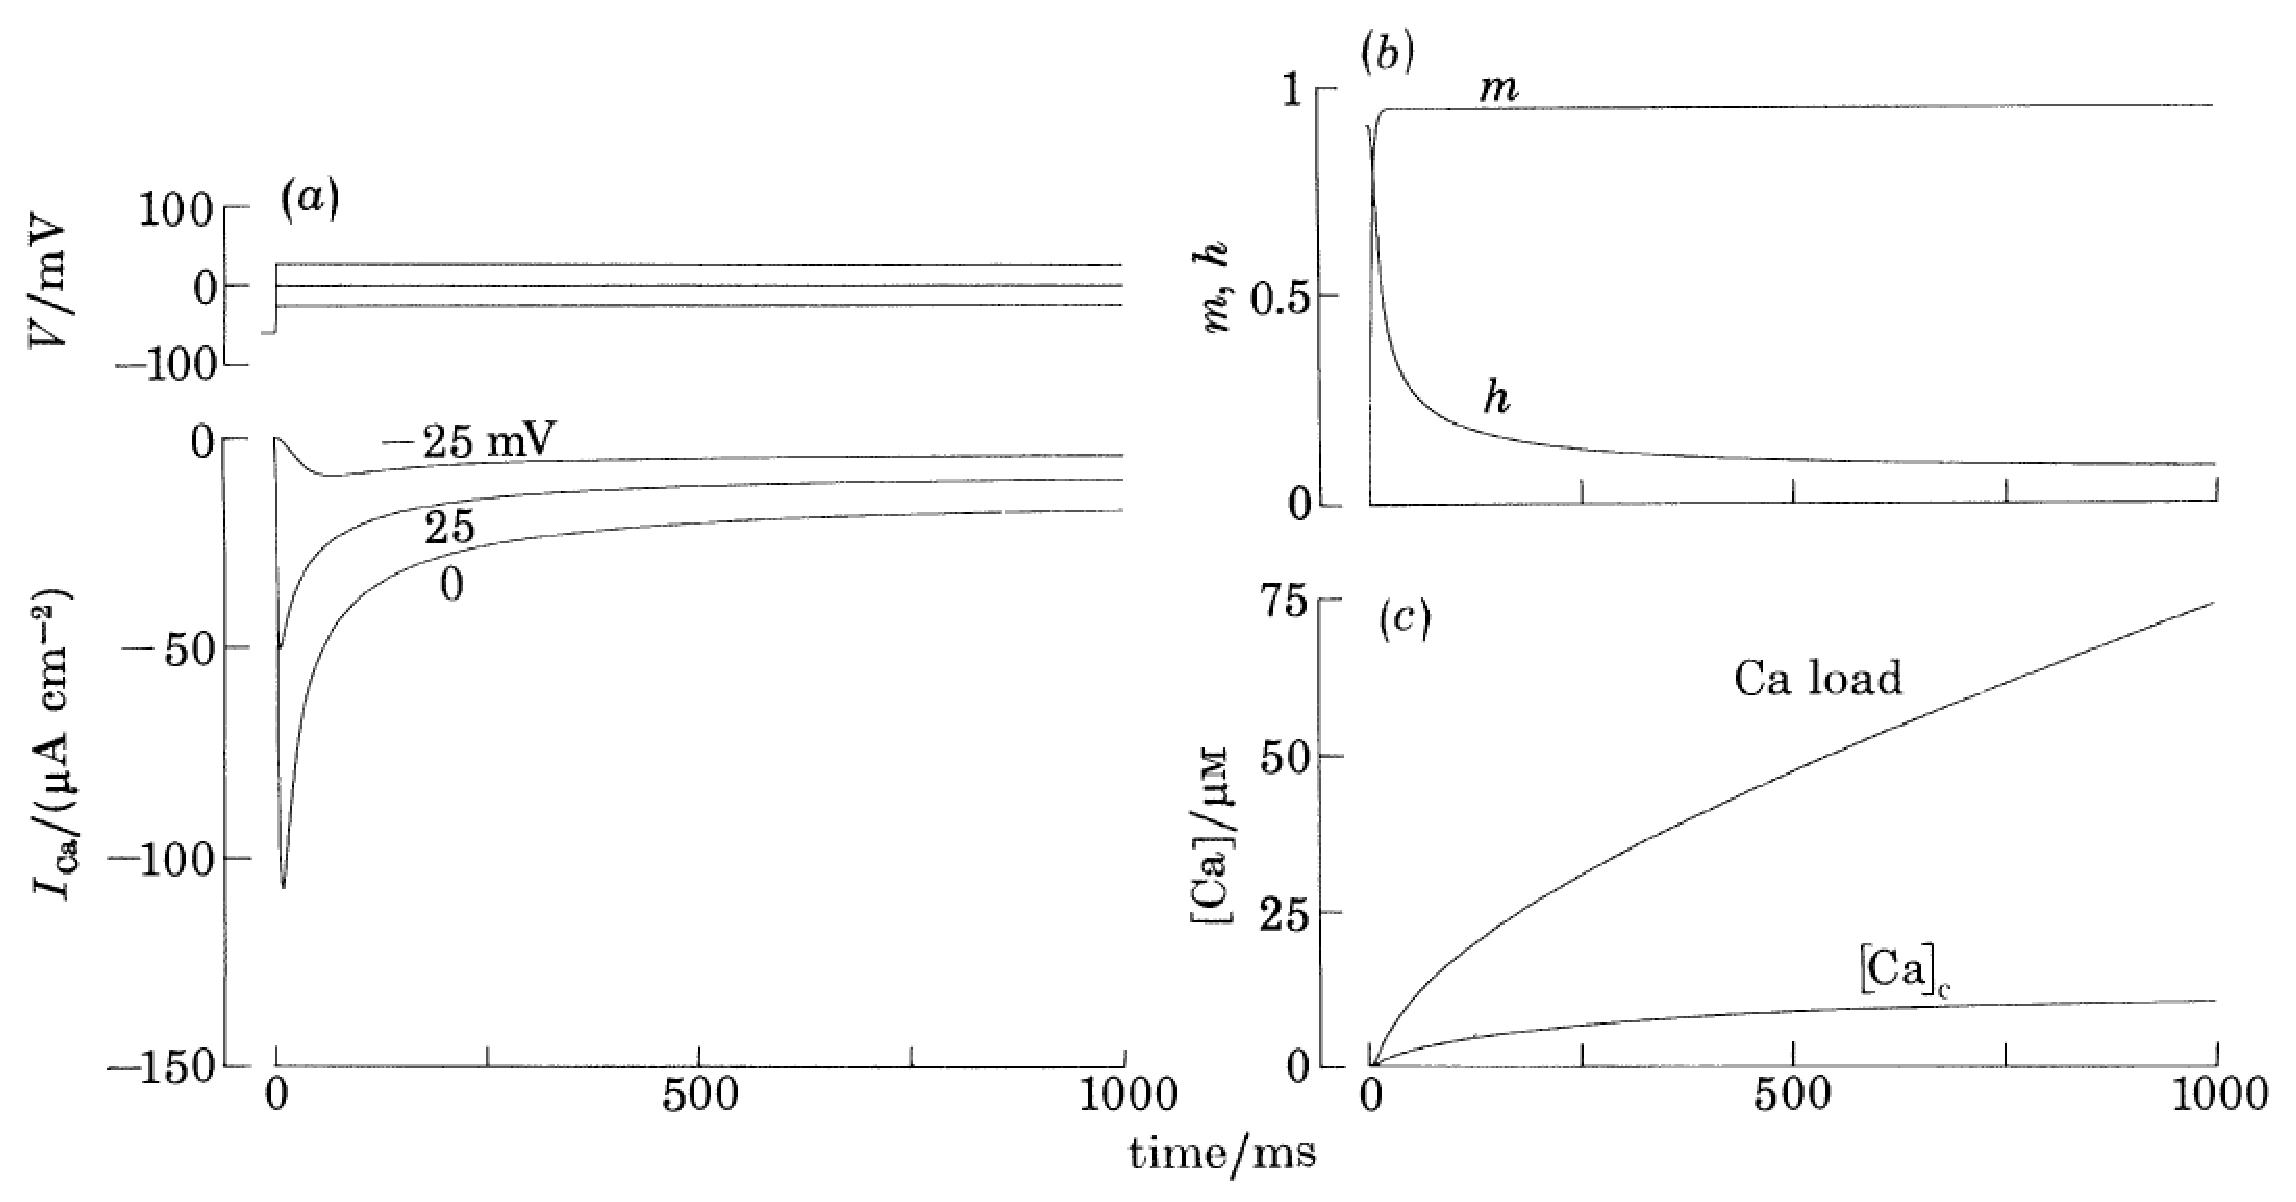
\includegraphics[height=5cm,
    angle=0]{./images/SS_calcium.eps}}
  \caption{(a) $I_\ca $ with voltage-clamp at -25mV, 0mV, +25mV from the
    holding potential -60mV. (b) the change in $m,h$ with a 1s pulse to
    0mV; (c) total $\Ca$ load entering the fibre and the rise in $[\Ca]_c$
    during the pulse in (b). \textcolor{red}{NOTE: LCC current density measured
    here is very high, not accurate. Look for newer experiments}}
  \label{fig:SS_Calcium}
\end{figure}

\begin{framed}
  REMEMBER: The membrane current per unit volume is
  \begin{equation}
    \label{eq:1040}
    j_m = 2\frac{(V_2-V_1)}{3l^2R_i} \;\;\;\text{(A/cm$^3$)}
  \end{equation}
\end{framed}

\subsection{Numerical solution}
\label{sec:numerical-solution-3}

The model was solved using {\bf Runge-Kutta} method
(Sect.\ref{sec:runge-kutta-method}) with a step size, $\Delta t = 1$ms.

\subsection{Analysis}
\label{sec:analysis-6}


REMEMBER: Besides a number of assumptions we have mentioned, the binding is also
assumed with cooperative binding number $\eta=1$. The general form is
\begin{equation}
  \label{eq:627}
  \ce{Ca^2+ + R <=>[k^+\ce{[\ca]^\eta}][k^-] Ca^2+R}
\end{equation}
at which the new gating variable will be
\begin{equation}
  \label{eq:945}
  h = \frac{(K_{m,Ca})^\eta}{(K_{m,Ca})^\eta +
    \left([\Ca]_c\right)^\eta} = \frac{1}{1 + \left(\frac{[\Ca]_c}{K_{m,Ca}}\right)^\eta}
\end{equation}
By changing the parameters ($K_h$...), we study the affect of the
Ca-dependent inactivation.

This model is still deterministic model, in which the reaction are
determined by the concentrations and rate constants, and there is no
probability element that tell how likely a reaction to occur. 

\textcolor{red}{To avoid the variations in cell geometry, in this
  model, all ionic currents are computed based on} 1.0 cm$^2$ of membrane so
  that they can be adapted to other cell types easier. \textcolor{red}{Thus, the
  specific membrane capacitance} is set at $\Csc=1\mu$F/cm$^2$. This is the
  standard that will be used in all modern computational models.

\section{Luo-Rudy Phase I (1991) - ventricular cardiac cells}
\label{sec:luo-rudy-phase-1}

With new experimental data (using single-cell single-channel recording),
~\citep{luo1991mcap} developed a model for a general ventricular cardiac cells -
not targetting to any particular species, namely Luo-Rudy phase 1 (LR-1) model.

\textcolor{red}{Units of ionic currents here is} $[\mu$A/cm$^2$]. Units
of gating variables are [1/ms]. 

\subsection{Hypothesis analysis}
\label{sec:hypothesis-analysis-2}

HH model measure data at $T=6.3^\circ$C. In this model, the data were
adjusted to 37$^0$C using a Q$_{10}$ adjustment factor
(Sect.~\ref{sec:q10-factor}).
\begin{itemize}
\item Compared to the B-R model (Sect.~\ref{sec:beeler-reuter-model}),
  $I_{K1}$ (or $I_{K,DR}$) now becomes 3
  distinct currents $I_{K1},I_{Kp},I_b$). The equivalent of $I_{K1}$ in B-R
  model is $I_{K1(T)}$ which is the total time-independent potassium current
  \begin{equation}
  I_{K1(T)} = I_{K1} + I_{Kp} + I_b
  \end{equation}  

\item  LR-1 has 6 ionic currents. 

\item Compared to DiFrancesco-Noble model, LR-1 has not incorporated
  any ionic pumps or exchange (available in LR-phase 2 -
  Sect.~\ref{sec:luo-rudy-phase-2}).
\end{itemize}

\subsubsection{$\Ca$ concentrations}

Similar to B.R. model, as the simulation was short-enough, all ionic
concentrations were assumed to be fixed, except $[\ca]_i$. The
values chosen for ion concentrations are: $[\ce{K}]_o=5.4$mM,
$[\ce{K}]_i=145$mM, $[\Na]_i=18$mM, $[\Na]_o=140$mM, and
$[\ca]_o=1.8$mM. The initial value for cytoplasmic calcium
concentration is $[\ca]_i=2\times 10^{-4}$mM. The dynamic of the
calcium concentration was given in eq.~\eqref{eq:740}.

\subsubsection{Na currents}
\label{sec:ionic-currents-1}

For the fast sodium current $I_\na$, LR-1 model inherited the
activation $m$ and inactivation $h$ gating variable from E-J
model\footnote{fit data from cardiac cell (chick-embryo) with
  realistic rate of depolarization $\dot{V}_{max}=300$mV/sec}
~\citep{ebihara1980fsc} (Sect.\ref{sec:Ina_E-J-model}). Also, to model the slow
recovery, the $j$ inactivation gating variable from B-L model was added
(Sect.\ref{sec:Ina_Beeler-Reuter_1977}), eq.~\eqref{eq:724}. 

\subsubsection{$\Ca$ current}

For the slow-inward current $I_\si$, RL-1 utilized the B-L model's
formula, i.e. the activation and inactivation are purely
Voltage-dependent. Thus, there are two gating variables $d$
(activation) and $f$ (inactivation), eq.~\eqref{eq:386}.
\textcolor{red}{The role calcium-inactivation that has been proposed
  in Standen-Stanfield model was not considered here}.
As a result, $I_\si$ in this model is still not correct; RL-2 fixes
this (Sect.~\ref{sec:luo-rudy-phase-2}).

\begin{figure}[hbt]
  \centerline{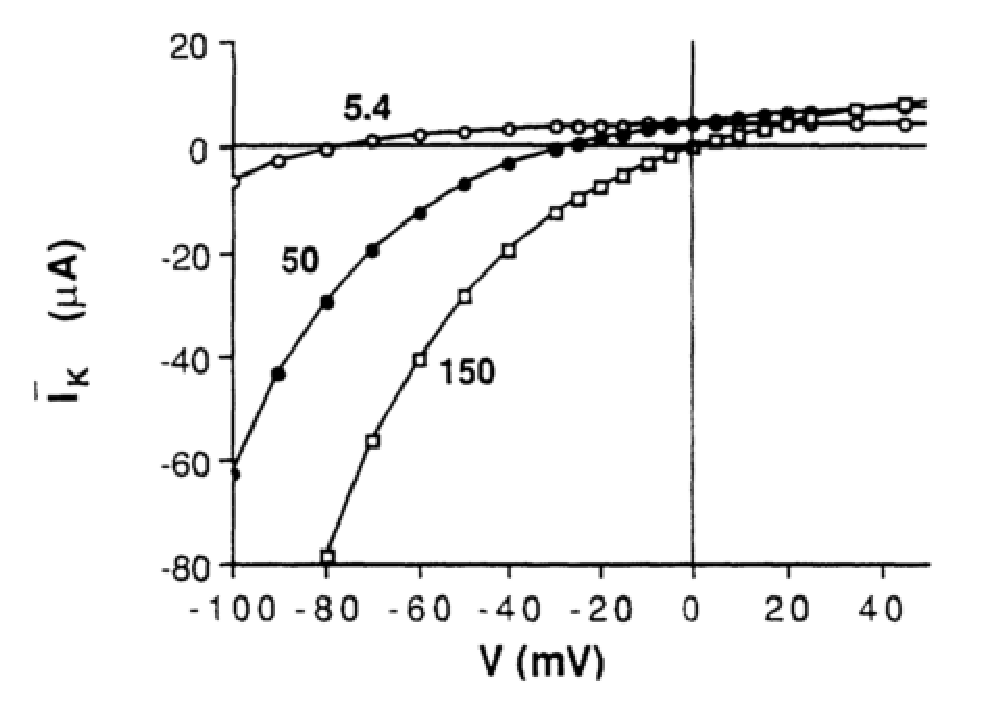
\includegraphics[height=5cm,
    angle=0]{./images/LR1_IK.eps}}
\caption{I-V curve of fully activated $\overline{I}_K$ for $[\K]_o$=5.4, 50 and
150 mM}
\label{fig:LR1_IK}
\end{figure}

\subsubsection{$\K$ time-dependent current}

The hyperpolarizing-activated inward current $I_f$ in
DiFrancesco-Noble model and $I_{x1}$ in B-L model is now denoted as
$I_\k$, eq.~\eqref{eq:628}. The kinetics was based on result obtained
from nodal cells of rabbit heart~\citep{shibasaki1987ckd}, with two
gating variables $X$ (time-dependent activation) and $X_i$
(time-independent inactivation).  Shibasaki also claimed that the
kinetics of this current was not altered by $[\ce{K}]_o$; but the
single-channel conductance is proportional to $\sqrt{[\ce{K}]_o}$,
eq.~\eqref{eq:746} and eq.~\eqref{eq:747}. The parameters was fitted
based on Fig.~\ref{fig:LR1_IK}.

\subsubsection{$\K$ time-independent current}

In RL-phase1 model, the definition of $I_{K1}$ differs from that in
B-R model and in MNT model, i.e. B-R $I_{K1}$ (when the knowledge of different
potassium channels had not been discovered) is equivalent to $I_{K1(T)}$
\begin{equation}
  \label{eq:1046}
  I_{K1(T)} = I_{K1}+I_{Kp} + I_b
\end{equation}
So, $I_{K1}$ in RL-1 is just a component. 

\begin{enumerate}
\item The time-independent $K1$ current, eq.~\eqref{eq:720}.

\item In 1988, Yue-Marban discovered a new potassium current,
  activating at the plateau range, from guinea-pig ventricular heart
  cells, and quite selective to $\ce{K+}$ ions~\citep{yue1988ncp}. Due
  to its high active at plateau range, it was given the name $Kp$.
  The ``plateau'' $Kp$ current, eq.~\eqref{eq:721}.

\item Also, Kurachi found that $K1$ has an inactivation gate which
  depends upon both $V_m$ and $E_{K1}$~\citep{kurachi1985vdc}. 
\item To account for the non-specific background current, they denoted it as
$I_b$, eq.~\eqref{eq:722}.
\end{enumerate}

The parameters were fitted using data in Fig.~\ref{fig:LR1_IK1T}. 

\begin{figure}[hbt]
  \centerline{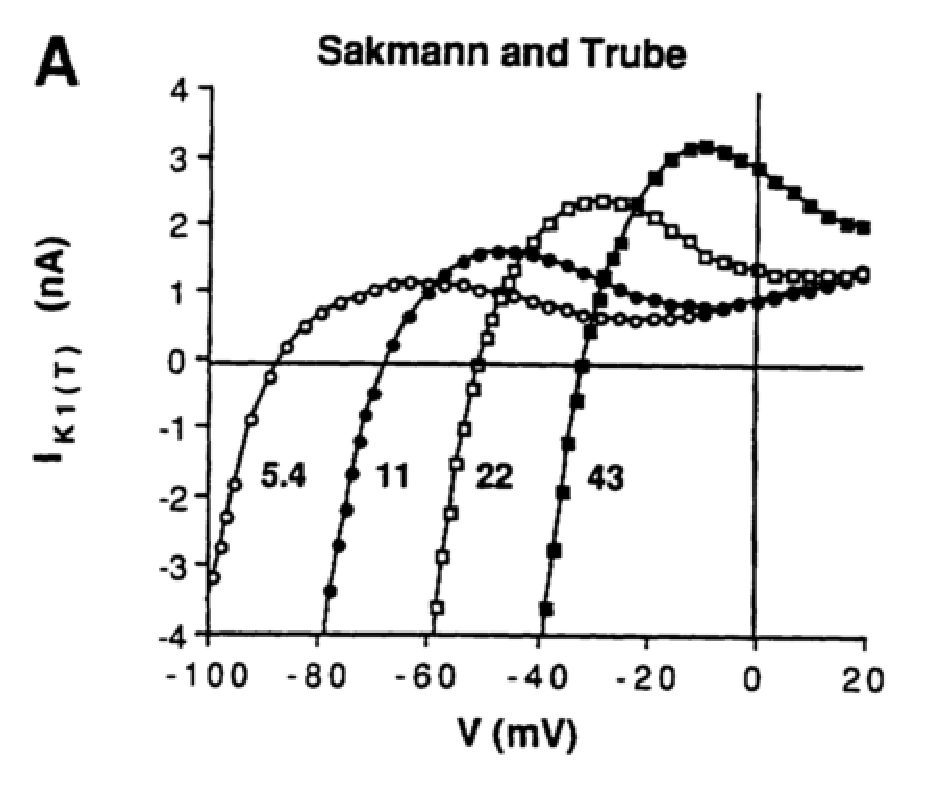
\includegraphics[height=5cm,
    angle=0]{./images/ST_IK1T.eps}, 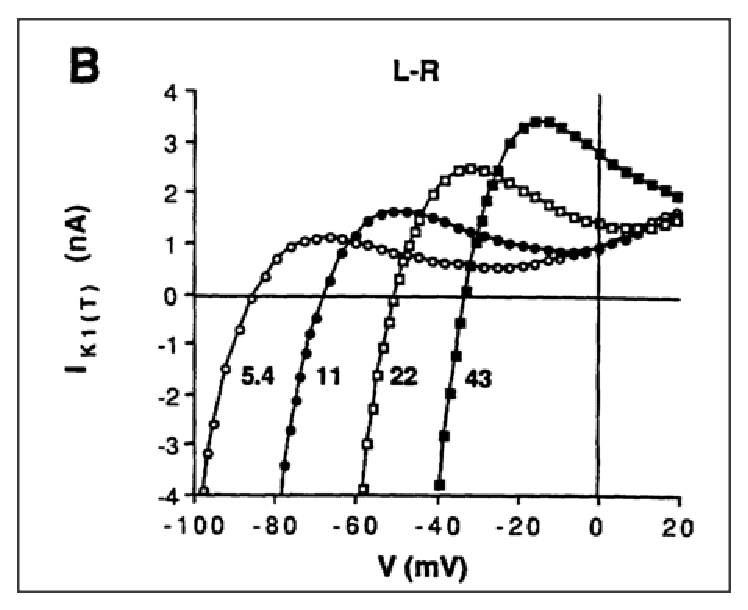
\includegraphics[height=5cm,
    angle=0]{./images/LR1_IK1T.eps}}
\caption{Sakmann and Trube experimental data; LR-1 simulation result}
\label{fig:LR1_IK1T}
\end{figure}

% The total time-independent potassium current is
% $I_{K1(T)}=I_{K1}+I_{Kp}+I_b$. 


% Again, Standen-Stanfield formulation is the basis for the model (read
% Sect.~\ref{sec:standen_1982model}). Yet Luo-Rudy squared the
% concentration term to increase the steepness of the relation between
% intracellular calcium and inactivation.
% \begin{equation}
%   \label{eq:385}
%   f_\ca  = \frac{1}{1 + ([\Ca]_i/K_m)^2}
% \end{equation}
% with $K_m$ is the calcium concentration that produce half-maximal
% calcium inactivation.

\subsection{Mathematical model}
\label{sec:mathematical-model-10}

The derivative of the membrane potential is given
\begin{equation}
  \label{eq:723}
  \Csc\frac{dV_m}{dt} = -(\sum I_{ion}+I_{app})
\end{equation}
with $\Csc=1\mu F$/cm$^2$.

In current-clamp simulation, the ionic currents are determined by
ionic gates, whose gating variables are obtained as a solution to a
coupled system of 8 ODEs. The ionic currents, in turns change $V_m$,
which subsequently affects the ionic gates and currents.

Like any other models, the gating variables are described by
first-order
\begin{equation}
  \label{eq:726}
  dy/dt = \frac{y_\infty-y}{\tau_y}
\end{equation}
where time constant and steady-state value are
\begin{equation}
  \label{eq:727}
  \begin{split}
    \tau_y = \frac{1}{\alpha_y+\beta_y} \\
    y_\infty = \frac{\alpha_y}{\alpha_y+\beta_y} 
  \end{split}
\end{equation}
with $\alpha_y, \beta_y$ are Voltage-dependent rate constants. 

\begin{enumerate}
\item fast inward sodium current (\textcolor{red}{parameters are
    derived from data of cardiac cells of chicken embryo})
  \begin{equation}
    \label{eq:724}
    I_{Na}= \overline{g_{Na}} * m^3 * h * j * (V_m - E_{Na})
  \end{equation}
  with $\overline{g_{Na}}=23$mS/cm$^2$, the reversal potential is
  computed given that the channel permeate to Na only (different from
  MNT model)
  \begin{equation}
    \label{eq:744}
    E_{Na} = \frac{RT}{z_\na F}\ln\frac{[\Na]_o}{[\Na]_i}
  \end{equation}
  Then, $E_{Na}=54.4$mV (computed based on $[\Na]_i=18$mM in mammalian
  ventricular
  cell\footnote{ E-J model obtained $E_{Na}=29$mV as the data was from
    chick-embryo with $[\Na]_i=40$mM)}
  (the peak Na current is 400$\muA$/cm$^2$).

  The correction from E-J model~\citep{ebihara1980fsc} are the minus
  sign error was corrected for $\alpha_m$ and a factor of 0.1 was
  introduced to provide a realistic activation threshold of $I_{Na}$
  (at $E_\Na=-58.8$ mV).
  \begin{itemize}
  \item For all range of $V_m$
    \begin{equation}
      \label{eq:743}
      \begin{split}
        \alpha_m &= \frac{0.32(V_m+47.13)}{1-\exp(-0.1(V_m+47.13))} \\
        \beta_m &= 0.08\exp(\frac{-V_m}{11})
      \end{split}
    \end{equation}
  \item When $V_m\ge -40$mV
    \begin{equation}
      \label{eq:741}
      \begin{split}
        \alpha_h = \alpha_j &= 0.0 \\
        \beta_h &= \frac{1}{0.13(1+\exp[\frac{V_m+10.66}{-11.1}])} \\
        \beta_j &= \frac{0.3\exp[-2.535\times 10^{-7}V_m]}{1+\exp[-0.1(V_m+32)]}
      \end{split}
    \end{equation}
  \item When $V_m < -40$mV
    \begin{equation}
      \label{eq:742}
      \begin{split}
        \alpha_h &= 0.135\exp[\frac{V_m+80}{-6.8}] \\
        \beta_h &= 3.56\exp(0.079V_m) + 3.1 \times 10^5 \exp(0.35V_m) \\
        \alpha_j &= [-1.2714\times 10^5 \exp(0.2444V_m) - 3.474\times
        10^{-5}\exp(-0.04391V_m)] \\
        &\frac{V_m+37.78}{1+\exp(0.311(V_m+79.23))} \\
        \beta_j &= \frac{0.1212\exp(-0.01052V_m)}{1+\exp[-0.1378(V_m+40.14)]}
      \end{split}
    \end{equation}
  \end{itemize}
  The two gating variables $m,h$, each has two different formula,
  whether $V_m<-40$mV or $V_m\ge-40$mV. The reason is that $h_\infty$
  was found to be zero when $V_m\ge-50$mV. As $j_\infty$ is set to
  $h_\infty$ also, we also have two separate formula for
  $j$. 

\item slow inward (calcium) current ($\muA$/cm$^2$)
  \begin{equation}
    \label{eq:386}
    I_\si = \overline{g_\si} .d .f \times (V_m-E_s)
  \end{equation}
with $\overline{g_\si}=0.09$, and the two gating variables
\begin{equation}
  \label{eq:745}
  \begin{split}
    \alpha_d = 0.095 \frac{\exp[-0.01(V_m-5)]}{1+\exp(-0.072(V_m-5))} \\
    \beta_d = 0.07
    \frac{\exp[-0.017(V_m+44)]}{1+\exp(-0.05(V_m+44))} \\
    \alpha_f =
    0.012\frac{\exp[-0.008(V_m+28)]}{1+\exp(0.15(V_m+28))} \\
    \alpha_f =
    0.0065\frac{\exp[-0.002(V_m+30)]}{1+\exp(-0.2(V_m+30))} \\
  \end{split}
\end{equation}
and
\begin{equation}
  \label{eq:728}
  E_\si = 7.7 - 13.0287\ln([\ca]_i)
\end{equation}

The calcium uptake is based on B.L. model, yet the new, more accurate
value for the maximum calcium in the restricted space is $10^{-4}$M
(or 0.1mM).
\begin{equation}
  \label{eq:740}
  \frac{d[\ca]_i}{dt} = -10^{-4}I_\si + 0.07(10^{-4}-[\ca]_i)
\end{equation}
NOTE:
\textcolor{red}{The minus sign in front of the first term} as it
 $I_\si  < 0$.

\item time-dependent $I_K$
  \begin{equation}
    \label{eq:628}
    I_K = \overline{g_K} \times X \times X_i \times(V_m-E_K)
  \end{equation}
  with
  \begin{equation}
    \label{eq:746}
    \overline{g_K} = 0.282\sqrt{\frac{[\ce{K}]_o}{5.4}}
  \end{equation}
  which is equal to $0.282$mS/cm$^2$ when $[\ce{K}]_o=5.4$mM; and
  \begin{equation}
    \label{eq:747}
    E_{K} = \frac{RT}{F} \ln\left[\frac{[\ce{K}]_o+PR_{NaK}[\Na]_o}{[\ce{K}]_i+PR_{NaK}[\Na]_i}\right]
  \end{equation}
  where $PR_{NaK}=0.01833$ is the Na/K permeability ratio. The
  computed value, when $[\K]_o=5.4$mM, is $E_K=-77$mV (consistent with
  the value in B-L model).

  The two gating variables follow the first-order kinetics with
  \begin{equation}
    \label{eq:749}
    \begin{split}
      \alpha_X = 0.0005
      \frac{\exp[0.083(V_m+50)]}{1+\exp(0.057(V_m+50))} \\
      \beta_x = 0.0013\frac{\exp(-0.06(V_m+20))}{1+\exp(-0.04(V_m+20))}
      \\
      \left[\begin{array}{cc}
          X_i = 1 & \text{for $V_m\le -100$mV} \\
          X_i = 2.837
          \frac{\exp[0.04(V_m+77)]-1}{(V_m+77)\exp[0.04(V_m+35)]} &
          \text{for $V_m>-100$mV}
        \end{array}\right.
    \end{split}
  \end{equation}

\item (3) distinct time-independent potassium currents
  \begin{itemize}
\item time-independent $I_{K1}$ (inward background current that show
  no contribution at high potential)
  \begin{equation}
    \label{eq:720}
    I_{K1} = \overline{g_{K1}} \times K1 \times (V_m-E_{K1})
  \end{equation}
  with $g_{K1}=0.6047\sqrt{\frac{[\ce{K}]_o}{5.4}}$ (whose value is
  0.6047mS/cm$^2$ at $[\ce{K}]_o=5.4$mM); and the gating variable
  \begin{equation}
    \label{eq:751}
    K1 = \frac{\alpha_{K1}}{\alpha_{K1}+\beta_{K1}}
  \end{equation}
  \begin{equation}
    \label{eq:750}
    E_{K1} = \frac{RT}{F} \ln[\frac{[\ce{K}]_o}{[\ce{K}]_i}]
  \end{equation}
  
 $\alpha_{K1},\beta_{K1}$ depend on both
  $V_m$ and $[\ce{K}]_o$.
  \begin{equation}
    \label{eq:768}
    \begin{split}
      \alpha_{K1} &= \frac{1.02}{1+\exp[0.2385(V_m-E_{K1}-59.215)]} \\
      \beta_{K1} &= \frac{
        \begin{array}{c}
          0.49124\exp[0.08032(V_m-E_{K1}-5.476)] + \\
          \exp[0.06175(V_m-E_{K1}-594.31)]
        \end{array}
}{1+\exp[-0.5143(V_m-E_{K1}+4.753)]}
    \end{split}
  \end{equation}
\item  The plateau range potassium current
 \begin{equation}
    \label{eq:721}
    I_{Kp} = \overline{g_{Kp}} \times Kp \times (V_m - E_{Kp})
\end{equation}
with $\overline{g_{Kp}}=0.0183$mS/cm$^2$, $E_{Kp}=E_{K1}$ and
\begin{equation}
  \label{eq:752}
  Kp = \frac{1}{1+\exp[\frac{7.488-V_m}{5.98}]}
\end{equation}

\item a non-specific background current 
  \begin{equation}
    \label{eq:722}
    I_b= \overline{g_b} * (V_m - E_b)
  \end{equation}
  with $\overline{g_b}=0.03921$mS/cm$^2$, and $E_b=-59.87$mV.
\end{itemize}

\end{enumerate}




\subsection{Numerical solution}
\label{sec:numerical-solution-4}

Rate constants are obtained by parameter estimations with an adaptive
non-linear least-square algorithm~\citep{dennis1981anl}.

ODE solver is based on the hybrid methods which use adaptive time step
that is always smaller than $\Delta t_{max} = 1$msec. Then the time is
adjusted as follows~\citep{rush1978pas}
\begin{enumerate}
\item no stimulus
  \begin{itemize}
  \item for slow change ($\Delta V \le \Delta V_{min}=0.2$mV): the
    time step is set to $\Delta t = \frac{\Delta V_{max}}{\dot{V}}$
    (NOTICE: The denominator use the derivative of V)
  \item for fast change ($\Delta V \ge \Delta V_{max}=0.8$mV): the
    time step is set to $\Delta t = \frac{\Delta V_{min}}{\dot{V}}$
    However, if this value of time step still results in $\Delta V \ge
    \Delta V_{max}$, then $\Delta t$ is reduced until the condition
    $\Delta V < V_{max}$ is met.
  \end{itemize}
\item during stimulus $I_{app} > ...$: a fixed time step (0.05 or
  0.01msec) is used
\end{enumerate}

REMEMBER: The default sodium conductance is 23.0.
\textcolor{red}{To model the effect of tetrodotoxin (TTX), a sodium
  channel blocker, we multiply the sodium conductance by zero}.

\subsection{Analysis}
\label{sec:analysis-10}

LR-1 model has 6 ionic currents: fast $I_{Na}$, slow-inward current
$I_\si$, time-dependent $I_K$, three time-independent potassium currents:
$I_{K1}$, plateau potassium current $I_{Kp}$ and background
current $I_b$. However, ionic pumps and exchangers had not been
incorporated. 

The model can reproduce the phenomena that are dominated by fast
inward sodium currents and outward potassium currents. These currents
contribute to the depolarization and repolarization phases of the AP,
respectively. Dynamics of calcium has not been studied. 

\subsubsection{Change $[\K]_o$}
\label{sec:extracellular-K}
\label{sec:Ko-level}

The $[\K]_o$ exerts a strong affect on the time course of repolarization, the
dependence of potassium current  on $[\K]_o$ is also incorporated. Different
$[\K]_o$ were  simulated, e.g. 3, 4, 5.4, and 7mM (with \textcolor{red}{5.4mM is
the  physiological value of} $[\K]_o$. However, the model was not successful
in studying the effect of elevated $[\K]_o$, an important aspect of ischemia.

\begin{figure}[hbt]
  \centerline{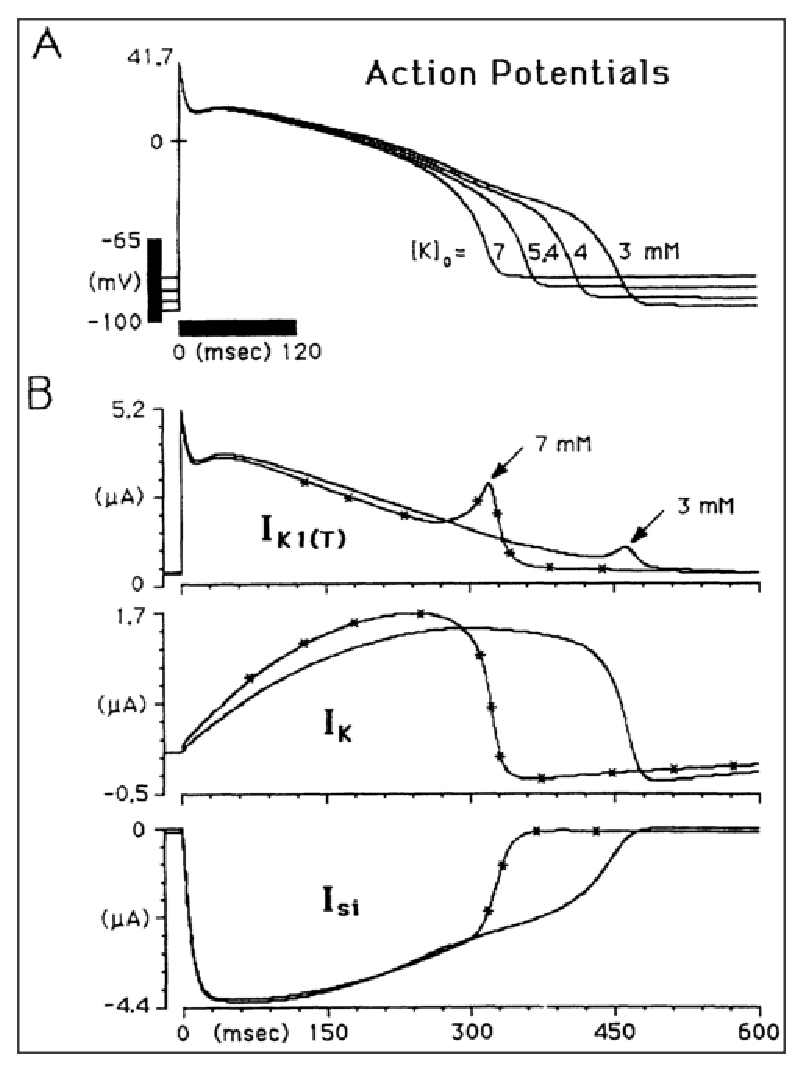
\includegraphics[height=5cm,
    angle=0]{./images/LR1_role_Ko.eps}}
\caption{The role of $[\K]_o$}
\label{fig:LR1_role_Ko}
\end{figure}

The major effects of $[\K]_o$ are on APD and $V_\rest$, not on plateau
potential. $I_{K1(T)}$ depends strongly on $[\K]_o$. With the physiological
value, the following characteristics were observed:
\begin{itemize}
\item resting potential is -84mV

\item threshold for AP is -60mV

\item the overshoot potential is 41.7mV

\item membrane rate of depolarization ($\dot{V}_\max=400$V/sec), which
  is more than 3 times of B-R model (115V/sec), reflects higher
  sodium channel conductance. Compared to E-J model (300V/sec), the
  larger value is due to the higher value in reversal potential
  $E_{\na,LR1}=54.4$mV vs. $E_{\na,EJ}=29$mV causes a greater driving
  force. The difference in reversal potential is due to the different
  in intracellular potential in mammalian ventricular cell
  ([Na]$_i$=18mM) vs. chicken embryo ([Na]$_i$=40mM) used by E-J
  model.

\item maximum plateau potential is 17.7mV

\item AP duration (APD) at 90\% of repolarization $\APD_{90}=336$msec.
\end{itemize}

\begin{figure}[hbt]
  \centerline{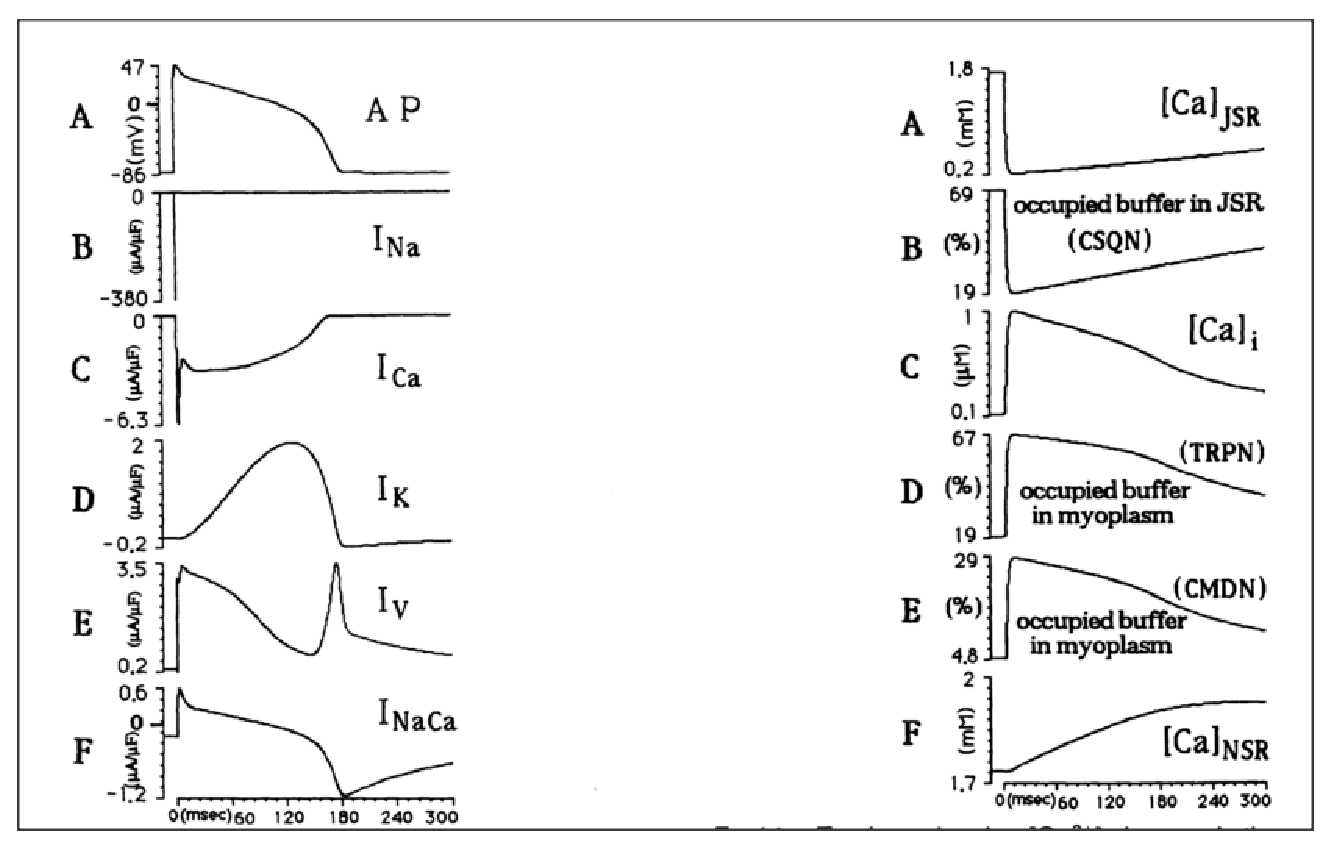
\includegraphics[height=5cm,
    angle=0]{./images/LR1_transient.eps}}
\caption{LR-1 : (A) major ionic currents, (B) concentration transients}
\label{fig:LR1_transient}
\end{figure}

\subsubsection{Simulated Phenomenona}

Also, it can reproduce phenomena that Difrancesco-Noble model could not
simulated, e.g.
\begin{enumerate}
\item supernormal excitability, i.e. the presence of an interval
  during which excitability is longer than the adjacent (previous and
  following), Fig.~\ref{fig:supernormal_excitability}, or aka
  beat-to-beat alternans of APD. 

\begin{figure}[hbt]
  \centerline{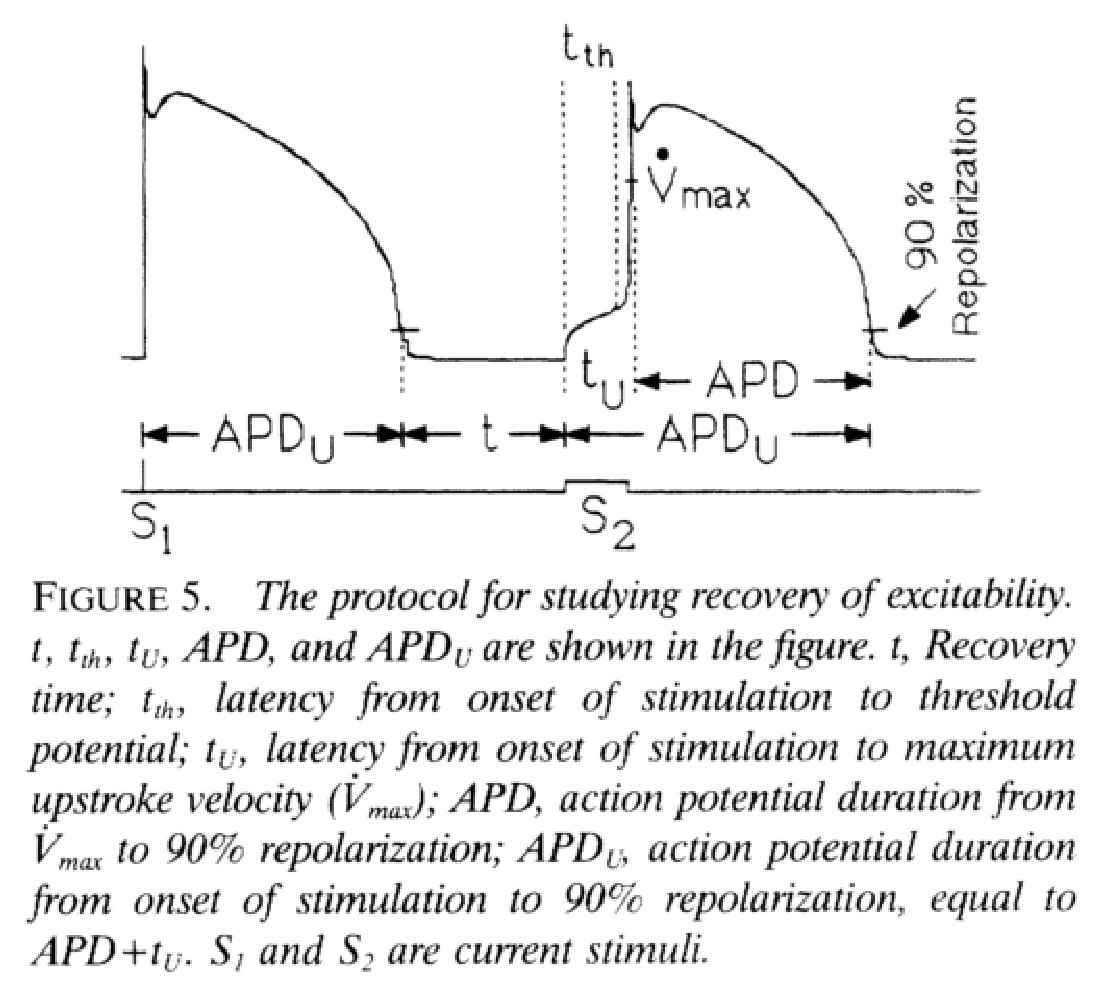
\includegraphics[height=5cm,
    angle=0]{./images/supernormal_excitability.eps}}
\caption{}
\label{fig:supernormal_excitability}
\end{figure}

\item Wenckebach periodicity: which can occur in atrioventricular node or in
  cardiac tissue (when there is a region of depressed conductance
  separating two region of normal excitability) or found recently in a single
  cardiac cell under a periodic stimulation of long stimulation (20ms),
  indicating that the phenomenon is an intrinsic property of the cell membrane
  under various initial  conditions (Sect.\ref{sec:wenck-peri}).

\item aperiodic response of the cell to periodic stimulation under
  different values of $[\K]_o$, that are extremely sensitive to
  initial conditions.
\end{enumerate}

In summary:
\begin{itemize}
\item The inward calcium current (negative) affect the shape of the
  AP.

\item The outward $I_K$ (positive) is set to doubled, then half of its
  default value.

\item Try to find out during what phase of the AP, $I_{K1}$ is
  on. What if we decrease $g_{K1}$ (e.g. 20\% of its normal
  value). What happen if we set $g_{K1}=0$ and run the simulation for
  a long time (3000ms).

\item Try to understand the dynamics of the four ionic currents during
  AP, by plotting and examining the time course of their gating
  variables.

\end{itemize}

The model cannot
\begin{itemize}
\item simulate the effect of elevated extracellular $\ce{K+}$
  concentration, which is an important aspect of ischemia. 
\end{itemize}

\section{Nordin (1993) - guinea pig}

\citep{nordin1993cmm}


\section{Luo-Rudy Phase II (1994) - guinea pig}
\label{sec:luo-rudy-phase-2}


In RL-phase I model (Sect.~\ref{sec:luo-rudy-phase-1}), 6 ionic
currents was examined ($I_{Na}$, $I_\si$, $I_{K}$, $I_{K1}$,
$I_{Kp}$, and $I_b$), with all ion concentrations, except cytosolic
$[\ca]_i$, were assumed to be fixed.  Intracellular $\Ca$
transient cannot be correctly simulated and thus has not been simulated (not
shown in the paper) in LR-1 for many reasons: (1) kinetics of $I_\ca$ was not
correct, (2)  pumps and exchangers was not added, (3) other dynamically
processes  was not incorporated (e.g. $\ca$ reuptake). 

\citep{luo1994dmc_a} completed the model by adding ionic pumps and exchangers to
the model; adjusted the parameters using new data. The model is known as
LR-phase 2 model, Fig.~\ref{fig:LR_phase2}.  
\begin{itemize}
\item In LR-2, $I_\si$ becomes $I_{\ca,t}$ (t=total) whose
  channels permeate up to 3 different types of ions, thus giving 3
  different ionic components $I_\ca, I_\CaK, I_\CaNa$
  (i.e. calcium channel permeate $\Ca,\Na$, and $\K$).
\item non-specific $\Ca$-activated current $I_\nsCa$ which permeate both
$\Na$ and $\K$: $I_\nsNa$, $I_\nsK$.
\item Incorporate ionic pumps and exchangers: 2 exchangers ($I_{Na/K}, I_\NCX$)
+ 1 ATP-driven pump $I_\pCa$. 
\item background currents $I_b$ now becomes $I_\bCa, I_\bNa$.

\item Add intracellular processes that dynamically change $[\ca]_i$,
  e.g. $\Ca$ buffering which is essential for correct simulation
  of Ca transient.
  \item $I_{K1(T)}$ changed the notation to $I_v$ as time-independent
  currents conducting not only $\K$, but also $\Na$ and $\Ca$. 
\end{itemize}
The recent updates of the model are \citep{faber2000}
(Sect.\ref{sec:faber-rudy-model}).

REMEMBER: The volume (L) from which the concentrations are defined is cytosolic
volume, e.g. $[\Ca]_i = 0.12\mu$mol/L = 0.12$\mu$mol/(L-cytosol). 

\subsection{Hypothesis analysis}
\label{sec:hypothesis-analysis-4}

Similar to LR-1:
\begin{itemize}
\item specific membrane capacity is $\Csc=1\mu$F/cm$^2$.
\item data is adjusted to $T=37^\circ$C, using
  $Q_{10}=2.96$~\citep{cavalie1985etc}.

  E.g. with $Q_{10}=3$, at $22^\circ$C, $I_\ca=2\mu A/$cm$^2$, then
  at $37^\circ$C, $I_{\ca,new}= I_\ca (Q_{10})^{(37-22)/10} =
  10.39\mu A/$cm$^2$.
  % NOTE: new value = old value $\times Q_{10}^{(T_{new}-T_{old})/10}$. 

\end{itemize}

LR-2 has some changes
\begin{enumerate}
\item $I_\ca$ inactivation depends both $V_m$ and $[\ca]_i$.
\item $I_\ca$ activation is an order of magnitude faster than LR-1
\item For ion concentrations: In LR-phase 1 model,
  $[\Na]_i=18$mM (at $37^\circ$C), the new measured experimental
  data for intracellular sodium concentration show lower values. So,
  in this model, $[\Na]_i=10$mM (or mmol/L). 

  The initial resting intracellular calcium concentration is now set
  to $[\ca]_i=0.12\mu$mol/L (or $0.12\muM$), which
  agrees with experimental data.
\end{enumerate}

\begin{framed}
In myocardium, L-type $\Ca$ channels is the dominant than
  T-type. Thus, all models for cardiac cells assume L-type $\Ca$
  channels only.

In 1980s, the inactivation process of
$\Ca$ is one of the main controversy subject. Recent data shown  that it is both
$V_m$-dependent and $[\ca]_i$  dependent.~\citep{standen1982bsm} was the first
to formulate  $\Ca$-dependent inactivation for calcium channels
  (Sect.~\ref{sec:standen_1982model}). 
\end{framed}

\begin{figure}[hbt]
  \centerline{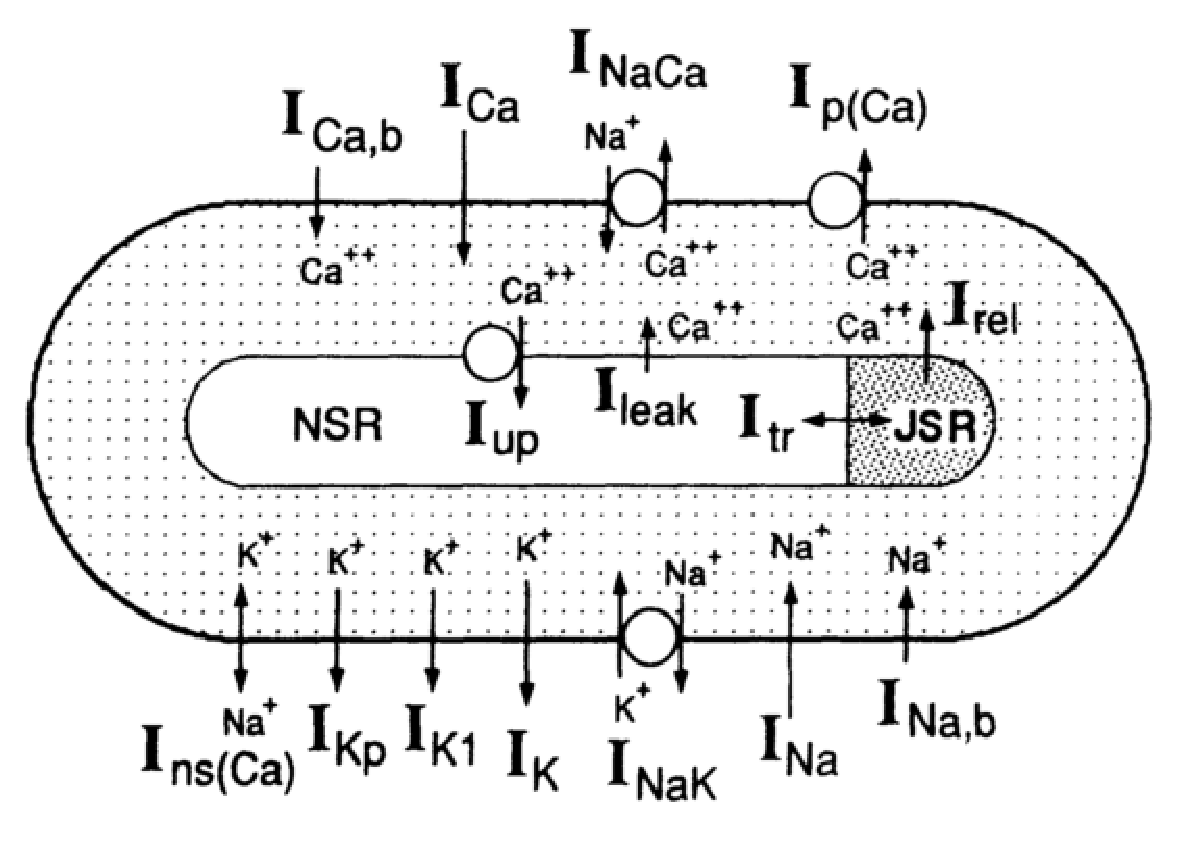
\includegraphics[height=5cm,
    angle=0]{./images/LR_phase2_cell.eps}}
  \caption{Schematic diagram of the cell model. Intracellular
    compartment is the SR (divided into 2 subcompartments: NSR and
    JSR). Dotted areas (in the myoplasm and JSR) indicate the presence
    of $\Ca$ buffer}
  \label{fig:LR_phase2}
\end{figure}

As $\Ca$ cycling is completed before the mechanical relaxation is accomplished
\citep{bers1987,bers1989}, Bers suggested that $\Ca$ pumped back to the SR
is not immediately available for release in the subsequent beat. This delayed reponse of $\Ca$
availability may be attributed to an internal mechanism controlling $\Ca$
release from SR or a relatively slow transport process. To account for the later
hypothesis, SR is often modeled with 2 components: NSR and JSR, where $\Ca$	is
uptake to NSR and then refill to JSR. 

\subsubsection{Buffers}
\label{sec:buffers-3}

Even though the sarcolemmal (SL) can play a role as buffers for $\Ca$, with
very large buffer capacity ($>1$mM), yet it may not play important role to ECC.
Thus, in the model, sarcolemmal buffers were neglected. 
Then, the two main buffers in the myoplasm are
{\bf calmodulin}\footnote{$\Ca$-binding protein in the SR} and
{\bf
  troponin C} (TnC, to initiate contracting force-generating mechanism)
  \footnote{$\Ca$-binding protein in the myofilament}.

Buffering in the JSR is calsequestrin (CSQN). In rat
ventricular myocyte, 68.5\% of CSQN binds to $\Ca$ (resting, no $\Ca$
overload).  Buffers concentration were collected
from~\citep{wier1986}. The kinetics of buffering is
from~\citep{robertson1981}. With the assumption of fast buffering, the
equations for buffering are given in eq.~\eqref{eq:1261}
\begin{equation}
  \label{eq:1261}
  \begin{split}
    [\ca.\TRPN] = [\TRPN]_T\frac{[\Ca]_i}{K_{m,\TRPN}+[\Ca]_i} \\
    [\ca.\CMDN] = [\CMDN]_T \frac{[\Ca]_i}{K_{m,\CMDN}+[\Ca]_i} \\
    [\ca.\CSQN] = [{\CSQN}]_T\frac{[\Ca]_\jsr}{K_{m,\CSQN}+[\Ca]_\jsr} \\
  \end{split}
\end{equation}
with $[\TRPN]_T = 70\muM$, $[\CMDN]_T=50\muM$, $K_{m,\TRPN}=0.5\muM$,
$K_{m,\CMDN}=2.38\muM$; $K_{m,\CSQN}=0.8$mM, $[\CSQN]_T = 10$mM. 


\subsubsection{Ion concentrations}
%\label{sec:ionic-concentrations-1}

All ionic was assumed fixed except myoplasm calcium.  All processes
that affect $[\ca]_i$ are: $I_{\ca,t}, I_\Cab$, $I_\NCX$, a
non-specific $\ce{Ca^2}$-activated current $I_\nsCa$; a Ca pump in
the SR $I_\pCa$, buffering of $\Ca$ ions in the myoplasm and
in the SR, uptake of calcium by the NSR\footnote{network SR} $J_{up}$,
leakage of $\Ca$ from NSR $J_\leak$, and release of $\Ca$
ions from the JSR $J_\rel$.

\begin{framed}
  REMEMBER: The rate of changes of an ionic concentration [B] across the
  membrane is given by
  \begin{equation}
    \label{eq:1253}
    d[B]/dt = -\Csc\frac{(I_B.A_{cap})}{V_C.z_B.F}=-\frac{(I_B'.A_{cap})}{V_C.z_B.F}
  \end{equation}
  with $I_B$ and $I'_B$ are both the sum of ionic currents carrying
  ion B away, except they use different units ($I_B$ use
  ($\muA/\muF$), and $I'_B$ use ($\muA$/cm$^2$)). The choice
  depending upon how we write the equation
  \begin{equation}
    \label{eq:1254}
    \frac{dV_m}{dt} = \sum I_B
  \end{equation}
  or
  \begin{equation}
    \label{eq:1255}
    \Csc \frac{dV_m}{dt} = \sum I'_B
  \end{equation}
  $A_{cap}$ is the total membrane area that functions are capacitance,
  i.e. capacitive membrane area [cm$^2$], $V_C$ is the volume of the
  compartment where [B] is updated, $z_B$ is valence and $F$ is
  Faraday constant.

  As the ionic current is computed based on 1$\muF$ of cell membrane
  capacitance, i.e. unit ($\muA$/$\muF$), we need to multiply to the
  membrane area per 1$\muF$.  In cell, 1$\muF$ correspond to 1cm$^2$
  of cell membrane, i.e. $\Csc=1\mu$F/cm$^2$.  The unit Ampere is
  [C/sec].

  If we use the unit of $I_B$ as ($\muA/\muF$), then $I'_B$ is
  ($\muA$/cm$^2$), so the result of $I'_BA_{cap}$ or $\Csc I_BA_{cap}$ is
  ($\muA$). Next, if each atom carry $z_B$ charges, to convert to the
  amount of moles change, we need divided by $z_BF$ which gives us
  (\verb!mol/sec!). Finally, to convert to concentration change, we
  need to divide by the volume.

  Typically, we assume that capacitance is every where in the
  membrane. Thus, quantitatively, $A_{cap}$ have the same value with the
  whole-cell membrane area $A_m$.
\end{framed}

% \subsubsection{Ionic currents}
% \label{sec:ionic-currents-2}

\subsubsection{$\Na$ current}

B-L formula for fast inward Na current $I_\Na$ was used, with a
minor change in the maximum conductance $\overline{g_{Na}}$ and the
reversal potential $E_{Na}$, eq.~\eqref{eq:940}.

\subsubsection{$\Ca$ current}

With slow-inward calcium current $I_{\ca,t}$, there are some major
changes. To account for both $V_m$ and \ce{[\ca]_i} dependent
inactivation,
\textcolor{blue}{it is assumed that the inactivation can be expressed
  by two separate inactivation gating variables} $f$ and $f_\ca $,
eq.~\eqref{eq:759}. In addition, the $\Ca$ channel permeate not
only to $\Ca$, but also to $\ce{Na+}$ and $\ce{K+}$ though with a
much lower permeability. Thus, the total current via Calcium channel
is
  \begin{equation}
    \label{eq:761}
    I_{\ca,t} = I_\ca +I_\CaK+I_\CaNa
  \end{equation}
  To measure the kinetics for $f$, $\Ca$ was replaced by other
  ions that are not subject of $\Ca$-dependent inactivation,
  e.g. $\ce{Ba^2+}, \ce{Sr^2+}, \ce{K+}, \ce{Na+}$, which give different
  controversial results. There were different proposed formula, yet in LR-phase
  2 model, the formula from Rasmusson {\it et al.} was chosen, eq.~\eqref{eq:762}.
  
\begin{itemize}
\item $f_\infty$ has either partially U-shaped or monotonically
  decreasing
\item $\tau_f$ has bell-shaped or U-shaped. 
\end{itemize}

\begin{framed}
  \begin{enumerate}
  \item use conventional $f_\infty$, Kass \& Sanguinetti $\tau_f$
    \begin{align}
      \label{eq:941}
      f_\infty = \frac{1}{1+\exp(\frac{V_m+30}{8})} \\
      \tau_f = 16.88 + 462.46 \times \frac{\exp(0.092\times(V_m+21.68)}{1.0+\exp(0.246(V_m+21.68))} 
    \end{align}

  \item Hadley and Hume $f_\infty$, Kass \& Sanguinetti $\tau_f$:

    \begin{align}
      \label{eq:942}    
      f_\infty = \frac{0.59}{1+\exp(0.59(V_m+26.12))}+0.41
    \end{align}
  \item Rasmusson {\it et al.} (Sect.~\ref{sec:rasmusson-et-al})
    \begin{align}
      \label{eq:943}
      f_\infty = \frac{1}{1+\exp(\frac{V_m+35.06}{8.6})} + \frac{0.6}{1+\exp(\frac{50-V_m}{20})} \\
      \tau_f = \frac{1}{ 0.0197\exp\left(-(0.0337(V_m+10))^2 \right) + 0.12}
    \end{align}
  \item Difrancesco-Noble model (Sect.~\ref{sec:difr-noble-purk}):
    \begin{align}
      \label{eq:944}
      ...
    \end{align}
  \end{enumerate}
\end{framed}

For $f_\ca$: The $\Ca$-inactivation was first formulated by Standen-Stanfield
which assumed a sub-sarcolemmal space with high ionic calcium concentration from
this space (Sect.~\ref{sec:standen_1982model}). However, LR-phase 2 didn't
consider this compartment (with the claim that not enough data to support the
fact that there is high concentration of calcium near the sarcolemma), i.e.
calcium influx flow directly to myoplasm. Also, \textcolor{red}{the process of
calcium-binding inactivation was assumed
  a fast, with two calcium ions binding to the channel}.
So, Michaelis-Menten-type equation was utilized, eq.~\eqref{eq:385}.
\textcolor{red}{The assumption is wrong, and we'll learn that local evelation is
important}.

\subsubsection{$\K$ current}

$\ce{K+}$ currents:
\begin{itemize}
\item Recent single cell experimental data show that the time-dependent K
  current $I_{K}$ shown a non-linear dependence on the activating gating
  variable, i.e. $X^2$ rather than $X$. With new $I_{\ca,t} $ formula, this
  new formulation of $I_{K}$ also repolarize the membrane potential from
  plateau potential to the resting value even at low $[\ce{K}]_o$,
  eq.~\eqref{eq:760}.

\item There is no major change in the time-independent K current
  $I_{K1}$, except the maximum conductance of the time-independent K
  current was adjusted to the correct value, due to the adding of the new
  $I_{\ca,t} $ formula.

\item The plateau range K current $I_{Kp}$ is the same as that in
  LR-phase 1 model.
\end{itemize}

\subsubsection{Ionic pumps + exchangers}

In this model, the three ionic currents from the electrogenic
pumps/exchangers $I_{Na/K}$, $I_\NCX$ and $I_\pCa$ are
incorporated.
\begin{itemize}
\item The formula
  for Na/Ca exchanger used in DN model (Sect.~\ref{sec:difr-noble-purk})
  was wrong in many ways, as it was not incorporated $[\Na]_o$
  dependency, $[\ca]_o$ dependency, a saturation of $I_\NCX$ at
  very negative potential, eq.~\eqref{eq:770}.

\item Due to the extremely negative reversal potential
  $E_{Na/K}<-200$mV; it is
  \textcolor{red}{assumed that the backward operation of the Na/K
    exchanger doesn't exist}. In forward direction, the pump extrudes
    $3\ce{Na+}$ ions out in exchange for $2\ce{K+}$ ions in. In the formula
    proposed by DN model or Rasmusson {\it et al.}
    (Sect.~\ref{sec:difr-noble-purk}), the $V_m$-dependent has not
    been considered. This was updated in this model,
    eq.~\eqref{eq:771}.

\item As suggested by Rasmusson et al., in addition to the Na/Ca
  exchange, the sarcolemmal $\Ca$ pump $I_\pCa$ is for extrusion of $\Ca$ to
  maintain a low $[\ca]_i$ at rest, eq.~\eqref{eq:772} (\textcolor{red}{later
  models call it} $I_\pmca$ (plasma membrane
    $\Ca$-ATPase)).
\end{itemize}

\subsubsection{Non-specific and background currents}

In 1987, a novel $\Ca$-activated non-specific channel was
discovered in guinea-pig ventricular cells~\citep{ehara1987can}. The
channel is equally permeable to $\ce{K+}$ and $\ce{Na+}$, and much less
permeable to $\Ca$. Thus, the current $I_\nsCa$ was assumed to
be the sum of $I_{ns,Na}$ and $I_{ns,K}$. The formula is derived from
constant field theory with a $\Ca$-activated term using Hill
coefficient $\eta= 3$, eq.~\eqref{eq:765}.

\begin{framed}
  $I_\nsCa$ is suspected to conduct the arrhythmogenic transient
  inward current $I_{TI}$ under $\Ca$-overloaded condition. 
\end{framed}

The background inward $\Ca$ current $I_\bCa$ is formulated as a linear
leak current so that it balances with the loss of calcium via $I_\NCX$ and
$I_\pCa$ at rest to maintain a resting level $[\ca]_{i,rest}=0.12\mu$mol/L,
eq.~\eqref{eq:773}.  LR-phase 1 model doesn't have this current.

In addition to $I_\Cab$, there is also a Na background outward current
$I_\bNa$ which is formulated as a linear leakage current. Its
contribution is to balance with the inwarding $\Na$ via $I_{Na/K}$ and $I_\NCX$
to maintain a steady level $[\Na]_i$ at resting, eq.~\eqref{eq:775}. 

In LR-phase 1 model, the time-independent currents $I_{K1(T)}$ are
hypothesized to be $\ce{K+}$ currents only. In LR-2 model, we have more
components, and the symbol now have to be changed to $I_v$
\begin{equation}
  \label{eq:776}
  I_v = I_{K1}+I_{Kp}+ I_\pCa + I_\bNa + I_\Cab + I_{Na/K}
\end{equation}

\subsubsection{Fluxes}
\label{sec:fluxes-2}

At this point, CICR is widely accepted as a local phenomena in which
$\Ca$ sparks are elementary events~\citep{cheng1993cse}.  The
major internal calcium storage is ER/SR (known as network SR) which is model
with 2 compartments: NSR and junctional SR (JSR), Fig.~\ref{fig:LR_phase2}. 

Finally, to model $\Ca$ signalling pathway inside of the cell
that mimics the CICR process, the calcium subsystem is modelled with 4
fluxes: $J_{up}$ (uptake to NSR), $J_\leak$ (leak from NSR to
cytosol), $J_{tr}$ (transport between NSR and JSR), $J_\rel$ (release
from JSR to cytosol).
\begin{itemize}
\item The translocation of $\Ca$ from the NSR to the
  JSR\footnote{junctional SR} is $J_{tr}$ and was modeled as a
  mono-exponential function, eq.~(\ref{eq:974}).

\item With a small volume fraction of JSR (0.48\%) and slow rate of
  $\ca$ uptake, the $\ca$ uptake from the myoplasm by the JSR was
  considered neglected and $\ca$ enters the JSR was modeled with a
  single pathway, i.e. from the NSR via $J_{tr}$. The $\ca$ uptake to
  the NSR $J_{up}$ was modeled with a SERCA pump using
  Michaelis-Menten type equation,
  eq.~\eqref{eq:1260}~\citep{haynes1987}.

\item $J_\leak$ was modeled with the leak rate was chosen to retain
  the maximum $[\ca]_\nsr=15$ mM at resting, i.e. , eq.~(\ref{eq:975})
\end{itemize}


\subsection{Mathematical model}
\label{sec:mathematical-model-11}

The derivative of the membrane potential is given
\begin{equation}
  \label{eq:1263}
  \Csc\frac{dV_m}{dt} = -(\sum I_{ion} + I_{app})
\end{equation}
with $\Csc=1\mu$F/cm$^2$ closed to experimental value in literature.

\subsubsection{Ionic currents}
\label{sec:ionic-currents-6}

\begin{enumerate}
\item fast inward Na current $I_{Na}$, the same as eq.~\eqref{eq:724},
  with some changes in values
  \begin{equation}
    \label{eq:940}
    I_{Na}= \overline{g_{Na}} * m^3 * h * j * (V_m - E_{Na})
  \end{equation}
  \begin{itemize}
  \item $E_{Na} = 70$mV 
  \item $\overline{g_{Na}}=16$mS/cm$^2$ - still in the physiological
    range (to compensate for the increase in $E_{Na}$ and keep the
    peak Na current the same (380$\muA$/$\muF$))
  \end{itemize}

\item the inward Calcium current via L-type channel (DHPR) show a
  permeability to multiple ions $\Ca, \ce{Na+}$ and $\ce{K+}$
  with the ratio 2800:3.5:1.

  \begin{equation}
       \label{eq:759}
       \begin{split}
         I_\ca  = \overline{I_\ca } d.f.f_\ca  \\
      I_\CaK = \overline{I_\CaK} d.f.f_\ca  \\
      I_\CaNa = \overline{I_\CaNa}.d.f.f_\ca 
    \end{split}
  \end{equation}
NOTE: DN model use $f_2$ instead of $f_\ca $ notation. 

The formula of $\overline{I_\ca }, \overline{I_\CaK},
\overline{I_\CaNa}$ are estimated using constant field theory,
eq.~\eqref{eq:621}, with
\begin{itemize}
\item $P_\ca  = 5.4\times 10^{-4}$cm/s, $\gamma_{Ca,i}=1,
  \gamma_{Ca,o}=0.341$
\item $P_{Na} = 6.75\times 10^{-7}$cm/s, $\gamma_{Na,i}= \gamma_{Na,o}=0.75$
\item $P_{K} = 1.93\times 10^{-7}$cm/s, $\gamma_{K,i}= \gamma_{K,o}=0.75$
\end{itemize}
The two $V_m$-dependent gating variables $d,f$ have
\begin{equation}
  \label{eq:762}
  \begin{split}
    \alpha_d = \frac{d_\infty}{\tau_d} \; \; ;
    \beta_d = \frac{1-d_\infty}{\tau_d} \\
    \alpha_f =  \frac{f_\infty}{\tau_f} \;\; ;
    \beta_f = \frac{1-f_\infty}{\tau_f} \\
     f_\infty = \frac{1}{1+\exp[\frac{V_m+35.06}{8.6}]} +
     \frac{0.6}{1+\exp[\frac{50-V_m}{20}]} \\
     \tau_f = \frac{1}{0.0197\exp\left[-0.0337 (V_m+10)^2
       \right]+0.02} \\
     d_\infty =\frac{1}{1+\exp[-\frac{V_m+10}{6.24}]} \\
     \tau_d = d_\infty
     \frac{1-\exp[-\frac{V_m+10}{6.24}]}{0.035(V_m+10)} 
  \end{split}
\end{equation}

The $\Ca$-inactivating gating variable $f_\ca $ is
\begin{equation}
  \label{eq:385}
  f_\ca  = \frac{(K_{m,Ca})^2}{(K_{m,Ca})^2 +
    \left([\Ca]_i\right)^2} = \frac{1}{1 + \left(\frac{[\Ca]_i}{K_{m,Ca}}\right)^2}
\end{equation}
with $K_{m,Ca}=0.6\mu$mol/L is the calcium concentration that produce
half-maximal calcium inactivation.

\item the time-dependent K current $I_K$
\begin{equation}
  \label{eq:760}
  I_K = \overline{g_{K}} \times X^2 \times X_i\times (V_m-E_K)
\end{equation}
with
\begin{equation}
  \label{eq:766}
  X_i = \frac{1}{1+\exp[\frac{V_m-56.26}{32.1}]}
\end{equation}
and
\begin{equation}
  \label{eq:767}
  \begin{split}
      \alpha_x = 7.19\times 10^{-5}
      \frac{V_m+30}{1-\exp[-0.148(V_m+30)]} \\
      \beta_x = 1.31\times 10^{-4} \frac{V_m+30}{-1+\exp[0.0687(V_m+30)]}
  \end{split}
\end{equation}

\item time-independent K current $I_{K1}$: there is only minor change
  $\overline{g_{K1}}=0.75$mS/$\muF$. 

\item the plateau range K current $I_{Kp}$ (the same as LR-phase 1)

\item the $\ce{Na+}/\ce{Ca^2}$ exchanger $I_\NCX$, with stoichiometry 3Na:1Ca.
\begin{equation}
  \label{eq:770}
  \begin{split}
      I_\NCX = k_\NCX \frac{1}{K^3_{m,Na}+[\Na]_o^3}
      \frac{1}{K_{m,Ca}+[\ca]_o}\frac{1}{1+k_{sat}\exp[(\eta-1).\frac{V_m}{RT/F}]}
      \\
      \left(\exp[\eta\frac{V_m}{RT/F}] [\Na]_i^3 [\ca]_o -
        \exp[(\eta-1)\frac{V_m}{RT/F}] [\Na]_o^3 [\ca]_i\right)
  \end{split}
\end{equation}
with scaling factor $k_\NCX=2000\mu$A/$\muF$; Na half-saturation
constant $K_{m,Na}=87.5$ mmol/L and Ca half-saturation constant
$K_{m,Ca}=1.38$ mmol/L; and $k_{sat}=0.1$ is the saturation factor
that ensure saturation at very negative potential (later models use
$k^{sat}_\ncx$); $\eta=0.35$ the position of the energy barrier that
control $V_m$-dependent (later models use $\eta_\ncx$).

\item the $\ce{Na+}/\ce{K+}$ exchanger $I_{Na/K}$ with 3Na:2K.
  \begin{equation}
    \label{eq:771}
    I_{Na/K} = \overline{I_{Na/K}} f_{Na/K}
    \frac{1}{1+\left(\frac{K_{m,Na_i}}{[\Na]_i}\right)^{1.5}} \frac{[\ce{K}]_o}{[\ce{K}]_o+K_{m,K_o}}
  \end{equation}
  with $\overline{I_{Na/K}}=1.5\mu$A/$\muF$; $K_{m,Na_i}=10$mmol/L;
  $K_{m,K_o}=1.5$ mmol/L.  $f_{Na/K}$ is the $V_m$-dependent gating
  variable.
  \begin{equation}
    \label{eq:764}
    f_{Na/K} = \frac{1}{1+0.1245\exp[-0.1\frac{V_m}{RT/F}]+0.0365 \sigma \exp(-\frac{V_m}{RT/F})}
  \end{equation}
with $\sigma = \frac{1}{7}[\exp(\frac{[\Na]_o}{67.3}) -1 ]$.

\item the $\Ca$-activated non-specific channel $I_\nsCa$
\begin{equation}
  \label{eq:765}
  \begin{split}
      I_\nsCa = I_{ns,K} + I_{ns,Na} \\
      I_{ns,K} = \overline{I_{ns,K}}
      \frac{1}{1+\left(\frac{K_{m,ns(Ca)}}{[\ca]_i}\right)^3} \\
      I_{ns,Na} = \overline{I_{ns,Na}}
        \frac{1}{1+\left(\frac{K_{m,ns(Ca)}}{[\ca]_i}\right)^3} \\
  \end{split}
\end{equation}
with $K_{m,ns(Ca)} = 1.2\mu$mol/L;
$\overline{I_{ns,K}},\overline{I_{ns,Na}}$ was computed based on
constant field theory as given in eq.~\eqref{eq:621} (using the same
$\gamma$ values as in the inward Calcium current $I_\ca $, yet now
with $P_\nsCa = 1.75\times 10^{-7}$ cm/s (based on
$\overline{g_\nsCa}=0.072$ mS/$\muF$).  The reversal potential was
computed using GHK equation
\begin{equation}
  \label{eq:769}
  E_\nsCa = \frac{RT}{F} \ln\frac{[\ce{K}]_o+[\Na]_o}{[\ce{K}]_i+[\Na]_i}
\end{equation}

\item the sarcolemma $\Ca$ pump $I_\pCa$
  (Sect.~\ref{sec:haynes-madveno-1987}).
\begin{equation}
  \label{eq:772}
I_\pCa = \overline{I_\pCa} \frac{[\ca]_i}{K_{m,p(Ca)}+ [\ca]_i}  
\end{equation}
with $K_{m,p(Ca)}=0.5\mu$mol/L, and $\overline{I_\pCa} =
1.15\mu$A/$\muF$. 

Maximum $[\ca]_\nsr$ is 15mM, with the Hill coefficient is 1, and
half-saturation $K_{m,up}=0.92\mu M$. A maximum reuptake
$\overline{J}_{up}$ larger than 0.003mM/ms is required to reload into NSR
all release $\ca$ during an AP. So, $\overline{J}_{up}=0.005$ mM/ms was
chosen. 

\item (2) background currents
  \begin{itemize}
  \item $I_\Cab$
    \begin{equation}
      \label{eq:773}
      I_\Cab = \overline{g_\Cab}(V_m-E_\Cab)
    \end{equation}
    with $\overline{g_\Cab} = 0.003016$mS/$\muF$, and
    \begin{equation}
      \label{eq:774}
      E_\Cab = \frac{RT}{2F} \ln \frac{[\ca]_o}{[\ca]_i}
    \end{equation}
  \item $I_\bNa$

    \begin{equation}
      \label{eq:775}
      I_\bNa = \overline{g_\bNa} (V_m-E_\bNa)
    \end{equation}
    with $\overline{g_\bNa} = 0.00141$mS/$\muF$; and $E_\bNa=E_{Na}$. 
  \end{itemize}
\end{enumerate}

\begin{framed}
  \begin{equation}
    \label{eq:1262}
    I_v = I_{K1} + I_{Kp} + I_{p(\ca)} + I_\Nab + I_\Cab + I_\NaK
  \end{equation}
is the total ionic currents via sarcolemma. 
\end{framed}

\subsubsection{Fluxes}
\label{sec:fluxes-8}

\begin{enumerate}
\item the uptake of $\Ca$ by SERCA-pump 
  \begin{equation}
    \label{eq:1260}
    J_{up} = \overline{J_{up}} \frac{[\Ca]_i}{K_{m,up}+[\Ca]_i}
  \end{equation}
  with $\overline{J_{up}} = 0.005$mM/ms, $K_{m,up}=0.92\muM$. 

\item to balance the uptake at resting, $J_\leak$
  \begin{equation}
    \label{eq:975}
    J_\leak = K_\leak [\ca]_\nsr
  \end{equation}
  with $K_\leak = \overline{J}_{up}/\overline{[\ca]_\nsr} = 0.000333$ ms${-1}$,
  and $\overline{[\Ca]_\nsr} = 15$mM.

\item the translocation (refill) current $I_{tr}$ from NSR to JSR
  \begin{equation}
    \label{eq:974}
    J_{tr} = \frac{[\ca]_\nsr-[\ca]_\jsr}{\tau_{tr}} \;\; (mM.s^{-1})
  \end{equation}
  with time constant $\tau_{tr} = 180$ ms (experimental data was
  $\tau_{tr}=182\pm44 (ms)$, $\tau_{tr}=176\pm18 (ms)$)


\item the release of $\Ca$ from JSR due to CICR
  \begin{equation}
    \label{eq:1292}
    J_\rel = G_\rel ([\Ca]_\jsr-[\Ca]_i)  \;\;\text{ mM/sec} 
  \end{equation}
and using a heuristic formula
\begin{itemize}
\item Under normal condition
  \begin{enumerate}
  \item If $\Delta [\Ca]_{i,2} \ge \Delta [\Ca]_{i,th}$ at 2 ms after
    $\dot{V}_\max$, then the rate of release is
    \begin{equation}
      \label{eq:1293}
      G_\rel = \overline{G}_\rel \frac{\Delta [\Ca]_{i,2} - \Delta [\Ca]_{i,th}}{K_{m,\rel}+\Delta [\Ca]_{i,2} - \Delta [\Ca]_{i,th}}.(1-\exp(-t/\tau_{on})).\exp(-t/\tau_{off})
    \end{equation}
    with the threshold $ \Delta [\Ca]_{i,th}=0.18\muM$,
    $K_{m,\rel}=0.8\muM$, $\tau_{on}=\tau_{off}=2$ms, $t=0$ at time of
    CICR, and 
    \begin{itemize}
    \item $\overline{G}_\rel = 18$ ms$^{-1}$ for $V_m$-clamp
    \item $\overline{G}_\rel = 60$ ms$^{-1}$ for $I_\stim$-clamp 
    \end{itemize}
  \item If $\Delta [\Ca]_{i,2} < \Delta [\Ca]_{i,th}$ at 2 ms after
    $\dot{V}_\max$, then $G_\rel=0$
  \end{enumerate}
\item Under $\Ca$ overload condition
  \begin{enumerate}
  \item If buffered $[\CSQN] \ge [\CSQN]_{th}$
    \begin{equation}
      \label{eq:1294}
      G_\rel = \overline{G}_\rel .(1-\exp(-t/\tau_{on})).\exp(-t/\tau_{off})
    \end{equation}
    with $\overline{G}_\rel = 4$ ms$^{-1}$, the threshold $[\CSQN]_{th}=0.7$ or
    higher, and  $\tau_{on}=\tau_{off}=2$ms, $t=0$ at time of
    spontaneous release.
  \item  If buffered $[\CSQN] < [\CSQN]_{th}$, then $G_\rel = 0$
  \end{enumerate}
\end{itemize}
\end{enumerate}

\subsection{Units}
\label{sec:units-2}

All ionic currents are computed for 1$\muF$ of cell membrane
capacitance. As specific membrane capacity is set at $1\mu$F/cm$^2$,
we have that 1$\muF$ implies 1cm$^2$ membrane area. 

The formulation is based on experimental data adjusted to 37$^o$F with
$Q_{10}=2.96$. 

\subsection{Cell geometry}
\label{sec:cell-geometry}


The cell is modeled as a cylinder with $L=100\mu$m in length and
$r=11\mu$m in radius. Then, the cell volume $V_{cell}$ is
\begin{equation}
  \label{eq:758}
  V_{cell} = \pi r^2L = 38\times 10^{-6}\mu L
\end{equation}
and the geometric membrane area is
\begin{equation}
  \label{eq:1258}
   A_\geo = 2\pi r^2 + 2\pi rL = 0.767\times 10^{-4} \text{ cm}^2
\end{equation}

Due to the large degree of membrane folding, the actual surface area
$A_m$ is larger than that calculated from the cylinder surface area
$A_{geo}$. Let's define $R_{CG} = A_m/A_{geo}$.

Assuming the specific membrane capacitance $\Csc=1\mu$F/cm$^2$; the
ratio was $\frac{\Cm}{\Csc}$ was found to be approximately to 2 from
different trials and was set to 2, then
\begin{equation}
  \label{eq:725}
  R_{CG} = \frac{\Cm}{\Csc} = 2
\end{equation}
or
\begin{equation}
  \label{eq:1259}
  A_m = 2 A_\geo = 1.534\times 10^{-4} \text{ cm}^2
\end{equation}
If we assume the capacitance is every where on the membrane, then the
capacitive membrane area $A_{cap}=A_m$.

Inside the cell, there are other components, with volume
\begin{enumerate}
\item mitochondria: $V_\mito = V_\cell .26\% = 9.88 \text{ pL}$.  The
  mitochondria volume fraction $F_{mito}$
  \begin{equation}
    \label{eq:755}
    F_{mito} = 26\%
  \end{equation}

\item SR : $V_\sr = V_\cell . 6\% = 2.28 \pL $. According to the CICR
  process~\citep{fabiato1975cic}, the internal $\Ca$ storage was
  divided into 2 compartments: JSR ($8\%$) and NSR ($92\%$). If we set
  the volume fraction of SR compared to cell volume $F_{SR}$ is
  \begin{equation}
    \label{eq:753}
    F_\sr = \frac{V_{SR}}{V_{cell}} = 6\% 
  \end{equation}
  Thus, we have
  \begin{equation}
    \label{eq:754}
    \begin{split}
      F_\jsr = \frac{V_\jsr}{V_{cell}} = 0.48\%  \\
      F_\nsr = 5.52\%
    \end{split}
  \end{equation}
  Finally
  \begin{itemize}
  \item NSR: $V_\nsr = V_\cell . 5,52\% = 2.098 \pL$
  \item JSR: $V_\jsr = V_\cell . 0.48\% = 0.182 \pL$
  \end{itemize}

\item myoplasm: $V_\myo = V_\cell .68\% = 25.84 \text{ pL}$

  As the result, the remaining volume is occupied by the myoplasm
  \begin{equation}
    \label{eq:756}
    F_\myo = \frac{V_\myo}{V_{cell}} = (1-6\%-5.52\%-26\%) = 67.88\%
  \end{equation}

\item cleft : $V_\text{cleft} = (V_\cell/88\%).12\% = 5.182\pL$. For considering ion accumulation in the extracellular space, a cleft
  space was assumed with volume ratio
  \begin{equation}
    \label{eq:757}
    \frac{F_{cell}}{F_{cleft}} = \frac{88\%}{12\%}
  \end{equation}
\end{enumerate}


\subsection{Numerical analysis}
\label{sec:numerical-analysis-2}

Typically, the change in calcium buffered follow the equation
\begin{equation}
  \label{eq:1295}
  \frac{d[\ca.B]}{dt} = f([\ca],[\B])
\end{equation}
Using steady-state assumption, e.g.  $\frac{d[\ca.\CSQN]}{dt} =0$, the
value of calcium buffering $[\Ca]$ in the JSR and myoplasm are
estimated using Steffensen's iterative
method\footnote{method to find the root of an equation} for the
equations $f([\ca],[\B])=0$ (NOTE:~\citep{zeng1995} proposed an
analytical formula (Sect.~\ref{sec:zeng-et-al})).


\subsection{Analysis}
\label{sec:analysis-11}

As calcium release is induced by calcium in the myoplasm in the model, CICR
occur if $[\Ca]_i > 0.18 \muM$ in the first 2ms of the AP. From the beginning of
the stimulus that generate an AP, a delay from 3-9 ms for the $\Ca$ to increase
quickly as a result of CICR and reaches its peak in an additional of 8-19ms.

The model was used to study~\citep{luo1994dmc_b}
\begin{enumerate}
\item phenomena related to ECC, e.g. postextrasystolic mechanical
  potential
\item $\Ca$ overload condition
\item arrhythmogenic activity of the single cell, e.g. early and
  delayed after-depolarization and triggered activity
\end{enumerate}
The model could also be used to study certain aspect of ischemia, or
the effect and mechanism of channel blockers or other anti-arrhythmic
drugs.

LR-2 is also a deterministic model.  A correct model of the AP is not
only to study the behavior of a single cell, but also to the study of
the propagation of excitation in cardiac tissues. However, the model
cannot correctly simulate important aspects of the AP, and situations
of physiological and clinical importance, e.g. $\Ca$ overload,
the effect of $\Ca$ blockers, abnormal propagation
(e.g. reentrant arrhythmias). \textcolor{red}{$\Ca$ transient in the model has
triangular shape, which is not correct}.


\section{Zeng et al. (1995) - guinea pig}
\label{sec:zeng-et-al}

In guinea pig, the delayed rectifier potassium channels was discovered to be a
composite of two channel types (IKr, IKs). The kinetics of the two currents were
studied by \citep{sanguinetti1990tcc, chinn1993} where the delayed rectifier
tail current can be fit by the sum of two exponential functions having fast
($\sim$ 125ms) and slow ($\sim$ 750ms) decay time constants. So, the fast
component can reach the plateau amplitude within 0.5ms, while the slow component
takes 3-6ms.

Based on that data, ~\citep{zeng1995, zeng1995ead} updated LR-2 model for guinea
pig (Sect.~\ref{sec:luo-rudy-phase-2}) with the time-dependent $I_\k$ is
replaced by 2 distinct currents: $I_\Kr,I_\Ks$, Fig.\ref{fig:Zeng_LR2}. In
addition, the calcium current via T-type channel $I_\CaT$ is added into the
model (though its contribution is not significant). $I_\Kr$ and $I_\Ks$ both
were found in guinea-pig ventricular cells, and also atrial cells. The model was
then used to study EAD and its rate dependence \citep{zeng1995ead}.

To adjust with these changes, a small change in plateau-range K current
$I_{\Kp}$ is the maximum conductance $\overline{g_\Kp}=0.00552$ mS/$\muF$ (based on whole-cell
patch-clamp protocol~\citep{backx1993}) rather than using data from
single channel recording as mentioned in~\citep{luo1991mcap} with
0.0183 mS/$\muF$.


\begin{figure}[hbt]
  \centerline{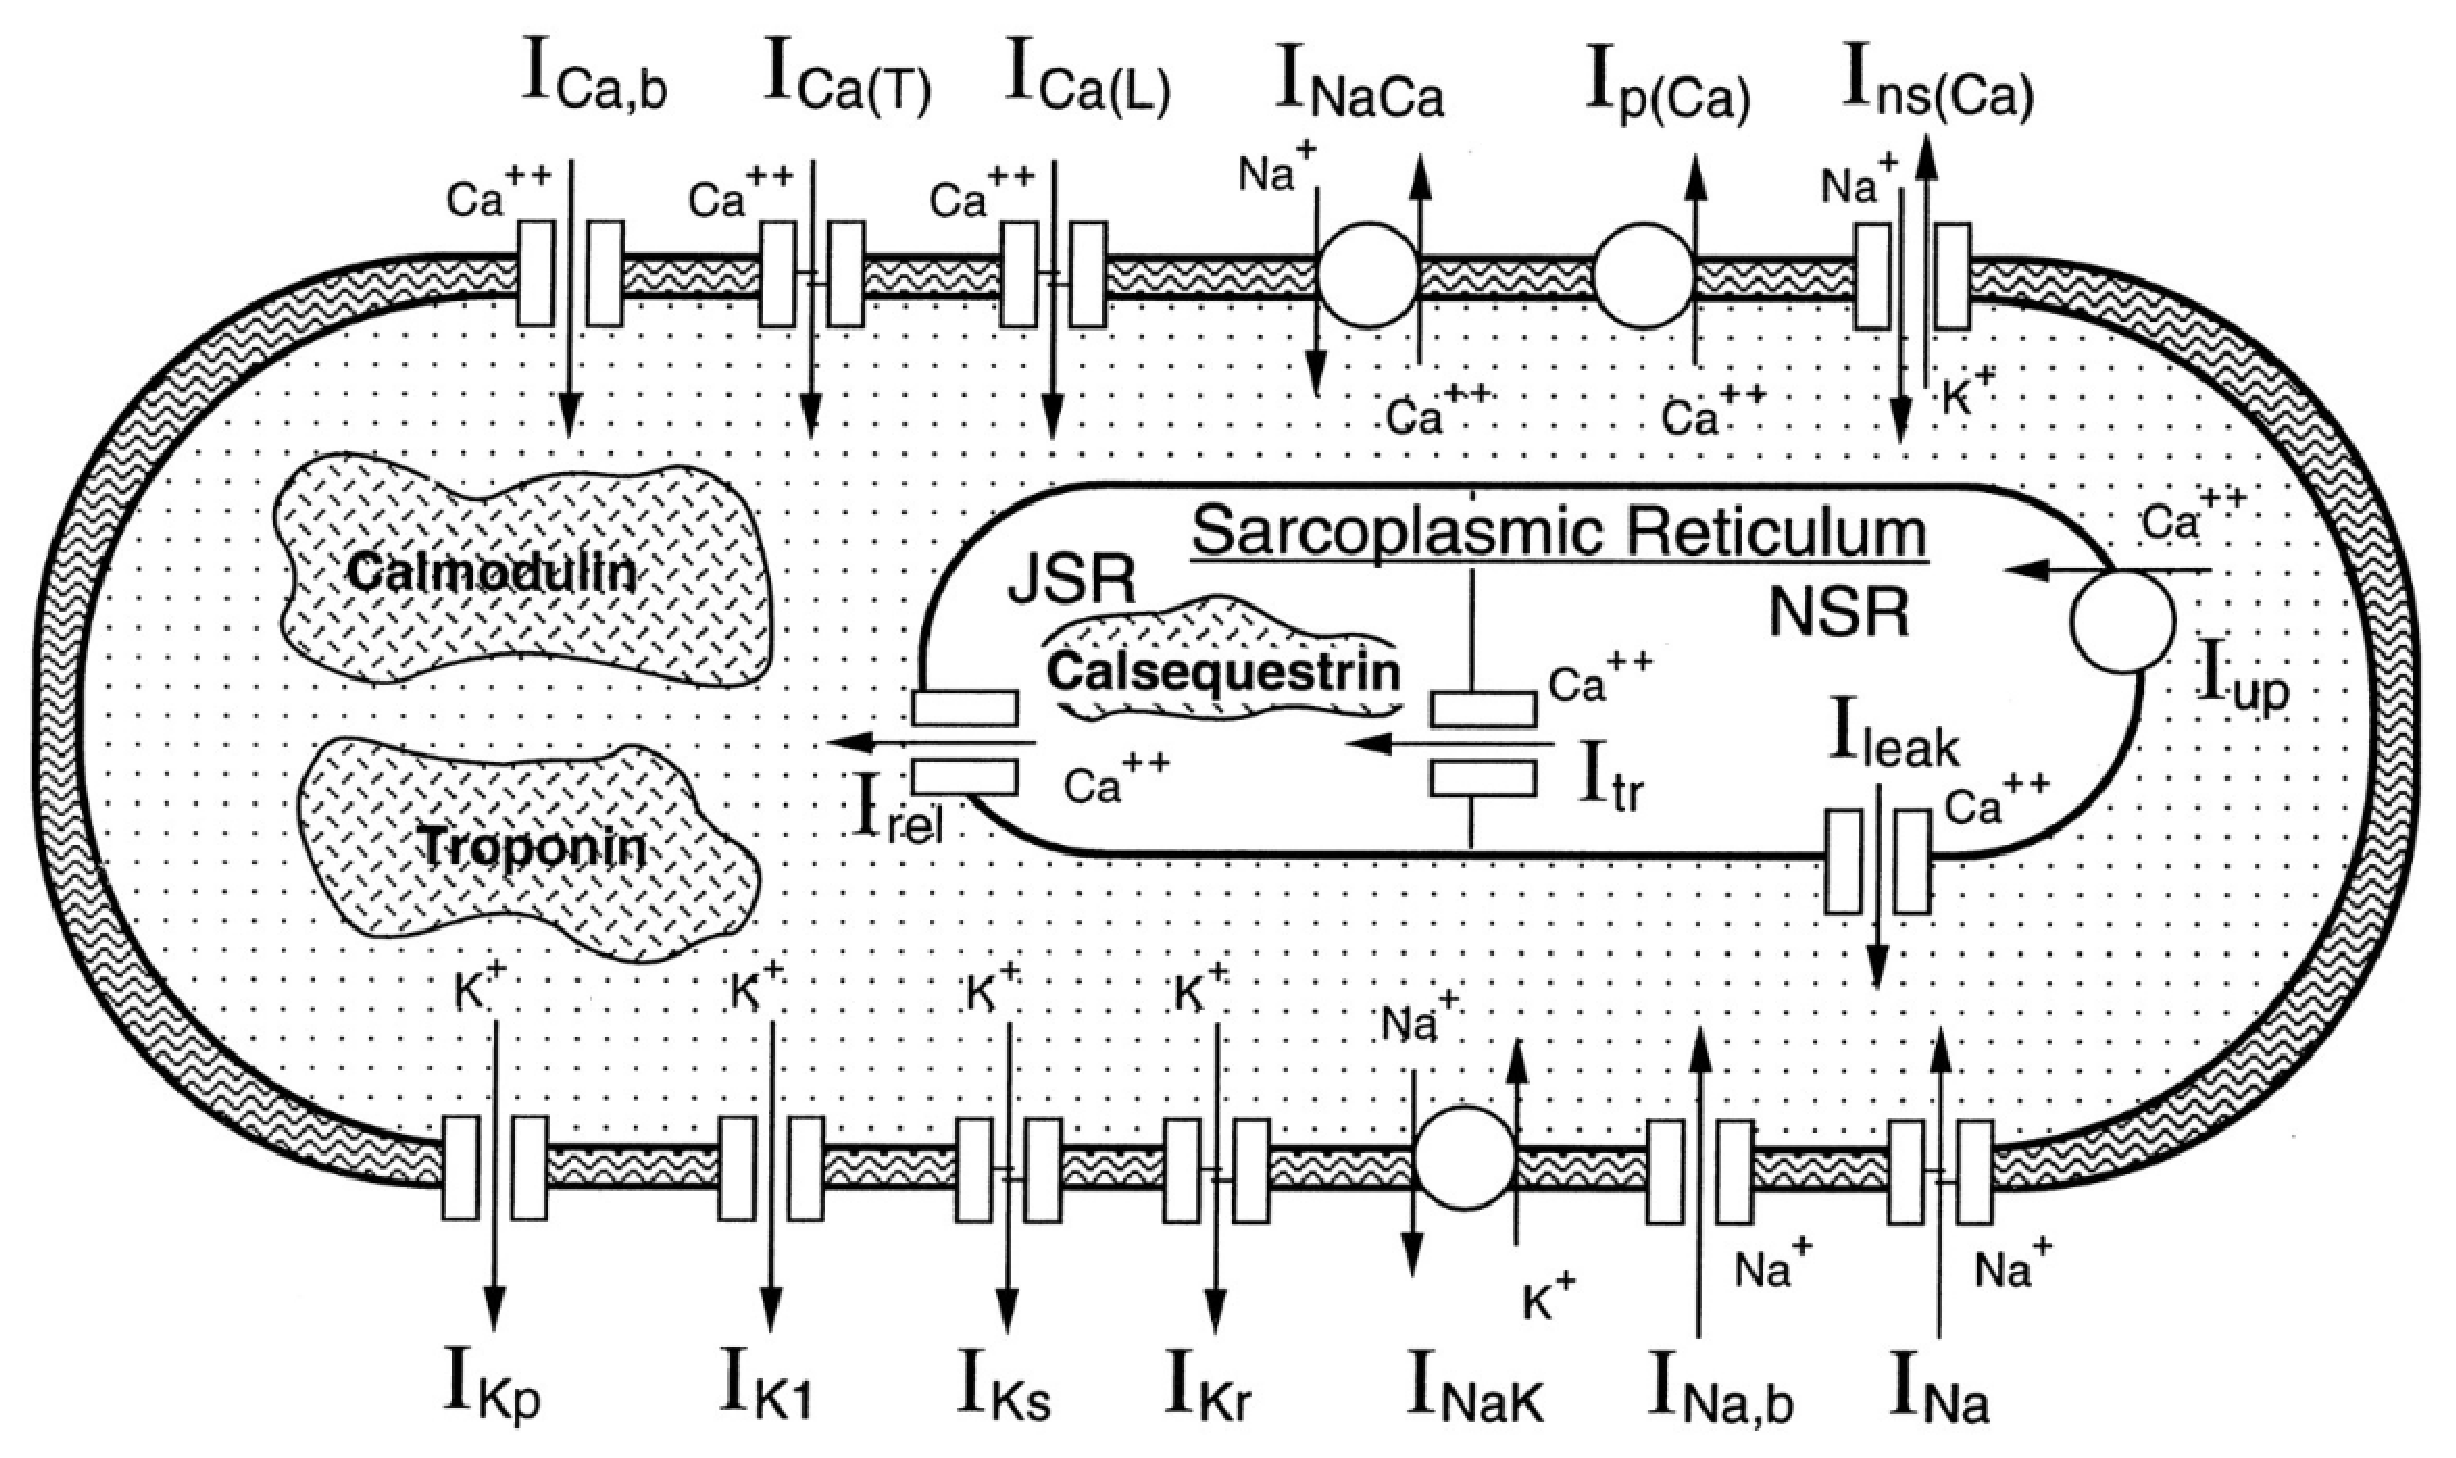
\includegraphics[height=5cm,
    angle=0]{./images/Zeng_LR1.eps}}
\caption{Updated LR-2 model}
\label{fig:Zeng_LR2}
\end{figure}

\subsection{Hypothesis analysis}

\subsubsection{Time-dependent $\K$ current: $I_\Kr, I_\Ks$}
\label{sec:i_k-rightarrow-i_kr}

$I_\Kr$ is purely selective to $\K$ so the reversal potential is modeled using
Nernst equation. $I_\Ks$ is nor purely selective to $\K$, so the reversal
potential is modeled using GHK equation, eq.\ref{eq:1307}.

\begin{framed}
  NOTE:
  \begin{equation}
    \label{eq:1310}
    \frac{dX_\Ks}{dt} = \frac{X_{s,\infty}-X_s}{\tau_{s,\infty}}
  \end{equation}
\end{framed}

The results shown that
\begin{enumerate}
\item $I_\Ks$ is the major outward current during plateau
  repolarization 
\item $I_\Ks$ is sensitive to $[\Ca]_i$.
\end{enumerate}

\subsubsection{T-type $\Ca$ channel}

The T-type calcium current $I_{\ca(T)}$ is modeled in eq.\ref{eq:1304}.
% \begin{equation}
%   \label{eq:1051}
%   I_{\ca(T)} = \overline{G}_{\ca(T)}.b^2.g.(V_m-E_\ca)
% \end{equation}

\subsection{Mathematical model}

\begin{enumerate}
  \item  $I_\Kr$ (or $I_\text{Kr}$) is the prominent inward rectification
  current
\begin{equation}
  \label{eq:1049}
  I_\Kr = \overline{G}_\Kr . f([\K]_o). X_r . R . (V_m - E_\Kr)
\end{equation}
with $\overline{G}_\Kr = 0.02614$, $f([\K]_o)=\sqrt{\frac{[K]_o}{5.4}}$,
$X_r$ is time-dependent inactivation gate, and $R$ is the
time-independent inactivation gating variable
(\textcolor{red}{The inclusion of $R$ introduces the
  inward-rectification property of} $I_\Kr$). As $I_\Kr$ is purely
  selective to $\K$, so $E_\Kr$ is set to reversal potential of $\K$.
  
  
\begin{eqnarray}
  \label{eq:1055}
  E_\Kr = \frac{RT}{z_\k F}.\ln\frac{[\K]_o}{[\K]_i}
\end{eqnarray}
with the valence $z_\k=1$. 
Based on ~\citep{sanguinetti1990tcc}
\begin{eqnarray}
  \label{eq:1058}
  X_{r,\infty} = \frac{1}{1+\exp(-\frac{V_m+21.5}{7.5})} \\
  \tau_{r,\infty} = \left( \frac{0.00138(V_m+14.2)}{1-\exp(-0.123(V_m+14.2))}+\frac{0.00061(V_m+38.9)}{\exp(0.145(V_m+38.9))-1}\right)^{-1}
\end{eqnarray}

\item $I_\Ks$ show no inward rectification. Upon depolarization, it follows
a sigmoidal time course, rather than a single exponential
function. So, using a Hill coefficient of 2 for the gating variable
$X_s$ is better fit
\begin{equation}
  \label{eq:1050}
  I_\Ks = \overline{G}_\Ks.X^2_s . (V_m - E_\Ks)
\end{equation}
As $I_\Ks$ has been found to be sensitive to $\Ca$, $\overline{G}_s$ is
introduced as a function of $[\Ca]_i$
\begin{equation}
  \label{eq:1308}
  \overline{G}_\Ks = 0.057+\frac{0.19}{1+\exp(\frac{-7.2-\log([\Ca]_i)+3}{0.6})}
\end{equation}
and
\begin{equation}
  \label{eq:1309}
  \begin{split}
    X_{s,\infty} = \frac{1}{1+\exp(-\frac{V_m-1.5}{16.7})} \\
    \tau_{s,\infty} = \left( \frac{7.19e-5(V_m+30)}{1-\exp(-0.148(V_m+30))}+\frac{1.31e-4(V_m+30)}{\exp(0.0687(V_m+30))-1}\right)^{-1}
  \end{split}
\end{equation}

Besides, Ks channel is not purely selective to $\K$ like Kr channel,
so the reversal potential is modeled as
\begin{equation}
  \label{eq:1307}
  E_\Ks = \frac{RT}{z_\k F} \ln \frac{[\K]_o +
    P_{\na,\k}[\Na]_o}{[\K]_i + P_{\na,\k} [\Na]_i}
\end{equation}
with $P_{\na,\k}=0.01833$ is permeability ratio between sodium and potassium.

\end{enumerate}

\subsubsection{Finding $[\Ca]_\jsr, [\Ca]_i$}
\label{sec:finding-ca_jsr-ca_i}


Instead of using Steffensen's iterative method
like~\citep{luo1994dmc_a} based on steady-state assumption, they provided
an analytical formula to calculate the concentration of free calcium
in JSR and myoplasm.
\begin{equation}
  \label{eq:1296}
  [\ca]_{\jsr,\new} = \frac{\sqrt{b_1^2 + 4\times c_1} - b_1}{2}
\end{equation}
with
\begin{equation}
  \label{eq:1297}
  \begin{split}
    b_1 &= \overline{[\ca\cdot\CSQN]}-[\ca\cdot\CSQN]_\old - \Delta
    [\Ca]_\jsr - [\Ca]_{\jsr,\old}+K_{m,\CSQN} \\
    c_1 &= K_{m,\CSQN}([\ca\cdot\CSQN]_\old+\Delta [\Ca]_\jsr + [\Ca]_{\jsr,\old})
  \end{split}
\end{equation}
with $\overline{[\ca\cdot\CSQN]}$ is the maximum concentration of $\Ca$
 buffered by CSQN in JSR. 


 \begin{equation}
   \label{eq:1298}
   [\Ca]_{i,\new} = \frac{2}{3}\sqrt{b^2-3.c}\times \cos\left( \frac{\arcos[\frac{9.b.c-2b^3-27d}{2(b^2-4c)^{3/2}}]}{3}-\frac{b}{3}\right)
 \end{equation}
with
\begin{equation}
  \label{eq:1299}
  \begin{split}
    b &=\overline{[\ca\cdot\CMDN]} + \overline{[\ca\cdot\TRPN]} - [\Ca]_T +
    K_{m,\TRPN} + K_{m,\CMDN}  \\
    c&=(K_{m,\CMDN}.K_{m,\TRPN})- ( [\Ca]_T .(
    K_{m,\TRPN} + K_{m,\CMDN}) + \\
    &\overline{[\ca\cdot\TRPN]}.K_{m,\CMDN} + \overline{[\ca\cdot\CMDN]}
    K_{m,\TRPN})  \\
    d&= -(K_{m,\TRPN}.K_{m,\CMDN}).[\Ca]_T
  \end{split}
\end{equation}
with 
\begin{equation}
  \label{eq:1300}
  [\Ca]_T = [\ca\cdot\TRPN]_\old + [\ca\cdot\CMDN]_\old + \Delta
  [\Ca]_i + [\Ca]_{i,\old}
\end{equation}

The subscripts $i,\new,\old$ indicate intracellular, present time step
and previous time step, respectively. 

\subsubsection{$I_{\ca(T)}$ T-type $\Ca$ current}
%\label{sec:i_cat-t-type}

Sect.\ref{sec:T-type-Ca2+} discuss T-type $\Ca$ current.

\begin{equation}
  \label{eq:1301}
  I_{\ca(T)} =\overline{g}_{\ca(T)} .b^2.g.(V_m-E_\ca)
\end{equation}
with $\overline{g}_{\ca(T)} = 0.05$, and the gating variables $b,g$ are
first-order with
\begin{equation}
  \label{eq:1302}
  \begin{split}
    b_\infty = \frac{1}{1+\exp(-\frac{V_m+14}{10.8})}; \tau_b = 3.7+\frac{6.1}{1+\exp(\frac{V_m+25}{4.5})} \\
    g_\infty = \frac{1}{1+\exp(\frac{V_m+60}{5.6})};
    \begin{array}{l}
      \tau_g =
      -0.875V_m+12 \text{ for } V_m\le 0 \text{mV};  \\
      \tau_g =
      12 \text{ otherwise}
    \end{array}
  \end{split}
\end{equation}
the reversal potential $E_\ca$ follows Nernst equation
\begin{equation}
  \label{eq:1303}
  E_\ca = \frac{RT}{z_\ca F}\ln\frac{[\ca]_o}{[\ca]_i}
\end{equation}

\subsubsection{$I_{\ca(L)}$ L-type $\Ca$ current}
\label{sec:i_cal-l-type}

The introduction of $I_\Kr, I_\Ks$ and $I_{\ca(T)}$, as well as the
modification of $I_\Kp$ required an adjustment to $I_{\ca(L)}$ in the
$\Ca$-dependent inactivation gate
\begin{equation}
  \label{eq:1304}
  f_\ca = \frac{1}{1+\frac{[\Ca]_i}{K_{m,\ca}}}
\end{equation}
with $K_{m,\ca}=0.6\muM$. NOTE: A Hill coefficient of 1 is used,
instead of 2 in LR-phase 2 model. 

\subsection{Data analysis}

$I_\Ks$ is the major outward current during plateau repolarization. Blocking
either Ks or Kr yield the same degree of prolonging APD. 

In the simulation, complete block of Kr doesn't produce EAD. However, $> 80\%$
block of Ks produce abnormal repolarization and EAD. 


\section{Glukhovsky et al. (1998)}
\label{sec:glukhovsky_1998}

There are two hypotheses for the delayed of $\Ca$ availability after the uptake.
First, it is the physical barrier which can slow the translocation of $\Ca$ 
from NSR to JSR. The second is $\Ca$ channels are controlled by $\Ca$
concentration in the proximity of the cytosolic side of these channels. 
\citep{glukhovsky1998} built a model to investigate the second hypothesis. 

The model is pretty simple, Fig.\ref{fig:Glukhovsky_Ca-cycling}, in that it
doesn't include sarcolemma, pumps, other membrane ionic channels, or $\Ca$
trigger phenomenon. The concentration of calcium $[\Ca]_i$ is assumed to be constant.
The change of calcium level in the proximal area $[\Ca]_\text{prox}$ are minor,
and thus it is assumed $[\Ca]_\text{prox} = [\Ca]_i$. So, it cannot capture the
interplay between the $\Ca$ subsystem and membrane currents. Such setting has
limited predictive ability of the model.

\begin{figure}[hbt]
 \centerline{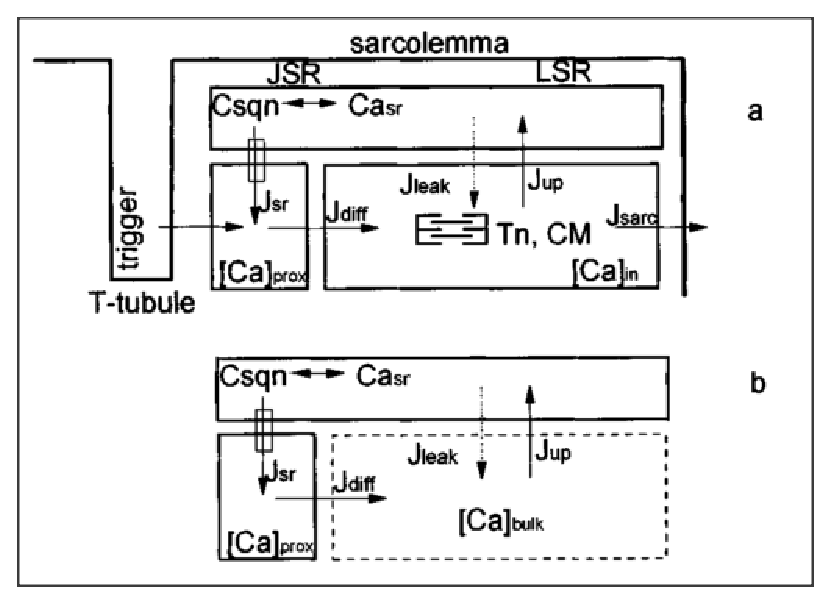
\includegraphics[height=5cm]{./images/Glukhovsky_Ca-cycling.eps}}
\caption{Schematic diagrm of $\Ca$ cycling path in the myocyte}
\label{fig:Glukhovsky_Ca-cycling}
\end{figure}



\section{Priebe-Beuckelmann (1998) - heart failure in human}
\label{sec:priebe-beukelmann_1998}

\citep{priebe1998} build the first model for human heart, with parameters
derived from LR-2 model (Sect.\ref{sec:luo-rudy-phase-2}). In particular, some
selected ionic currents are derived from human data (i.e. $I_\ca, I_\to, I_\Kr,
I_\Ks$, and $I_{K1}$). The other currents ($I_\Na, I_\ncx$, and $I_\NaK$) have
to be adjusted so that the overal result consistent with experimental data in
human. The data is based on experiments at body temperature 37$^\circ$C.

The goal was to investigate the effect of individual current to the AP in human
myocardium.

\subsection{Hypothesis}

A prominent feature of a single myocyte in failing heart is the alteration in
$\Ca$ dynamics and enhanced activity of NCX. These abnormalities can give rise
to arrhythmias. 

Based on experimental data, it's assumed that the kinetics of the following
currents don't change in both normal and HF conditions: $I_\na$, $I_\ca$
\citep{15,16,18}, $I_\to$ \citep{14}. However, the current density of $I_\to$
in HF reduced down to 64\% of the value measured in normal heart.

\subsection{Mathematical analysis}

The time-dependent $V_m$ equation
\begin{equation}
dV_m/dt = -\frac{1}{\Csc} (I_\Na + I_\Ca + I_\to + I_\Kr + I_\Ks + I_\NCX +
I_\NaK + I_\Nab + I_\Cab + I_\stim)
\end{equation}
with $\Csc=1\muF/$cm$^2$. All currents are defined based on 1pF of cell membrane
capacitance, i.e. $\muA/$pF.

\begin{enumerate}
  \item $I_\na$: the formula is the same as Sect.\ref{sec:luo-rudy-phase-2} (as
  \citep{sakakibara1993} suggested that isolated human ventricular myocytes and
  other mammalian species have the same $I_\na$ kinetics) in both groups 
  \item $I_\ca$: the formula is the same as Sect.\ref{sec:luo-rudy-phase-2}, to
  fit the experimental data of $I_\ca$, the equation in the form 
  \begin{equation}
  A \left[\exp(-t/\tau_1) - \exp(-t/\tau_2) \right] + R
  \end{equation} 
  are used; with $\tau_1, \tau_2$ are two time constants; $R$ is basal $[\Ca]$
  level.
\end{enumerate}

\subsection{Analysis}

The main results:
\begin{enumerate}
  \item the APD in failing hearts is longer than in normal hearts. The major
  major underlying mechanism for this prolongation: enhanced activity of NCX,
  slowed diastolic decay of $[\Ca]_i$ transient; and the reduction of inwardly
  rectifying $\K$ current and Na/K-pump current.
  \item the fast and slow components of delayed rectifier $\K$ currents ($\IKr$
  and $\IKs$, respectively) are the two most importance in determining
  repolarization of the membrane potential. Inhibition of $\IKr$ promotes EAD in
  failings, but not in non-failing hearts; where the spontaneous release of
  $\Ca$ can trigger a premature action potential only in failing hearts.
  \item the contribution of $\Ito$ on APD is small in both conditions.
\end{enumerate}



\section{Noble-\ldots-Noble (1998) - guinea pig**}

\citep{noble1998} proposed a guinea ping ventricular myocyte model incorporating
the diad subspace, and other processes such as cellular mechanics, metabolism,
pH dependence, and drug receptor interactions. The model has 27 individual
currents.


\section{Jafri-Rice-Winslow model (1998) - guinea pig}
\label{sec:jafri-rice-winslow}

You are recommended to read LR-2 model first (Sect.~\ref{sec:luo-rudy-phase-2}).
Even though LR-phase 2 model has incorporated many ionic currents and ionic
pumps/exchangers, an important feature in $\Ca$ transient known as gradeness
release of calcium cannot be reproduced. Gradeness means that incremental
release of $\Ca$ from SR occurs in response to the step changes in cytoplasmic
side $\Ca$. It means that \ce{Ca^2+} release from SR is not an all-or-none
process, but incremental increase due to the \ce{Ca^2+} elevation in cytoplasmic 
side. The main explanation for this is that such models lack a
physiologically realistic description of the CICR
(Sect.\ref{sec:local_control}).

$\Ca$ influx doesn't flow direct to the bulk myoplasm, but into a restricted
space known as dyadic space where local elevation is much higher than bulk
myoplasm. This high calcium concentration can triggers the opening of RyRs in
the junctional SR which is in closed proximal to the T-tubule wall. Each local
release site is known as calcium release unit (CRU), and the restricted space is
known as dyadic subspace (diadic subspace) where the calcium concentration is
denoted as $[\Ca]_\ds$. Early experiments estimated of about 5,500 CRUs
(\textcolor{red}{Later data show there are about 20,000 of such microdomain
spaces in rat ventricular cells}). \citep{jafri1998cad} proposed a model to
incorporate this description.  In their model, subspace $[\Ca]$ rises more
rapidly and reaches a higher level (10-30$\muM$) compared to the bulk myoplasmic
$\Ca$ (peak $\sim 1\muM$). During an AP, $\Ca$ transient is similar to
experimental data. Here, both $[\K]$ and $[\Ca]$ are dynamics variables.

\subsection{Hypothesis analysis}
\label{sec:hypothesis-analysis-5}


The schematic diagram of JRW model is shown in
Fig.~\ref{fig:JRW_model}. Compared to Fig. \ref{fig:LR_phase2}; in
this model, $\Ca$ first reach the so-called {\it dyadic subspace}
before it can diffuse into the cytoplasm. The description of the
process is given as follows.
\begin{figure}[hbt]
  \centerline{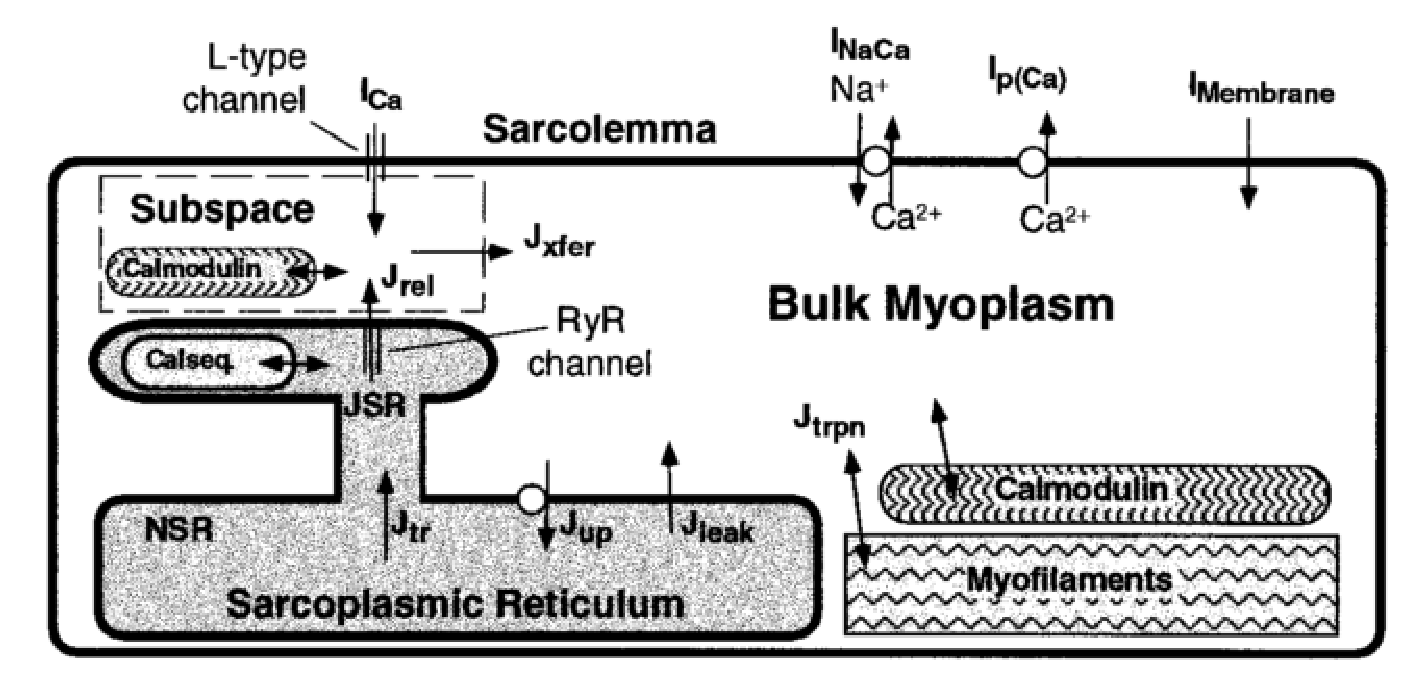
\includegraphics[height=5cm,
    angle=0]{./images/JRW_model.eps}}
\caption{Schematic diagram of calcium dynamics in JRW model}
\label{fig:JRW_model}
\end{figure}

With recent discoveries, we know that in cardiac cells, the major  type of $\Ca$
channels is L-type (or $\alpha_{1C}$) - shortly LCC or aka DHPR (dihydropyridine
receptor). The mechanism of excitation-contraction (EC) coupling is described as
follows. membrane depolarization triggers the opening of LCC, allowing $\Ca$
from extracellular  to diffuse through LCCs triggering $\Ca$ release from
junctional SR via RyR  channels in a process known as CICR. Then, $\Ca$ from the
dyadic subspace quickly diffuse from the subspace into the bulk myoplasm
($J_{efflux}$). After the contraction, $\Ca$ are quickly removed from the
myoplasm via sarcolemma by NCX and ATP-dependent $\Ca$ pumps ($I_\pCa$) or
re-sequestered (reuptake) into NSR by ATPase (SERCA) pump ($J_\SERCA$). The JSR
is refilled by $\Ca$ diffusion from NSR ($J_\rf$).

To balance NSR $\Ca$ content, a non-specific channel is assumed to produce a
leak $\Ca$ current $I_\leak$ from the NSR to the myoplasm. To balance bulk 
myoplasm $\Ca$ content, a background $\Ca$ current across the sarcolemma
($I_\Cab$\footnote{previously notated as $I_\Cab$}) was used.

\subsubsection{Dyadic (diadic) Subspace}
\label{sec:diadic_subspace}


The channels (LCC, RyR) reside in proximity in a specialized
junctional area, where T-tubular system and SR membrane are
separated by a junctional gap forming a dyadic subspace of 12 nm
\citep{frank1990}.

In this model, instead of examining the individual dyadic subspace, all are
lumped into a single pool of volume $V_{ss}$:
\begin{equation}
  \label{eq:778}
  \begin{split}
    V_{ss} = (\text{junctional gap})\times (\text{area of functional
      unit}) \times \\
    (\text{number of functional units})
  \end{split}
\end{equation}
then $V_\ds = 1.485\times 10^{-9}\mu$L (which is about 4 order
smaller than $V_\myo$). \citep{langer1996} (Sect.\ref{sec:Langer-Peskoff_96})
modeled a cleft space as a circular region with the total cleft volume is 0.25$\mum^3$.

Anatomical evidence suggested the ratio LCC:RyR in guinea pig is 1
:5.6~\citep{bers1992}. JRW model use the 4 LCC and 25 RyR per cleft.
Also, \citep{isenberg1995} estimated 5500 L-type $\Ca$ channels per cardiac
myocyte, with cleft dimension $0.3\times 0.3\times 0.012\mum$. So, with total
LCCs is assumed to be 5500, the number of cleft is 5500/4, and thus the total
cleft volume is 1.485$\mum^3$ which is about six time larger than the cleft
being used by \citep{langer1996}. Another assumption is that no spatial $[\Ca]$
gradient exist in the subspace volume, i.e. all RyR see the same $[\Ca]_\ds$.


\subsubsection{Ion concentrations}
%\label{sec:ionic-concentrations-2}


\begin{itemize}
\item standard values for ion concentrations: $[\ce{K}]_o=5.4$mM,
  $[\Na]_o=140$mM, $[\ca]_o=1.8$mM.
  
\item initial values for ion concentrations: $[\ce{K}]_i=143.727$mM,
  $[\Na]_i=10.2042$mM, $[\ca]_i=9.94893\times 10^{-5}$mM,
  \textcolor{red}{new Calcium components}: $[\ca]_\ds=1.36058\times
 10^{-4}$mM, $[\ca]_\jsr=1.17504$mM, $[\ca]_\nsr=1.24891$mM.
  
\end{itemize}

In this model, not only calcium, but also intracellular potassium is
also a dynamic variable.
\begin{itemize}
\item The cytosolic calcium is given in eq.~\eqref{eq:792}.

\item The calcium subspace is given in eq.~\eqref{eq:793}
\item The calcium in junctional SR is given in eq.~\eqref{eq:794}
\item The calcium in network SR is given in eq.~\eqref{eq:795}

\item The potassium in cytosol is given in eq.~\eqref{eq:796}
\end{itemize}

\subsubsection{Ionic currents}
\label{sec:ionic-currents-4}

The ionic currents compared to LR-II (Sect.~\ref{sec:luo-rudy-phase-2}) are
\begin{itemize}
\item the $\Ca$-activated non-specific channel $I_\nsCa$ is not considered
  in the model
  
\item $I_{\ca,\na}$ component is removed; so $I_\ca$ is the only inward current
passing through the channel, eq.~\eqref{eq:779}. 

\item the GHK formulation (using constant field theory) of the $I_\ca $ in
LR-phase 2 model assumes the independent permeability of ions.
  However, recent data show that no monovalent passing when a significant amount
  of $\Ca$ is passing. Thus, a better hypothesis is that $\ce{K+}$ permeability
  $P_{K'}$ is a decrease function of $\Ca$ current,
  ~\eqref{eq:780}. 
  
\item there is a minor change in the maximum conductance of the
time-dependent potassium current $I_{K}$, eq.~\eqref{eq:781}.  
\end{itemize}
There is no change in the fast inward Na current $I_{Na}$,
eq.~\eqref{eq:940}.


\subsubsection{Model DHPR (LCC) kinetics}
\label{sec:model-dhpr-kinetics}

Previous models assuming $\Ca$-binding inactivation is instantaneous. However,
there were some evidence suggested that this inactivation is time-dependent. So,
a mode-switching approach was used \citep{imredy1994mcs}. Here, LCC is
represented using Markov-chain model based on the concept of mode-switching
(Sect.\ref{sec:LCC_Jafri1998}). When the channel is open, the $\Ca$ flux is
formulated using GHK equation, eq.\ref{eq:779}.

\subsubsection{Model RyR kinetics}
\label{sec:model-ryr-kinetics}

RyR adaptation has been suggested else where \citep{gyorke1993ryr}. Several
models has been proposed using adaptation \citep{cheng1995, keizer1996rra}
 JRW use RyR model modified from Keizer-Levine model
(Sect.~\ref{sec:keizer-levine-1996}) in which the adaptation is
$\Ca$-independent, as shown in Fig.~\ref{fig:Keizer_Levine_RyR}, with
\begin{itemize}
\item original rate constants are designed with the assumption that
  RyR face cytosolic calcium with peak $[\Ca]_i$ to $1\muM$. However,
  with the new idea of RyR facing the subspace which can experience a
  much higher calcium concentration and can change more rapidly, the
  rate constants are modified to adjust channel sensitivity to
  $[\Ca]_\ds$ which can excess 10$\muM$.

\item A faster adaptation rate with physiological level of $\Mg$
\citep{valdivia1995} has been incorporated by changing $k^+_c$. 

\item The bilayer experiment in \citep{gyorke1993ryr} was carried out at room
temperature (25$^\circ$C). Thus, values were adjusted to match the condition
37$^o$C in cardiac ventricular cells. 

\item The fraction of RyR opening at rest is chosen as 0.0012
\end{itemize}


\begin{figure}[hbt]
  \centerline{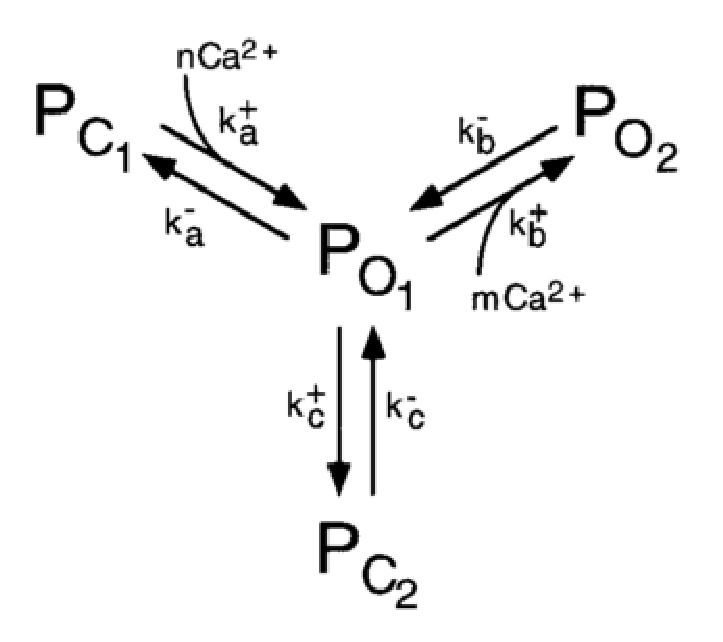
\includegraphics[height=5cm,
    angle=0]{./images/KeizerLevine_model.eps}}
  \caption{Schematic diagram of RyR. The model has 2 open states $O_1,
    O_2$ and 2 closed states $C_1, C_2$. Transitions from $C_1$ to
    $O_1$, and $O_1$ to $O_2$ are $\Ca$-dependent.}
\label{fig:Keizer_Levine_RyR}
\end{figure}



\subsubsection{Buffering}
\label{sec:buffering-1}


It's important to know that almost 90\% of the total $\Ca$
released during a contraction (CICR process) is sequestered by
$\Ca$ buffers \citep{berlin1994iccb}.
\textcolor{red}{ In cardiac cells, those buffers can be mobile buffer
  (Calmodulin), stationary buffers (troponin C and myosin)}.
In junctional SR\footnote{SR luminal = inside SR}, calsequestrin (CSQ2) is
the most abundant $\Ca$-binding protein.  $\Ca$ ions quickly
bind to buffers, e.g. the calmodulin (CaM) in the subspace and myoplasm, or
troponin in the myoplasm for excitation-contraction purpose, or
calsequestrin in the JSR. A detail of different buffers is discussed
in Sect.~\ref{sec:buffers-calcium}.


\begin{equation}
  \label{eq:228}
  B + \ce{Ca^2+ <=>[k_{on}][k_{off}] CaB}
\end{equation}

Typically, the kinetics of binding is fast compared to $\Ca$ release, then
eq.~\eqref{eq:228} remains close to equilibrium during the $\Ca$ transient. As a
result, \textcolor{blue}{rapid buffering is a common assumption to approximate
 calcium-bound to buffer} $[\CaB]$ (Sect.~\ref{sec:slow_rapid-bufferings}). Thus
 we can use Michaelis-Menten-type equation. Otherwise, we need to solve ODE
 based on reaction kinetics.


Like previous models, the effect of myosin was ignored (due to small
contribution, e.g. about 2.3\% saturated during $\Ca$
transient). \textcolor{red}{Except for high- and low-affinity troponin,
  Calsequestrin and Calmodulin are considered as fast buffer}.
In JRW model, both low- and high-affinity sites of
$\Ca$ for troponin are used.  So, we need to have 2 ODEs for $[\CaHtrpn]$ and
$[\CaLtrpn]$, eq.~\eqref{eq:31} and eq.~\eqref{eq:32}.

\begin{itemize}
\item Buffering in the network SR was neglected.

\item Buffering factor in JSR is CSQN, eq.~\eqref{eq:791}
\item Buffering factor in subspace is CMDN, eq.~\eqref{eq:791}
\item Buffering factor in myoplasm is CMDN, assuming the same kinetics
  with the one in subspace, eq.~\eqref{eq:791}, and high-affinity
  troponin (HTRPN) + low-affinity troponin (LTRPN).

\item The flux in the directive of forming Ca$\cdot$Trpn compound is
  given in eq.~\eqref{eq:229}.
\end{itemize}

\subsubsection{Fluxes}
\label{sec:fluxes}

In this multi-compartment model, besides the ionic currents, we also
have the ionic fluxes, as shown in Fig.~\ref{fig:JRW_model}, that
affect the concentrations of dynamics variables.
\begin{enumerate}
\item $J_\xfer$ (or later known as $J_\xf$) = calcium diffuse
  from subspace to bulk myoplasm, eq.~\eqref{eq:789}.
\item $J_\rel$ (or later known as $J_\ryr$) = calcium diffuse from JSR
  to subspace, eq.~\eqref{eq:785}.
\item $J_\tr$ (or later known as $J_\rf$) = calcium translocate from
  NSR to JSR, eq.~\eqref{eq:790}
\item $J_\up$ (or later known as $J_\serca$) = calcium re-uptake by
  SERCA pumps, eq.~\eqref{eq:788}.
\item $J_\leak$ = constant calcium leak to balance the calcium
  re-uptake at resting state, eq.~\eqref{eq:787}
\end{enumerate}



\subsection{Mathematial model}
\label{sec:mathematial-model}

The dynamics of potential is based on
\begin{equation}
  \label{eq:1264}
  \begin{split}
    \frac{dV_m}{dt} = \frac{-1}{\Csc}\left(I_\na + I_\ca + I_\k +
      I_{K1}
      + I_\Kp + I_\NaCa + I_\NaK \right.\\
    \left. + I_\nsCa + I_\pCa + I_{\ca,\k} + I_\Cab + I_\Nab \right)
  \end{split}
\end{equation}
with $\Csc =1\muF$/cm$^2$.

\subsubsection{Ionic and pumps/exchanges currents}
\label{sec:ionic-pumps-curr}

\begin{enumerate}
\item fast inward Na current $I_{Na}$ (the same as LR-phase 2)
\item $I_\ca $ (use GHK equation~\eqref{eq:544})
  \begin{equation}
    \label{eq:779}
    I_\ca  = \overline{P_\ca } y (O + O_\ca )z^2_\ca \frac{V_mF^2}{RT}
    \frac{0.341[\ca]_o - 0.001\exp[\frac{z_\ca V_mF}{RT}]}{ 1-
      \exp[\frac{z_\ca V_mF}{RT}]}
  \end{equation}
  with $\overline{P_\ca }=54\times 10^{-4}$ cm/s is maximum
  permeability; $y$ is $V_m$-inactivation gate which is modeld using
  Hodgkin-Huxley type (which can inactivate the channel independently of the
  states); $(O+O_\ca) $ is the fraction of open channel (or open probability or
  number of open channels, depending on the interpretation); $z_\ca =2$ the valence of $\Ca$. The last expression is the
  {\it electrochemical driving
    force}\footnote{electrochemical driving force = difference
    between membrane potential and equilibrium potential. The current
    through a channel is the product of the channel conductance and
    the electrochemical driving force.}
  for L-type $\Ca$ current (see eq.~\eqref{eq:360}).
  
  \begin{equation}
  \begin{split}
  y_\infty = 0.02 + \frac{1}{1+ e^{(V_m+55)/7.5}} + \frac{1}{1+e^{(V_m-21)/6}}
  \\
  \tau_y = 0.02 + \frac{0.04}{1 + e^{(V_m+30)/9.5}}
  \end{split}
  \end{equation}
  
  \begin{framed}
  REMEMBER:  The number 0.341 reflects the activity coefficient of $\Ca$ at the
    outer opening of the cell, and 0.001 reflects the product of the
    activity coefficient of $\Ca$ at the mouth of the DHPR channel and
    the $[\Ca]_\ds$. 
  \end{framed}

\item The K current via LCC $I_{\ca,\k}$
  \begin{equation}
    \label{eq:784}
    I_\CaK = P'_K y (O + O_\ca ) z^2_\ca \frac{z_\k V_mF^2}{RT}
    \frac{0.341[\ce{K}]_o - [\ce{K}]_i\exp[\frac{z_\k V_mF}{RT}]}{ 1-
      \exp[\frac{z_\k V_mF}{RT}]}
\end{equation}
with the permeability of \ce{K+} via LCC.
\begin{equation}
  \label{eq:780}
  P_{K'} = \frac{\overline{P_K}}{1+\frac{I_{Ca,max}}{I_{Ca,half}}}
\end{equation}
where $\overline{P_{K}}=1\times 10^{-7}$ (cm/s) is the permeability of
K in the absence of $\Ca$ current;
$I_{Ca,half}=-0.458$($\muA$/$\muF$) is the level of $\Ca$ current
that reduce half of the permeability of $P_{K'}$. The maximal L-type
current $I_{Ca,max}$ is derived from constant field theory
\begin{equation}
  \label{eq:782}
  I_{Ca,max} = \overline{P_\ca }z^2_\ca \frac{V_mF^2}{RT}
  \frac{0.341[\ca]_o-0.001\exp[\frac{z_\ca
      V_mF}{RT}]}{1-\exp[\frac{z_\ca V_mF}{RT}]}
\end{equation}

\item time-dependent K current $I_K$ (similar to LR-phase 2, except a
  minor change in the maximum conductance)
  \begin{equation}
    \label{eq:781}
    \overline{g_{K}} = 0.1128 \sqrt{\frac{[\ce{K}]_o}{5.4}}
  \end{equation}

NOTE: The idea of ~\citep{zeng1995} has not been considered in the model, where
$I_\k$ is composed of 2 components:
  $I_\Kr$ (faster deactivation kinetics) and $I_\Ks$ (slower). So, at high
  pacing rates (e.g. 4Hz), there is not enough time for $I_\Ks$ to return to
  closed state, i.e. $I_\Ks$ achieves higher resting open probabilities at
  higher pacing frequencies.

\item time-independent K current $I_{K1}$ (the same as LR-phase 2)

\item plateau K current $I_{Kp}$ (similar to LR-phase 2, except a
  minor change in the maximum conductance)
  \begin{equation}
    \label{eq:783}
    \overline{g_{Kp}} = 0.00828 \text{(mS/$\muF$)}
  \end{equation}

\item the \ce{Na+}/$\Ca$ exchanger $I_\NCX$ (similar to
  LR-phase 2 (eq.~\eqref{eq:770}), except a minor change in the
  parameters): scaling factor ( $k_\NCX = 5000$ ($\muA$/$\muF$)

\item the \ce{Na+}/\ce{K+} exchanger $I_{Na/K}$ (similar to LR-phase
  2, except a minor change in maximum current $\overline{I_{Na/K}} =
  1.3$ ($\muA$/$\muF$))

\item the $\Ca$-activated non-specific channel $I_\nsCa$
  (\textcolor{red}{removed from the model})

\item the sarcolemmal $\Ca$ pump $I_\pCa$ (the same as
  LR-phase 2)

\item the Ca background current $I_\Cab$ (similar to LR-phase 2,
  except a minor change in the maximum conductance
  $\overline{g_\Cab} = 0.006032$ mS/$\muF$)

\item the Na background current $I_\bNa$ (the same as LR-phase 2)
\end{enumerate}


\subsubsection{Model DHPR and RyR}
\label{sec:model-dhpr-ryr}


\begin{enumerate}
\item model DHPR: The fractions of LCCs in each state are represented
  by 12 ODEs.
    \begin{equation}
      \label{eq:777}
      \begin{split}
        \frac{dC_0}{dt} &= \beta C_1 + \omega C_{Ca0} -
        C_0(4\alpha+\gamma) \\
        \frac{dC_1}{dt} &= 4\alpha C_0 + \frac{\omega}{b}C_{Ca1} +
        2\beta C_2 - C_1(\beta + 2\alpha+a\gamma) \\
        ...
      \end{split}
    \end{equation}
    with $a=2.0, b=2.0$.

    In this new interpretation, the mode switching occur with some
    delay after channel activation; and the switching to mode normal
    is not instantaneously when calcium concentration falls.

%     The transition rate ($[ms^{-1}]$) for $I_\ca $
The $V_m$-dependent activation is incorporated through the rate constants
$\alpha$ and $\beta$ which are increasing and decreasing function of $V_m$,
respectively. 
    \begin{equation}
      \label{eq:763}
      \begin{split}
        \alpha = 0.4\exp[\frac{V_m+12}{10}] \;\;;
        \beta = 0.05 \exp[-\frac{V_m+12}{13}] \\
        \alpha'=a \times \alpha \;\;;
        \beta' = \frac{\beta}{b} \\
        \gamma = 0.1875 [\ca]_{ss} \;\;;
        \omega = 0.01 \text{ ms}^{-1} \\
        f = 0.3 \text{ ms}^{-1} \;\;;
        g = 2.0 \text{ ms}^{-1} \\
        f' = 0.0 \text{ ms}^{-1} \;\;;
        g' = 0.0 \text{ ms}^{-1} \\
      \end{split}
    \end{equation}
    with $\alpha, \beta$ are $V_m$-dependent activation gates. 
    
\item model RyR

....

\end{enumerate}


\subsubsection{Calcium + Potassium concentrations}
\label{sec:calcium-+-potassium}


There are 10 different ODEs to specify the time rate of changes in
[$\Ca$]:
\begin{enumerate}
\item $c_\myo$: we assume L-type current $I_\ca$ only flow into the subspace
  \begin{equation}
    \label{eq:792}
    \begin{split}
      \frac{d[\ca]_\myo}{dt} = \beta_\myo \left( J_\leak + J_{efflux} -
        J_{serca} - J_{trpn} - \right. \\
        \left. \frac{A_{cap}}{z_\ca V_\myo F}(I_\Cab +
        I_\pCa - o_\NCX\times I_\NCX) \right)
    \end{split}
  \end{equation}
  with $z_\ca =2$ (valence of $\Ca$), $o_\NCX=2$ (the number
  of Ca ion extruded in Na/Ca exchanger). The influx calcium current
  is negative by convention in electrophysiology. So, for it to make
  positive contribution to cytosolic calcium, we need to change the
  sign.

\item $c_\ds$
  \begin{equation}
    \label{eq:793}
    \frac{d[\ca]_\ds}{dt} = \beta_\ds \left( J_\rel 
      - J_{efflux}\frac{V_\myo}{V_\ds} - \frac{A_{cap}}{z_\ca V_\ds F}I_\ca   \right)
  \end{equation}
\item $c_\jsr$
  \begin{equation}
    \label{eq:794}
    \frac{d[\ca]_\jsr}{dt} = \beta_\jsr \left( J_\rf - J_\rel\frac{V_\ds}{V_\jsr}\right)
  \end{equation}
\item $c_\nsr$
  \begin{equation}
    \label{eq:795}
    \frac{d[\ca]_\nsr}{dt} =
    (J_{serca}-J_\leak)\frac{V_\myo}{V_\nsr} - J_\rf \frac{V_\jsr}{V_\nsr}
  \end{equation}

\item $[\CaLtrpn]$: [$\Ca$] bound to low-affinity
  troponin-binding sites
  \begin{equation}
    \label{eq:31}
    \frac{d[\CaHtrpn]}{dt} = k^+_\htrpn [\Ca]_\myo (c^T_\htrpn-[\CaLtrpn])
    - k^-_\htrpn [\CaHtrpn]
  \end{equation}
\item $[\CaHtrpn]$:  [$\Ca$] bound to high-affinity
  troponin-binding sites
  \begin{equation}
    \label{eq:32}
    \frac{d[\CaHtrpn]}{dt} = k^+_\htrpn [\Ca]_\myo (c^T_\htrpn-[\CaLtrpn])
    - k^-_\htrpn [\CaHtrpn]
  \end{equation}
% \item $c_{csqn}$:  [$\Ca$] at calsequestrin in JSR

% \item $c_{cmdn, myo}$: [$\Ca$] at calmodulin in the myoplasma

% \item $c_{cmdn, ds}$: [$\Ca$] at calmodulin in the dyadic
%   subspace

\item $[\ce{K}]_i$:
  \begin{equation}
    \label{eq:796}
    \frac{d[\ce{K}]_i}{dt} = -(I_K+I_{K1}+I_{Kp}+I_{ns,K} -
    2I_{Na/K}+I_\CaK) \frac{A_{cap}}{z_\k V_\myo F}
  \end{equation}
  the minus is added in the front the K flow inward are negative while
  contribution is expected to be positive.
\end{enumerate}

\subsubsection{$\Ca$ fluxes}
\label{sec:calcium-fluxes}

Correspondingly, there are 6 $\Ca$ fluxes
\begin{enumerate}
\item the flux $J_\rel$ of $\Ca$ release from JSR via RyR to the
  dyadic subspace (thus aka $J_{ryr}$)
  \begin{equation}
    \label{eq:785}
    J_\rel = J_{ryr} = v_\rel\times (RyR)_{open}\times ([\ca]_\jsr - [\ca]_\ds)
  \end{equation}
  with $v_\rel$ is the maximum flux (or flux for a single RyR) when
  all RyR open, $(RyR)_{open}$ is the fraction of RyR open (or the
  total number of RyR open, respectively). 
  \begin{equation}
    \label{eq:786}
    (RyR)_{open} = P_{O1} + P_{O2}
  \end{equation}

  \begin{framed}
    NOTE: The passive flux from A into B is defined as $J=v.(c_A-c_B)$
    with $v$ is the transfer rate of the species from A to B
    compartment, then we can assign $dc_B/dt=J$. Noting that
    $d(c_A.V_A)/dt=-d(c_B.V_B)/dt$, then $dc_A/dt =
    -\frac{dc_B}{dt}.\frac{V_B}{V_A}$.
  \end{framed}
\item the flux $J_{efflux}$ ($J_{xfer}$) of $\Ca$ from dyadic
  subspace diffuse into the cytoplasm
  \begin{equation}
    \label{eq:789}
    J_{efflux} = \frac{1}{\tau_{efflux}} ([\ca]_\ds-[\ca]_\myo)
  \end{equation}
  with $\tau_{efflux}=3.125$ms (the time constant for transfer from DS
  to MYO)

\item the leak $J_\leak$ from NSR to cytoplasm is a linear function
  \begin{equation}
    \label{eq:787}
    J_\leak = v_\leak ([\ca]_\nsr - [\ca]_\myo)
  \end{equation}
  with $v_\leak$ is the leak rate constant; $[\ca]_\myo$ is a
  different notation of $[\ca]_i$

\item the uptake $J_{serca}$ ($J_{up}$) from myoplasm back to NSR is
  modeled using simple Michaelis-Menten approach with 2 binding sites
  (Sect.~\ref{sec:mich-ment-appr})
  \begin{equation}
    \label{eq:788}
    J_{serca} = v_{serca} \frac{([\ca]_\myo)^2}{K^2_{m,serca}+([\ca]_\myo)^2}
  \end{equation}
  with $v_{serca}$ is the maximum pump rate, $K_{m,serca}$ is the
  half-saturation constant for the SERCA pump. The major difference
  from that in LR-phase2 is the Hill coefficient which is now set to
  2, and is consistent with experimental finding of 2 calcium-binding
  sites (Lyton {\it et al.}, 1992).

\item the flux $J_\rf$ ($J_{tr}$) from NSR to JSR
  \begin{equation}
    \label{eq:790}
    J_\rf = \frac{1}{\tau_\rf} ([\ca]_\nsr-[\ca]_\jsr)
  \end{equation}
  with $\tau_\rf = 34.48$ ms. 

\end{enumerate}

\subsubsection{Buffering}
\label{sec:buffering-4}

\begin{enumerate}
\item the rapid buffering (by Calmodulin and Calsequestrin) is
  assumed; then the scaling factor $\beta_\jsr$ (calsequestrin in
  JSR), $\beta_\ds$ (Calmodulin in dyadic subspace), $\beta_\myo$
  (Calmodulin in myoplasm)
  \begin{equation}
    \label{eq:791}
    \begin{split}
      \beta_\jsr =
      \frac{1}{1+\frac{[\CSQN]_{tot}K_{m,\CSQN}}{(K_{m,\CSQN}+[\ca]_\jsr)^2}}
      \\
      \beta_\ds =
      \frac{1}{1+\frac{[CMDN]_{tot}K_{m,CMDN}}{(K_{m,CMDN}+[\ca]_\ds)^2}}
      \\
      \beta_\myo = \frac{1}{1+\frac{[CMDN]_{tot}K_{m,CMDN}}{(K_{m,CMDN}+[\ca]_\myo)^2}}
    \end{split}
  \end{equation}
with $K_{m,\CSQN}=0.8$mM, and $K_{m,\CMDN}=2.38\muM$. 

\item the slow buffering (by high-affinity and low-affinity binding
  sites at Troponin) $J_{trpn}$.
  \begin{equation}
    \label{eq:229}
    \begin{split}
      J_{trpn} = k^+_{htrpn} c_\myo (c^T_{htropn} - [\CaHtrpn]) -
      k^-_{htrpn} [\CaHtrpn] + \\
      k^+_{ltrpn} c_\myo (c^T_{ltrpn} -
      [\CaLtrpn]) - k^-_{ltrpn} [\CaLtrpn]
    \end{split}
  \end{equation}
  with $c^T_{ltrpn}, c^T_{htrpn}$ is the total myoplasmic troponin
  low-affinity site concentration, and high-affinity site
  concentration, respectively. $k^+_{htrpn}$ is the ``on'' rate
  constant for troponin high-affinity sites, $k^-_{ltrpn}$ is the
  ``off'' rate constant for troponin low-affinity sites.
  \begin{itemize}
  \item The fist term in eq.~\eqref{eq:229} describes the rate of
    removing free $\Ca$ due to their binding to troponin
    high-affinity $\Ca$-binding sites.
  \item The second term describes the rate of leaving from these sites
  \item The thirst term describes the rate of removing free $\Ca$
    due to their binding to troponin low-affinity $\Ca$-binding
    sites.
  \item The fourth ...    
  \end{itemize}

\end{enumerate}

\subsection{Numerical methods}
%\label{sec:numerical-methods}

The full set of 30 ODEs was solved using Merson Modified Runge-Kutta
4-th order Adaptive Step Algorithm (Sect.\ref{sec:rkm}), with
\textcolor{red}{ maximum time step-size of 0.1 ms and maximum error
  tolerance of $10^{-6}$}. To equalize the contribution of errors from
  all variables, they were normalized by divided a weighted factors:
\begin{itemize}
\item divide $V_m$ by 100 mV
\item divide $[\Na]_i$ by 5 mM
\item divide $[\ce{K}]_i$ by 140 mM
\item divide $[\ca]_i$ by 0.001 mM
\item divide $[\ca]_\nsr$ by 2mM
\item divide $[\ca]_\ds$ by 0.001 mM
\item divide $[\ca]_\jsr$ by 20 mM
\item all other variables were given weights of 1.0
\end{itemize}

Action potentials were initiated by a 0.1 mA/$\muF$ current
injected for $0.5$ ms. 



\subsection{Analysis}
\label{sec:analysis-12}

The model is then used to study (using AP)
\begin{itemize}
\item the effect of RyR adaptation and SR load on cardiac AP
\item interplay of RyR adaptation and SR load on frequency-dependent
  aspects of the cardiac $\Ca$-transient.
\item effect of caffeine
\end{itemize}

The L-type current reaches the peak at 6.46$\muA/muF$ within 2ms of the
stimulus. The current quickly decreases when $V_m$ reaches the peak; then a
secondary reduction due to $\Ca$ inactivation (after $\sim 30$ms), and finally
going back to zero due to $V_m$-dependent inactivation (after $\sim 100$ms).
In Fig.\ref{fig:Jafri1998_Fig5}(B), $I_\ca$ with depleted SR in dotted line
showed a higher current, which replicate the effect of removing $\Ca$
inactivation mechanism from subspace calcium; which is consistent with the
experimental finding of \citep{grantham1996}. Using AP, the peak $V_m$ can reach
50.4mV. The shorter APD and lower plateau range in normal condition compared to
that without SR calcium (as the effect of calcium inactivation to LCC was removed).

The subspace has a higher level of calcium $[\Ca]_\ds$ (peak 22.2$\muM$) with
faster dynamics than global calcium $[\Ca]_\myo$ (peak about 1$\muM$),
Fig.\ref{fig:Jafri1998_Fig5}. With caffeine emulation (pacing the cell at 1Hz at
low $[\Ca]_o=0.1$mM (normal is 1.8mM), and set $P_{o,\ryr}=0.8$), SR was
depeleted after 10sec. NOTE: $P_{o,\ryr}=P_{o1}+P_{o2}$. Without SR calcium,
$[\Ca]_\ds$ can reach about 0.5$\muM$.

\begin{figure}[hbt]
  \centerline{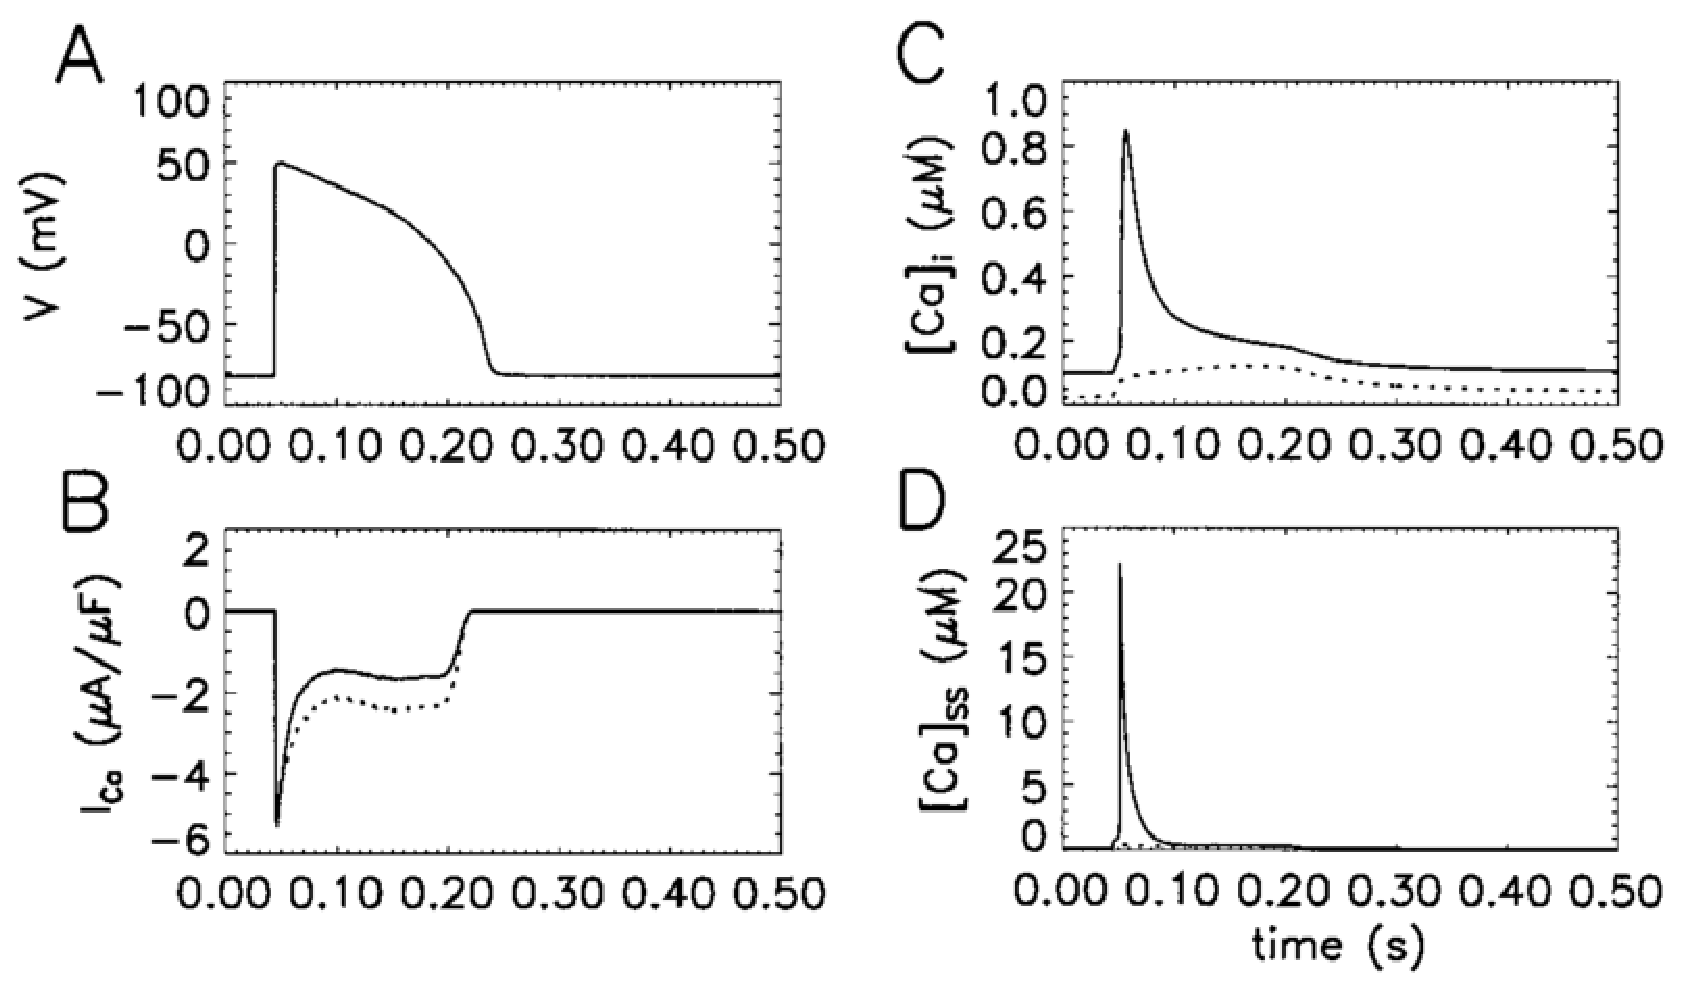
\includegraphics[height=5cm]{./images/Jafri1998_Fig5.eps}}
  \caption{Simulated result using AP protocol.}
  \label{fig:Jafri1998_Fig5}
\end{figure}

$\Ca$ transient can rise to 0.84$\muM$, from resting 0.1$\muM$. Without SR
calcium, the $\Ca$ transient can rise to 0.12$\muM$ from 0.02$\muM$.
Adaptation was tested in which the rate to the adapted state ($k_c^=0.018$
ms$^{-1}$) is replaced by zero value, and using fast adaptation,
Fig.\ref{fig:Jafri1998_Fig6.7}(I).
The removal of adaptation doesn't affect the opening, the closing is delayed
slightly, resulting a small interval during which $P_{o,\ryr}$ retaining at high
level. So, strong adaptation can cause a latency in calcium transient and
smaller amplitude (due to the delayed and smaller $P_{o,\ryr}$).  When more
channels in the adapted state $P_{C2}$, less fraction of channels in C1
available to make the transition from $P_{C1}$ to $P_{O1}$.
Also, the amount of SR $\Ca$ released is about 28\% of the
total SR calcium, with $[\Ca]_o=1.8$mM, which is closed to the experimental
result 35\% \citep{bassani1995fsr}.

\begin{figure}[hbt]
  \centerline{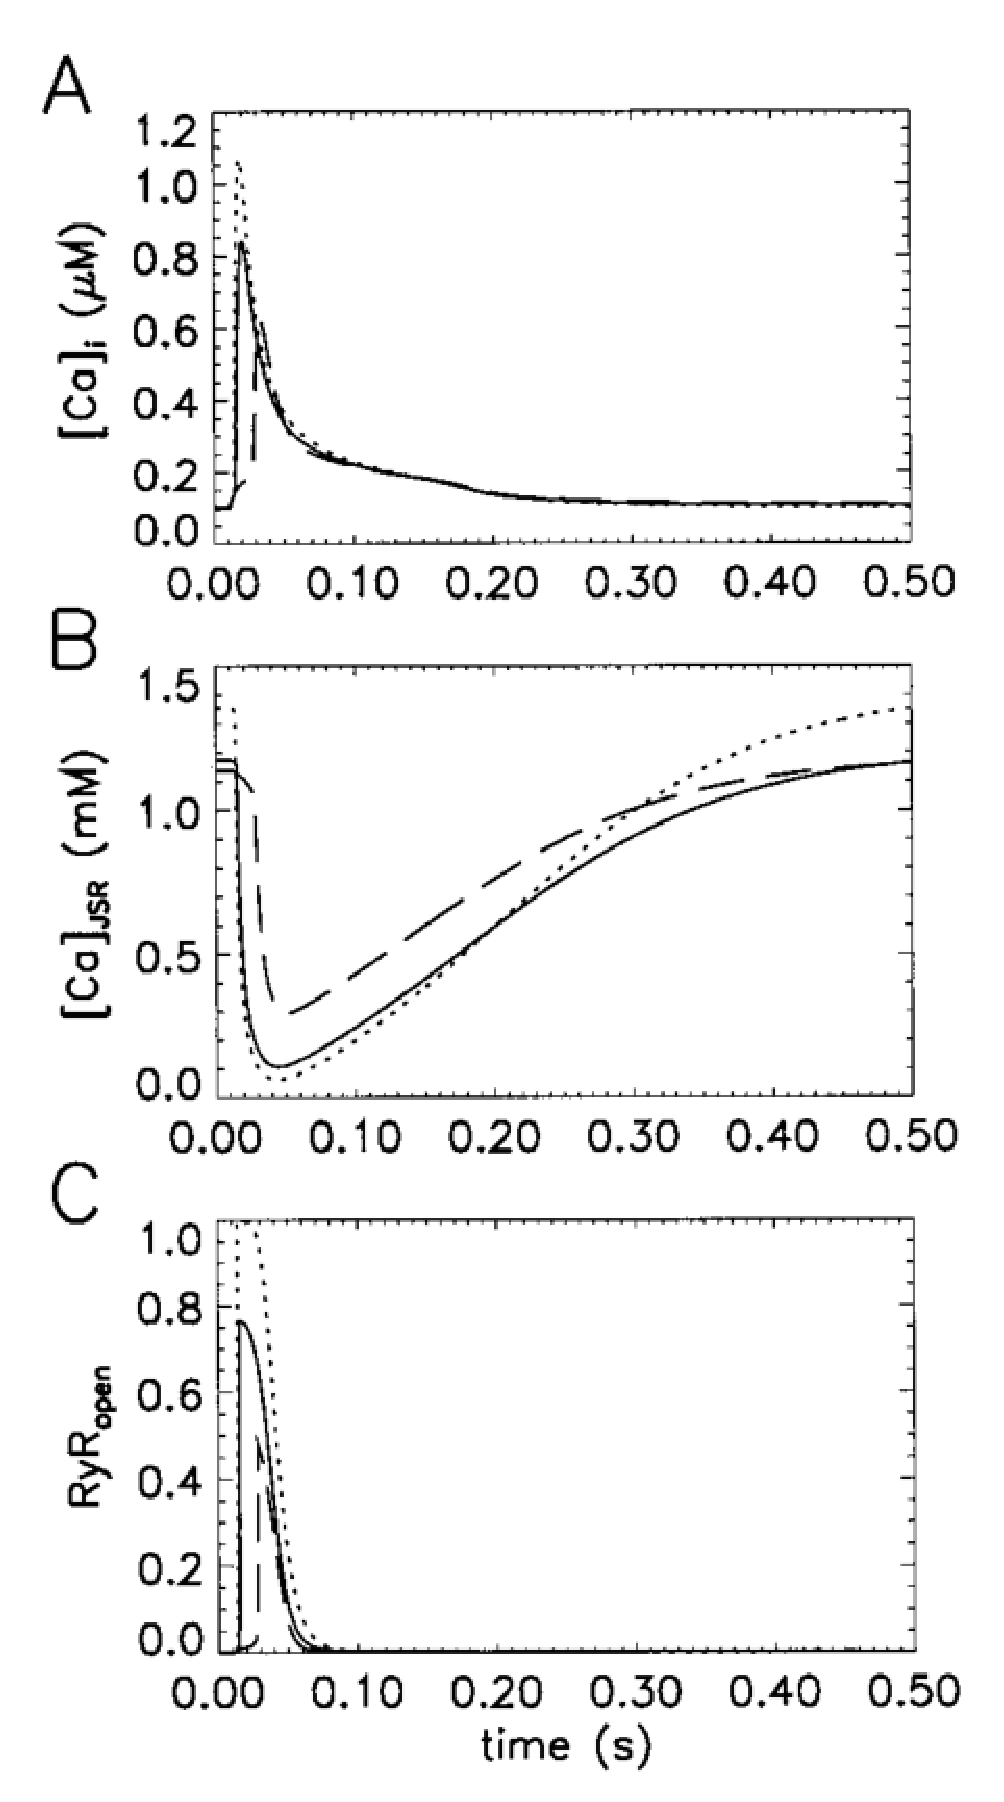
\includegraphics[height=5cm]{./images/Jafri1998_Fig6.eps};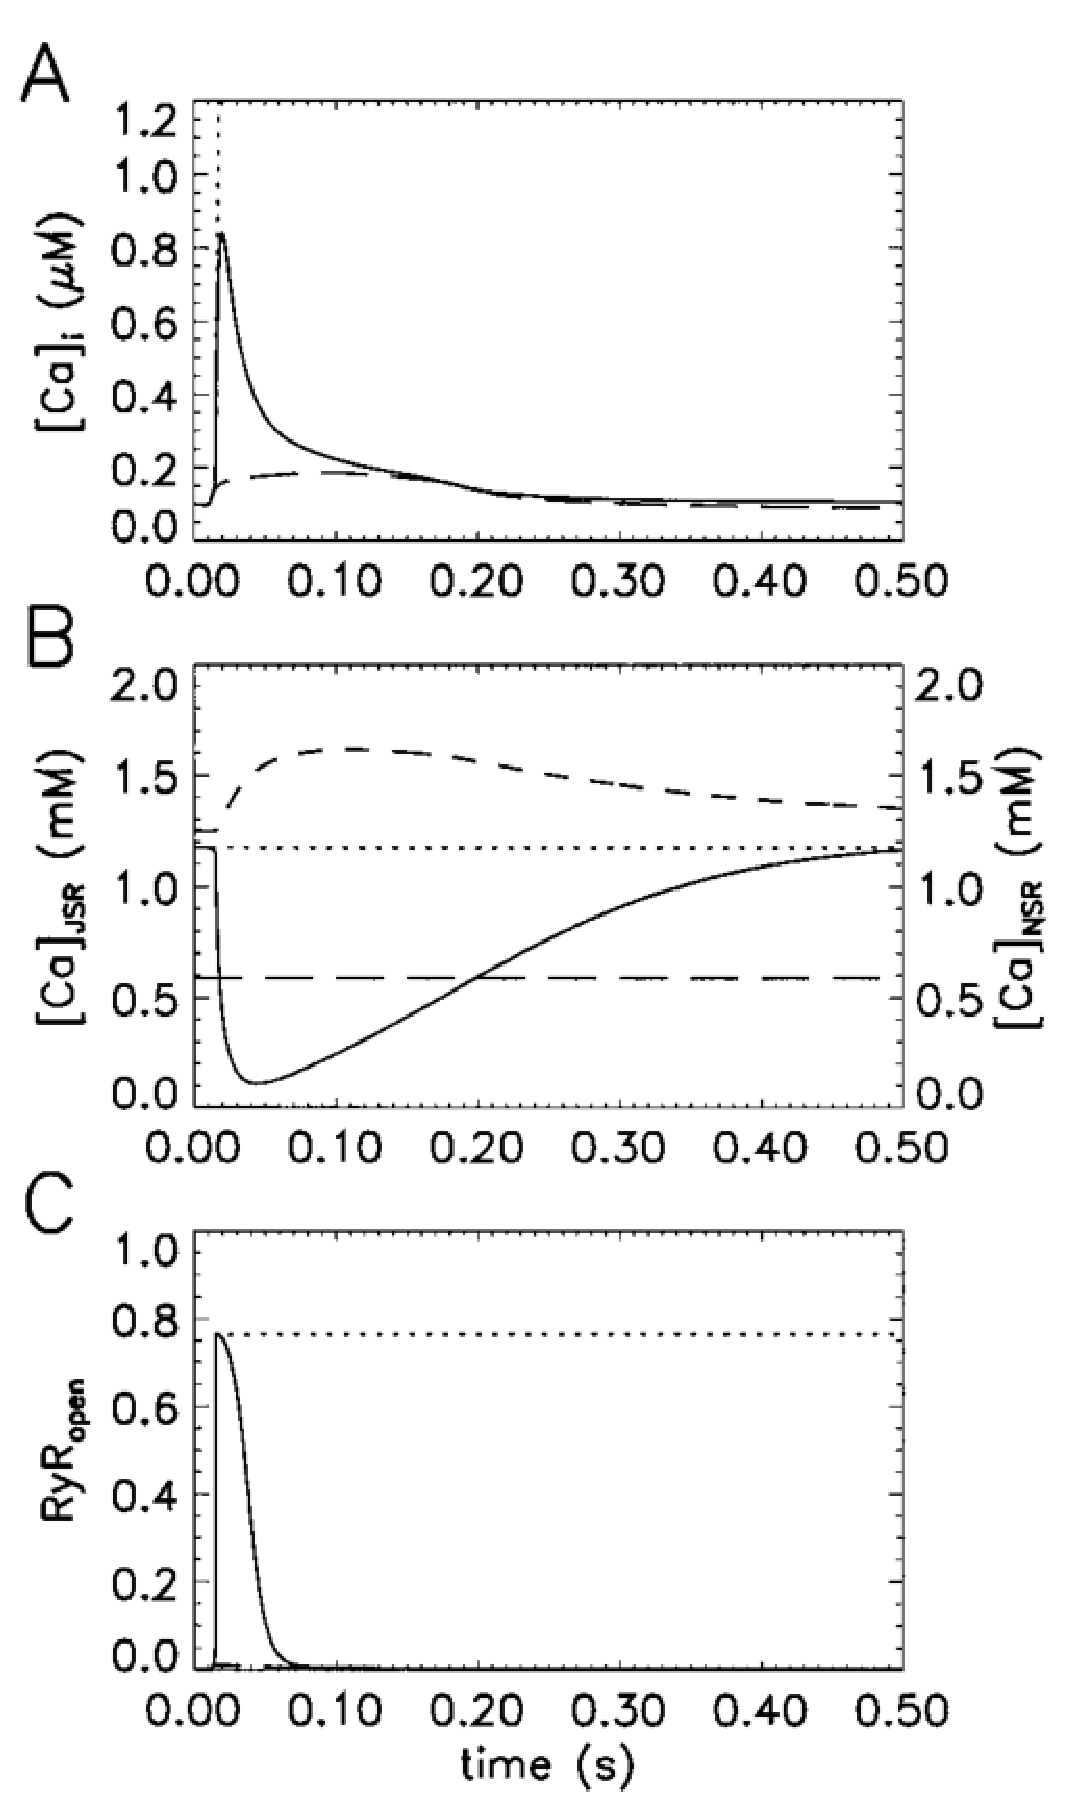
\includegraphics[height=5cm]{./images/Jafri1998_Fig7.eps}}
  \caption{(I) solid line = control simulation (with adaption); dotted line = no
  adaptaion; dashed line = fast adaptaion ($k_c^+=0.072$ms$^{-1}$.
  (II) The role of SR depletion in terminating $\Ca$ release}
  \label{fig:Jafri1998_Fig6.7}
\end{figure}



Jafri-Rice-Winslow model is the first whole-cell model to depart from
the Hodgkin-Huxley approach, as the channel kinetics are represented
by a Markov chain model, e.g. L-type channel and RyR. In a dyadic
subspace, anatomial evidence suggest the ratio RyR:LCC about 5.6:1 in
guinea-pig (Bers, Stiffel, 1992). Other ionic currents was from LR-2 model.
High gain can be simulated in the model. 
  
JRW model is still a deterministic model with all dyadic  subspaces are lumped
into a single one, and thus the number of RyR and LCC channels in each states
can be approximated using ODEs, i.e. fraction of channels in each state.
Nevertheless, JRW model can serve as a basis of network models to understand
early after depolarization (EAD), which might be responsible for certain
arrhythmias.
As the single diad subspace is an assemble average of a large number of diad
subspace, it makes the model is still a common-pool model, i.e. the model expose
all-or-none $\Ca$ release; which is not realistic. Even though LR-2 model can
produce gradeness release, the mechanism of CICR is not corrected, where RyR
should see subspace $\Ca$, not bulk myoplasm.
As pointed out by \citep{stern1992tec}, the graded release would be the
recruitment of several CRUs. So, a proper model should incorporate a significant
number of CRUs in the simulation.


\section{Winslow et al. (1999) - canine}
\label{sec:winslow-et-al}

~\citep{winslow1999} model is based on~\citep{jafri1998cad}
(Sect.~\ref{sec:jafri-rice-winslow}) with some changes in parameters' values,
and adding new components.
This is the first model to study electrical properties for canine, targeting to
canine midmyocardial ventricular cells under HF condition.
In addition to parameters adjusted for canine, a thermodynamics model of SERCA
pump was incorporated (Sect.~\ref{sec:shannon-et-al}), rather than using classic
Hill-equation.

In failing hearts,
\begin{itemize}
\item both SERCA pumps and phospholamban (PLN) are decreased by 28\%
  on average. As a result, time constant of calcium uptake is
  prolonged (576$\pm$13 vs. 282$\pm$30ms in control canine
  midmyocardial ventricular myocyte), i.e. uptake rate is reduced
  $\sim 50\%$ (in end-stage heart failure).

\item NCX proteins is increased by 104\%, as NCX mRNA level
(Sect.\ref{sec:mRNA-level-2-protein-expression}) increases $\sim$55\% to 79\%,
and NCX protein levels increase 36\% to 160\%. However, the role of NCX in heart
failure was not well
  understood.

\item $I_{K1}$ current density reduces $\sim$50\% (in human), with
  magnitude reduced $\sim 40\%$ (in canine)

\item $I_{to1}$ current density (calcium-independent transient outward) is
reduced by $\sim$75\% in subepicardial and $\sim$40\% in midmyocardial
  ventricular cells (both in human), while unchanged in subendocardial
  ventricular cells; with magnitude reduced by $\sim 70\%$ (in
  canine). 
\end{itemize}

Based on data of~\citep{ORourke1999}, Winslow {\it et al.}  created a
model to study how the different parameters ($I_{to1},I_{K1}$, the
upregulation of NCX and downregulation of SERCA) affect to the
calcium dynamics (e.g. reduce amplitude, altered shape, and slower
relaxation of $\Ca$ transient).

\subsection{Hypothesis analysis}
\label{sec:hypothesis-analysis-15}


\subsubsection{Ion concentrations}
%\label{sec:ionic-concentrations-4}

All ion concentrations are examined ($\Ca$, $\Na$, and $\K$).

$[\K]_o=4.0d3 \muM$; $[\Na]_o=138\muM$; $[\Ca]_o=2d3\muM$. 

\subsubsection{Ionic currents}
\label{sec:ionic-currents-7}

In phase I of the AP of canine epicardial and midmyocardial ventricular cell,
there is a prominent notch which is the result of the 2 transient outward
currents (we don't see this in rat ventricular myocytes)
\begin{enumerate}
\item $I_{to1}$: $\Ca$-independent blockable by 4-aminopyridine
(4-AP) (transient outward $\K$ current). $I_{to1}$ is modeled based
on~\citep{Campbell1993} for ferret ventricular cells, eq.~\eqref{eq:1048}
(Sect.\ref{sec:campbell93_Ito1}).

  The maximum conductance $\overline{g}_{to1}$ was chosen to yield a linear
  plot of $\overline{I}_{to1}$ (peak current density) vs. time during a
  500ms $V_m$-clamp from a holding potential $V_\rest=-80$mV, with
  slope 0.3pA/mF-mV, and $y$-intercept is 4.6pA/pF.

  Activation rate constant $X_{to1}$ was adjusted to yield
  time-to-peak $\sim 8$ms at a clamp $V_\stim =+10$mV.  Inactivation
  rate constant $Y_{to1}$ was adjusted to yield a decay time constant
  of $\sim 20$ms. 

\item $I_{to2}$: $\Ca$-dependent chlorine current (\textcolor{red}{not
    included in the model})
\end{enumerate}

% Applying \citep{zeng1995} (Sect.\ref{sec:zeng-et-alq}) result, the delayed
Applying \citep{zeng1995}'s result, the delayed rectifier time-dependent $\K$
current is now modeled with 2 components: rapid- and slow-activating current,
known as Kr and Ks.
\begin{itemize}
\item $I_\Ks$ are modelled based on~\citep{zeng1995}
  (Sect.~\ref{sec:zeng-et-al}), with the exception that the
  steady-state activation function is fit using Boltzmann distribution
  based on data from~\citep{liu1995cdr}, and the $[\Ca]_i$-dependence
  as described in guinea pig~\citep{zeng1995} is not include as there
  is no supporting data in canine ventricular cells,
  eq.~\eqref{eq:1311}.

\item $I_\Kr$ is modelled as 2-state Markov-chain with the forward rate
  transition $k_{12}$ and backward $k_{21}$ are voltage-dependent and
  have the following form
  \begin{eqnarray}
    \label{eq:1056}
    k_{ij}(V_m) = e^{a_{ij}+b_{ij}V_m}
  \end{eqnarray}
  See , eq.~\eqref{eq:1053}.  So $X_\Kr$ is now interpreted as the
  {\it fraction of open channel}, rather than a gating variable.  The
  parameters are constrained by knowledge of time constant
  \begin{eqnarray}
    \label{eq:1057}
    \tau = \frac{1}{k_{12}+k_{21}}
  \end{eqnarray}
  at 2 different voltages, and by knowledge of the steady-state
  activation function (which was fit using Boltzmann function). 
\end{itemize}

The time-independent $I_{K1}$ is different from that used by LR-2 model. The
reason is that the formula used in LR-2 show no contribution at plateau range of
membrane potential (i.e. where $I_{K1}$ approaching zero). However,
recent experimental data show non-negligible activity at plateau range of
canine AP. So, an alternative form is used, eq.~\eqref{eq:1059}.

There is no change in the plateau-range $\K$ current $I_{Kp}$.

For the current via L-type channel, they used the same 12-state model
as the one in JRW model (Sect.~\ref{sec:jafri-rice-winslow}), with
some change in the parameters' values.
\begin{itemize}
\item $\alpha(V_m),\beta(V_m),\gamma(V_m)$ are shifted by +10mV in the
  depolarizing direction.

\item $\gamma_\infty$ is modified to have asymptotic value of 0.2 for
  large positive $V_m$. 

\item peak L-type current is adjusted to a value of 2.5pA/pF, at a
  clamp of +5mV. 
\end{itemize}

\subsubsection{SERCA pump}
\label{sec:Ca-buffer_SERCA-1}

JRW used a simple Hill formula for SERCA pump with Hill coefficient 2; the $\Ca$
leak via NSR is assumed to be caused by the gradient in calcium difference.
Under this assumption, the SR leak need to be unrealistically large to maintain
constant SR load at rest.
~\citep{shannon1998} proposed an energetic model with reverse mode of SERCA
pump (Sect.~\ref{sec:shannon-et-al}). This model is being used in replacement
for Hill formula, eq.~\eqref{eq:1060}.

\subsection{Mathematical model}
\label{sec:mathematical-model-20}

Using
\begin{equation}
  \label{eq:1321}
  \frac{dV_m }{dt} = -(I_\ion + I_\stim)
\end{equation}
with $\Csc = 1\mu$F/cm$^2$. 

\subsubsection{Ionic currents}
\label{sec:ionic-currents-8}

\begin{enumerate}
\item $I_{to1}$:
  \begin{equation}
    \label{eq:1048}
    I_{to1} = \overline{G}_{to1}.X_{to1}.Y_{to1}(V_m-E_K)
  \end{equation}
with
\begin{eqnarray}
  \label{eq:1052}
  \frac{dX_{to1}}{dt} &&= \alpha_{Xto1}(1-X_{to1})-\beta_{Xto1}X_{to1}
  \\
  \frac{dY_{to1}}{dt} &&= \alpha_{Yto1}(1-Y_{to1})-\beta_{Yto1}Y_{to1}\\
  \alpha_{Xto1} &&= 0.04516\times e^{0.03577V_m}\\
  \beta_{Xto1} &&= 0.0989\times e^{-0.06237V_m}\\
  \alpha_{Yto1} &&= \frac{0.00541\times e^{-(V_m+35.5)/5}}{1+0.051335e^{(V_m+35.5)/5}}\\
    \beta_{Yto1} &&= \frac{0.00541\times e^{-(V_m+35.5)/5}}{1+0.051335e^{(V_m+35.5)/5}}
\end{eqnarray}

\item $I_\Kr$:
  \begin{equation}
    \label{eq:1053}
    I_\Kr = \overline{G}_\Kr . f([\K]_o).X_\Kr . R . (V_m - E_\Kr)
  \end{equation}
  with $\overline{G}_\Kr=0.0034$mS/$\muF$, $f([\K]_o)=\sqrt{[\K]_o/4}$;
  $X_\Kr$ is the fraction of open channel, and $R(V_m)$ is the gating
  activation variable.
\begin{eqnarray}
  \label{eq:1054}
  \frac{dX_\Kr}{dt} &&= k_{12}(1-X_\Kr)-k_{21}X_\Kr \\
  k_{12} &&= e^{-5.496+0.1691V_m} \\
  k_{21} &&=  e^{-7.667-0.0128V_m}  \\
  R &&= \frac{1}{1+1.4945e^{0.0446V_m}}
\end{eqnarray}

\item $I_\Ks$: similar to~\citep{zeng1995}
  (Sect.~\ref{sec:zeng-et-al}), except the parameters are different.
  \begin{equation}
    \label{eq:1311}
    \begin{split}
      X_{s,\infty} = \frac{1}{1+\exp(-\frac{V_m-24.7}{13.6})} \\
      \tau_{s,\infty} = \left( \frac{7.19e-5(V_m-10)}{1-\exp(-0.148(V_m-10))}+\frac{1.31e-4(V_m-10)}{\exp(0.0687(V_m-10))-1}\right)^{-1}
    \end{split}
  \end{equation}
and there is no $[\Ca]_i$ dependent,
i.e. $\overline{G}_\Ks=0.00271$mS/$\muF$.

\item $I_{K1}$: a new formula that show significant contribution at
  plateau range of canine AP

  \begin{equation}
    \label{eq:1059}
    I_{K1} = \overline{G}_{K1}.K^\infty_1(V_m).\left( \frac{[\K]_o}{[\K]_o+K_{mK1}}\right).(V_m-E_K)
  \end{equation}
with $K^\infty_1(V_m) = \frac{1}{2+e^{1.5\frac{F}{RT}(V_m-E_K)}}$, $\overline{G}_{K1}=2.8$mS/$\muF$.

\item $I_{Kp}$: the same as LR1 model, with $\overline{G}_\Kp=0.002216$mS/$\muF$.

\item $I_{\ca,L}$: the same formula as JRW model, yet some changes in
  parameters' values

\end{enumerate}

\subsubsection{Fluxes}
\label{sec:fluxes-6}

\begin{enumerate}
\item $J_{up}$ (or $J_\serca$): use~\citep{shannon2000rms} model

  \begin{equation}
    \label{eq:1060}
    J_{up} = K_{SR}\frac{v_{maxf}f_b-v_{maxr}r_b}{1+f_b+r_b}
  \end{equation}
with $v_{\max,f} = 0.831e-4\muM$/s, $v_{\max,b}=0.318e-3\muM$/s
\begin{eqnarray}
  \label{eq:1312}
  f_b &&= (\frac{[\Ca]_i}{K_\fb})^{N_\fb} \\
    r_b &&= (\frac{[\Ca]_\nsr}{K_\rb})^{N_\rb} \\
\end{eqnarray}
with the half-saturation constant in forward and backward direction:
$K_\fb=0.168\muM$, $K_\rb=3.29e3\muM$.


\item $J_\ryr$: 
  \begin{equation}
    \label{eq:1319}
    J_\ryr = v_\ryr (P_{O1}+P_{O2})([\Ca]_\jsr-[\Ca]_\ds)
  \end{equation}
with $v_\ryr=1.8$ms$^{-1}$ is the maximum single channel flux.
\item $J_\rf$:
  \begin{equation}
    \label{eq:1320}
    J_\rf = \frac{[\Ca]_\nsr-[\Ca]_\jsr}{\tau_\rf}
  \end{equation}
with $\tau_\rf = 0.5747$ms. 

\item $J_\ef$: 
  \begin{equation}
    \label{eq:1322}
    J_\ef = \frac{[\Ca]_\ds-[\Ca]_\myo}{\tau_\ef}
  \end{equation}
with $\tau_\ef=26.7$ms. 

\end{enumerate}


\subsubsection{Ionic concentration}

All sodium, potassium and calcium are examined their concentration at
different cellular compartments:
\begin{enumerate}
\item $[\Na]_i$: intracellular sodium
  \begin{equation}
    \label{eq:1313}
    \frac{d[\Na]_i}{dt} = -(I_\na + I_\Nab + 3.I_\NaCa + 3
    I_\NaK)\frac{A_{cap}.\Csc}{z_\Na F V_\myo }
  \end{equation}
with $A_{cap}$ is

\item $[\K]_i$: intracellular potassium
  \begin{equation}
    \label{eq:1314}
    \frac{d[\K]_i}{dt} = - (I_\Kr + I_\Ks + I_{to1} + I_{K1} + I_\Kp +
    I_\CaK- 2. I_\NaK)\frac{A_{cap}\Csc}{z_\k F V_\myo}
  \end{equation}

\item $[\Ca]_i$: intracellular calcium
  \begin{equation}
    \label{eq:1315}
    \frac{d[\Ca]_i}{dt} = \beta_\myo \left( J_\ef - J_\serca - J_\trpn
    - (I_\Cab - 2.I_\ncx + I_\pmca ) 
    \frac{A_{cap}\Csc}{z_\ca F V_\myo} \right)
  \end{equation}
with $\beta_\myo$ is buffering factor and is assumed to be CMDN
fast-buffering. 

\item $[\Ca]_\ds$: subspace calcium
  \begin{equation}
    \label{eq:1316}
    \frac{d[\Ca]_\ds}{dt} = \beta_\ds \left( -J_\ef\frac{V_\myo}{V_\ds} 
      + J_\ryr - (I_\CaL ) 
      \frac{A_{cap}\Csc}{z_\ca F V_\ds} \right)
  \end{equation}

\item $[\Ca]_\jsr$: lumenal calcium
  \begin{equation}
    \label{eq:1317}
    \frac{d[\Ca]_\jsr}{dt} = \beta_\jsr \left( -J_\ryr
      \frac{V_\ds}{V_\jsr}
+ J_\rf \right)
  \end{equation}

\item $[\Ca]_\nsr$: network SR calcium
  \begin{equation}
    \label{eq:1318}
    \frac{d[\Ca]}{dt} = J_\serca \frac{V_\myo}{V_\nsr}-J_\rf\frac{V_\jsr}{V_\nsr}
  \end{equation}

\end{enumerate}


\subsubsection{Geometry parameters}
\label{sec:geometry-parameters}

\begin{enumerate}
\item Capacative membrane area $A_{cap}=1.534e-4$cm$^2$.
\item $V_\myo=25.84$pL
\item $V_\jsr=0.16$pL
\item $V_\nsr=2.10$pL
\item $V_\ds=1.2e-3$pL
\end{enumerate}



\subsection{Data analysis}
\label{sec:data-analysis}

To model study of failing canine heart.
\begin{enumerate}
\item The amount of $I_{to1}$ and $I_{K1}$ are down regulated by 66\%
  and 32\%, respectively, yet the kinetics properties are
  unaltered. To emulate this, the peak conductances are reduced by a
  factor given above.

\item Downregulation of SERCA pump is modeled by simultaneous
  rescaling of both forward and reverse maximum pump rates
  $v_{maxf},v_{maxr}$ by a scale factor $K_{sr}$. 

\item upregulation of NCX (75\%) is modeled by a scaling factor
  $K_\naca$.
\end{enumerate}

$K_\NaCa$ and $K_\SR$ are estimated from canine ventricular myocyte by
fitting model $\Ca$ transient decay rates from experimental data. To
do this, a series of 10 $V_m$-clamp (-97mV holding potential, -3mV
step potential with 200ms duration) are applied with frequency
1Hz. $\Ca$ transient decay is estimated from response to the final
$V_m$-clamp stimulus to assure the model SR $\Ca$ concentrations have
reached equilibrium values. 

Two estimation methods are used to estimate SERCA pump rate and NCX
current in normal and failing myocytes:
\begin{enumerate}
\item SERCA current is set to 0 (i.e.
  {\it emulating the presence of CPA - a blocker of SERCA pump}), and
  NCX current is scaled to yield $\Ca$ relaxation time constant in
  response to $V_m$-clamp stimuli matching to those in normal and
  failing. In failing heart, then $K_\NaCa$ upregulation ranges from
  60-100\%, with average by 70\%. Then using the constrained NCX
  current, SERCA pump current is estimated by matching the relaxation
  time constant to experimental data, which show a downregulation from
  49\% to 74\%, with average value is 60\%. 

\item NCX current is set to 0, and SERCA current is scaled to yield
  $\Ca$ relaxation time constant matching those in
  experiments. Functional downregulation is from 41-54\%, with average
  49\%. Using the constrained SERCA current, NCX current is estimated
  with upregulation in the range 18-109\%, with average 38\%. 
\end{enumerate}

\subsection{Numerical method}
%\label{sec:numerical-method}

Merson modified Runge-Kutta fourth-order adaptive step algorithm
(Sect.\ref{sec:rkm}), with maximum step size 100$\mu$s, and maximum error
tolerance $10^{-6}$. The error from all variables are normalized to ensure each
contribute equally to the calculation of global error. 

The program is run on Silicon graphics workstation.  The stimulation
is 1Hz, after the 11th pulse, the data is recorded to use as initial
condition. The stimulus current $I_\stim=0.1\mu$A/$\muF$ for 0.5ms.


\section{Snyder et al. (2000) - rat cardiac myocyte with CSQN as $\Ca$ sensor}
\label{sec:snyder_2000}

\citep{snyder2000mmc} proposed a model with graded calcium release, high gain,
stability and is dependent upon the regulation of RyR2, by calcium in the
confined subspace and by calcium sensing elements in the SR lumen,
Fig.\ref{fig:snyder2000_model}. ASSUMPTIONS:
\begin{enumerate}
  \item No Na-channel or K-channels were taken into the model.
  \item The model is deterministic
  \item Only a single subpace:  so CICR is modelled at the level of a single
  CRU, and then emulated to whole-cell calcium dynamics. The dyadic subspace is
  called 'fuzzy space' as coined by \citep{lederer1990}.

\end{enumerate}

Here, in the jSR, the model incorporated the idea that CSQN serves not only as a
$\Ca$ buffer in the SR lumen (dynamic rather than simple $\Ca$ buffer), but it
can also act as a $\Ca$ sensor for RyR2 gating.
NOTE: In this paper,
\begin{enumerate}
  \item SR $\Ca$ release channels (SRRC) refers to RyR2
\end{enumerate}

\begin{figure}[hbt]
  \centerline{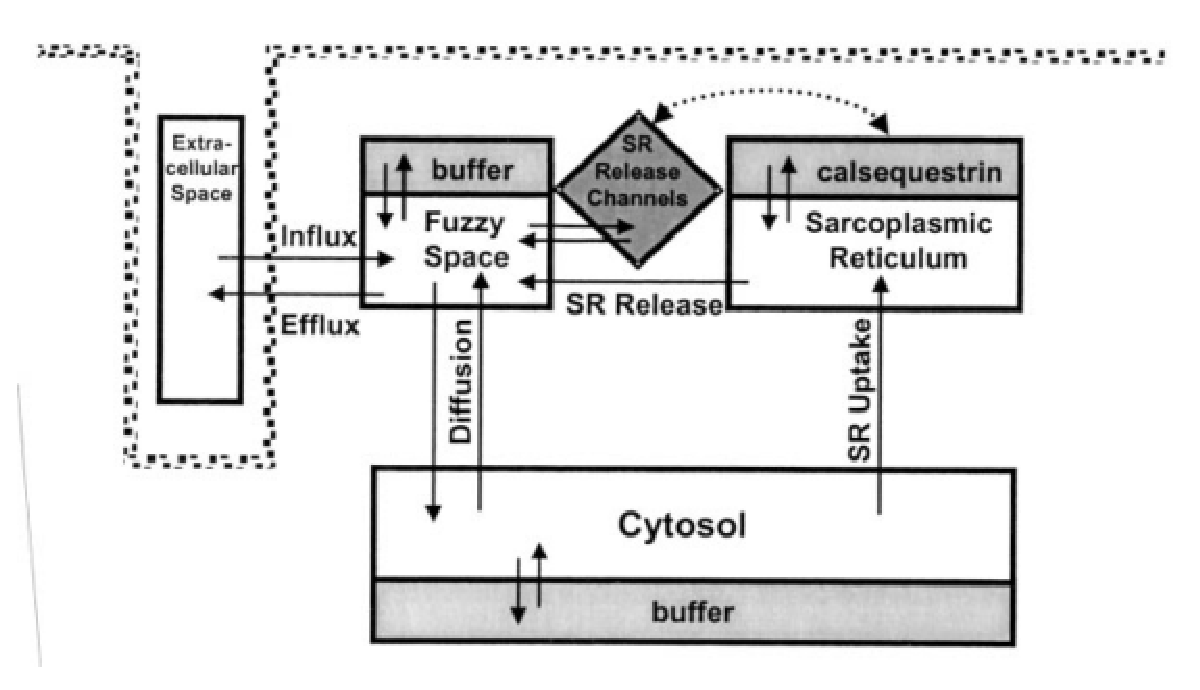
\includegraphics[height=4cm,
    angle=0]{./images/snyder2000_model.eps}}
\caption{Schematic diagram of Snyder}
\label{fig:snyder2000_model}
\end{figure}

\textcolor{red}{The model also incorporate the effect of CSQ to RyR-gating}
(Sect.\ref{sec:RYR_Snyder2000_CSQ}).

\subsection{Mathematical model}

The influx of calcium between the extracellular and subspace was assumed
linearly proportional to the concentration difference
\begin{equation}
J_\ryr  = g_\LCC ([\Ca]_\circ - [\Ca]_\ds)
\end{equation}
with $g_\LCC$ is the collective conductance of LCCs and was opened during 0.02
sec \citep{langer1996} (Sect.\ref{sec:Langer-Peskoff_96}).

Calcium from the fuzzy-space then diffuse to the cytosol
\begin{equation}
J_\ef = v_\ef ([\Ca]_\ds - [\Ca]_\myo)
\end{equation}


\subsubsection{RyR2}

The SRRC is modeled with 4 states, corresponding to 4 binding sites.
\begin{equation}
\ce{Ca^2+ + S_i <=> Ca^2+S_i + Ca^2+ <=> ... <=> (Ca^2+)_nS_i}
\end{equation}
So $n=4$ in our case.

The activation of a single RyR2 was assumed to involve 2 binding steps: one with
high-affinity and then enhance the second $\Ca$-binding. The second binding-step
should be at equilibrium.
\begin{equation}
\frac{d[\text{(Ca)$_{2}$} S_1]}{dt} = k_{on}[\Ca][S_1] -
\frac{(k_{off})^2}{k_{on}[\Ca]} [\text{(Ca)$_2$}S_1]
\end{equation}

The inactivation of a single RyR2 channel was assumed to follow first-order
kinetics with the binding of one $\Ca$ ion to the inactivating site
\citep{fabiato1985scc}.
\begin{equation}
\frac{d[\text{(Ca)$_{2}$} S_2]}{dt} = k_{on,2}[\Ca][S_2] - k_{off,2} [\Ca][S_2]
\end{equation}

So, $[S_1]$ and $[S_2]$ are the concentration of RyR activating sites and RyR
inactivating site. The fraction of RyR channel with calcium-bound at the
activating site ([CaS$_1$]) and the fraction of RyR channel with calcium-bound
at the inactivating site ([CaS$_2$]) can be derived using 2 ODEs
\begin{equation}
\begin{split}
\frac{d[CaS_1]}{dt} &=  \\
\frac{d[CaS_2]}{dt} &=
\end{split}
\end{equation}

The bidirectional interplay was represented as feedback-induced shifts in $\Ca$
binding curves of CSQ and RyRs. These curve shifts are represented in a
simplified form as adjustments in calcium $K_d$ of CSQ and RyRs. The change here
is not incremental over a range of feedback, but implemented as a step change at
the midrange value. Particularly,
\begin{itemize}
  \item  $K_d$ of CSQ is decreased 10x, i.e. $k^+$ jump from $k^{on2}$ to
  $10 \times k^{on2}$, when $[\CaCSQ]$ was below 500$\muM$.
  \item $K_d$ of RyR is increase 20x, when the fraction of opening RyR2s was
  $>0.15$.
\end{itemize}

\subsubsection{NCX}

The NCX was assumed to reside in the fuzzy-space, to extrude calcium from the
fuzzy-space out of the cell. The NCX was modelled using Michaelis-Menten
kinetics
\begin{equation}
J_\ncx = v_\max \frac{[\Ca]_\ds}{K_\max + [\Ca]_ds}
\end{equation}

Here, during LCC opening (0.02 sec), $v_\max=0$. The model is quite simple here.

\subsubsection{SERCA}

SERCA was modelled following second-order reversible Michaelis-Menten kinetics
\begin{equation}
J_\serca = v_{\max, \serca} \frac{\left([\Ca]_\myo^2 -
(\frac{[\Ca]_\nsr}{7000})^2\right)}{\left(K_{m,\serca}^2 + [\Ca]_\myo^2 -
(\frac{[\Ca]_\nsr}{7000})^2\right)}
\end{equation}
Here, the number 7000 was chosen based on the fact that the maximum gradient it
allows is 7000 times different in calcium concentration.

\subsubsection{Calcium buffers}

$\Ca$ buffer in the jSR should not be modelled as instantaneous, but was instead
represented by the ODE form

\begin{equation}
\frac{d[\CaCSQ]}{dt} = k^+ [\Ca]_\jsr ([\CSQ_\tot] - [\CaCSQ]) - k^- [\CaCSQ]
\end{equation}
The bidirectional mechanism was modeled as feedback-induced shift of the $\Ca$
binding curves of CSQ and RyR2s. $[\CSQ]_\tot = 0.008$ mol/L SR water or
800$\muM$ (experiment: 0.005-0.014 mol/L SR water). The dissociation constant
$K_d=638 \muM$ taken from \citep{shannon1997}, with $k^{on}=0.008$
(1/($\muM.s$)) based on \citep{Donoso1995}.

In the case of using Fura-2: [Fura-2] = 50$\muM$ and $K_d=0.2\muM$
\citep{grynkiewicz1985}.

Parameter constants are given in Table 2 (paper).

The accessible water volume of the cell (excluding mitochondria and sarcomeric
protein) was assumed 0.5 L cell water/ 1 L cell total volume, i.e. $V_\cyto=1/2
V_\cell$ \citep{berlin1994iccb, sipido1991}. Total cell volume is 36.8 pL
\citep{delbridge1997}.

The concentration of RyR2s was assumed $1.5\e{-7}$ M, or $1.6\e{6}$ RyR2s per
cell. This is based on the fact that a total cell volume 36.8 pL, and the
fraction of cell that is sarcomeric of 0.6. An individual sarcomeric volume of
1.37 $\mum^3$, it was estimated that there are $\approx 1.6\e{4}$ individual
sarcomeric units (bound by SR and Z lines) per cell. Assuming one fuzzy space
(junctional or diadic cleft) per individual sarcomeric unit, and each fuzzy
space has 100 RyR2s \citep{wibo1991}.

\subsection{Numerical analysis}

The model has 6 ODEs with 33 parameter constants. The ODEs were solved using
fourth-order Runge-Kutta numerical integration method
(Sect.\ref{sec:runge-kutta-method}).

The set of initial values was determined using steady-state assumption (dx/dt =
0), analogous to quiescence and solved using Newton's method for nonlinear
algebraic equations.

\subsection{Data analysis}

To test different conditions, some of the parameters were fixed and allow others
to change dynamically. To compare with experimental data, the calcium transient
was mapped to Fura-2

The model is enough to reproduce graded calcium release (CICR) reponse
\begin{enumerate}
  \item $[\Ca]_\ds$ dependence of the sarcoplasmic reticulum $\Ca$ release
  channel (SRRC) \citep{fabiato1985scc}
  \item refractoriness of SRRC \citep{cheng1996csc}
  \item SR $\Ca$ load dependent of SR $\Ca$ release \citep{bassani1995fsr, gilchrist1992icd}
  \item SR $\Ca$ leak \citep{wier1994lce, bassani1995rdc}
  \item SR $\Ca$ load regulation by leak and uptake \citep{ginsburg1998}
  \item the effect of $\Ca$ trigger duration on SR $\Ca$ release
  \citep{Bers1990}
  \item apparent relationship between sarcoplasmic and sarcoplasmic reticulum
  calcium concentration \citep{shannon1997}
\end{enumerate}

Diastolic calcium leak was estimated to be 0.06mM/s, compared to experimental
meausrement of 0.02 mM/s by \citep{wier1994lce} (similar experimental
conditions: SERCA update and NCX is unaltered). Both are two order of magnitude
higher than the value 0.3 $\muM/s$ measured by \citep{bassani1995a} (where SERCA
is blocked and NCX is stimulated). Using their model, when SERCA is blocked and
NCX is stimulated, the diastolic leak is reduced to 0.24$\muM/s$.


\section{Pandit-\ldots-Demir (adult rat left epi- and endo- myocadial cells)
(2001)}
\label{sec:pandit_2001_rat}

The goal is to study the ionic mechanism that is responsible for the transmural
heterogenity by studying the APD difference between left epi- and endo-
myocardial cells in rat.

\begin{framed}
  AP of cardiac cells from different animals, different heart regions
  have different shapes, durations, and set of ionic
  currents~\citep{fedida1991rva,liu1995cdr,guo1999mbt}.  The rat AP
  has a short AP duration (APD) and relatively dominant transient
  outward current $I_{to}$. APD$_{50}$ in rat ventricular myocytes is
  only 13 ms; while that in guinea pig and canine is about 300
  ms. Due to the short plateau, the shape of the rat ventricular AP
  look like a ``triangular'' shape.

  The human AP has a relative sharp, short peak followed by a slow
  repolarization phase, which takes up 250 ms. In general, APD seems
  to correlated to the heart size or the heart rates of a particular
  species with smaller, faster-beating heart has shorter APD.

  The shape of the underlying currents is more opt to the species and
  region of the heart, rather than the heart size.
\end{framed}

Experiments suggested the prominent role of $I_\to$ ($\Ca$-independent transient
outward current) in distinguishing the two cell regions in most species
(epicardial + endocardial) \citep{Campbell1995,giles1996}, with lower density
and slower recovery from inactivation in endocardial cells \citep{clark1993,
shimoni1995}.

Also, there are some evidences of transmural gradient of $\Na$ currents with
higher density in endocardium \citep{ashamalla2001}. The disruption of this
transmural gradient leads to altered rates of repolarization across the wall,
which is associated with the generatin of arrhythmias. The larger density of
$I_\na$ results a faster upstroke $dV/dt_\max$ that in combined with smaller
amplitude of $I_\to$ produces a larger peak. The longer APD in endocardial is
the result of enhanced amplitude of the $I_\ds$ and larger influx of calcium via
$I_\ca$.

To confirm the above experimental observation, \citep{pandit2001} introduced a
model for epicardial (at the apex) and endocardial (at the base) myocytes
isolated from adult rat left ventricular myocytes. Compared to epicardial
myocytes, endocardial myocytes in healthy adult rat have longer APD
\citep{clark1993}, more prominent rate-dependent effects on APD
\citep{shimoni1995}, and a larger peak overshoot \citep{shipsey1997,volk1999}.

\textcolor{red}{The rat cell volume they used is too small for adult rat
ventricle cell: 16pL} (should be around 36pL), which gives whole cell
capacitance 100pL. This data is based on \citep{Bouchard1995}.
The capacitance-to-volume ratio is 6.25 pF/pL, which a little low compared with
an old measurement 6.76$\pm$ 0.62 pL \citep{satoh1996svr}.

\subsection{Hypothesis}


The model is based on LR-2 model, and the classical formulation of
Hodgkin-Huxley \citep{hodgkin1952ap} for ionic channels. Both models for
endocardial and epicardial cells used the same formulation, with some
difference in parameters.

\begin{figure}[hbt]
  \centerline{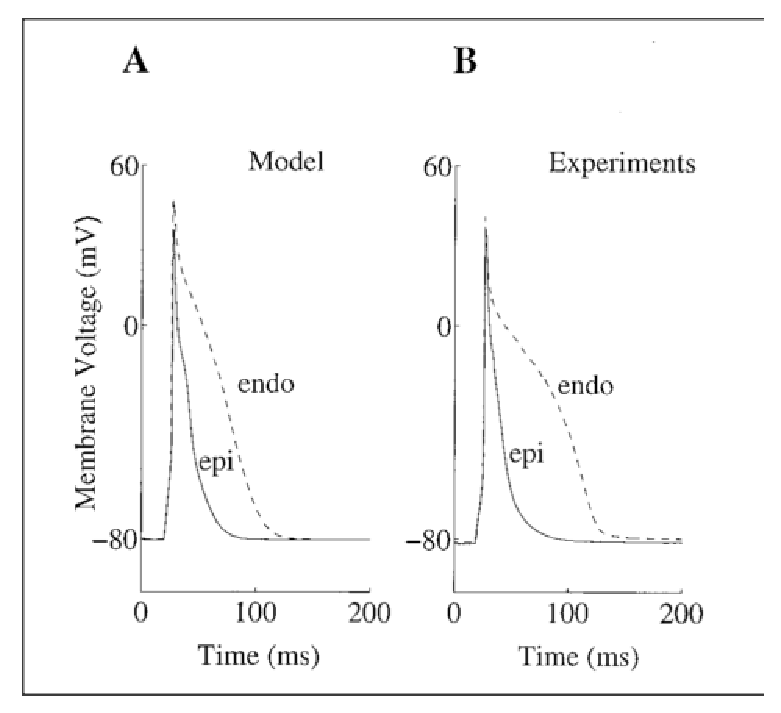
\includegraphics[height=5cm]{./images/Pandit_AP_epi_endo.eps}}
\caption{(A) AP in model and (B) AP from experiment}
\label{fig:Pandit_AP}
\end{figure}

\subsection{Mathematical model}

\subsubsection{$I_\Na$ currents}

The Hodgkin-Huxley formulation for $I_\Na$ is used with fast activation variable
($m^3$), one fast inactivation gate ($h$) and one slow inactivation gate ($j$)
(Sect.\ref{sec:Ina_Beeler-Reuter_1977}).

The steady-state activation/inactivation curve is based on patch-clamp
data \citep{lee1999}. The basic kinetics characteristics of $I_\Na$ are similar
in ventricular myocytes across species, so the time constants were adapted from guinea pig
ventricular myocytes \citep{luo1994dmc_a} scaled to room temperature.




\subsection{Data analysis}

The result supported the hypothesis that
\begin{enumerate}
  \item faster upstroke ($(dV_m/dt)_\max$) determined by larger density of
  $\Na$ channels ($I_\Na$)
  \item longer APD determined by the smaller density and slower reactivation
  kienetics of $\Ca$-independent transient outward potassium current $I_\to$.
\end{enumerate}

\section{Puglisi-Bers (2001) - LabHEART (rabbit)}

\citep{puglisi2001} introduced an interactive software for rabbit ventricular
myocyte. The software aimed to provide a user-friendly interface (using
mouse-click on an icon to modify parameters's values or protocols). Features:
\begin{enumerate}
  \item switching between Voltage clamp and Current clamp (AP)
  \item On-line manipulation of key parameters to change the original
  formulation, i.e. they can be changed while the simulation is running.
  \item reproduce normal rabbit ventricular myocyte currents, Ca transients, and
  AP with standard plots as built-in features (I-V curves, steady-state
  activation and inactivation curves)
\end{enumerate}

\subsection{Mathematical model}

To reproduce AP data from rabbit ventricular myocytes, parameters's values are
based on Luo-Rudy II, e.g. SERCA, $I_\Nab$, Ca release, buffering; with some
modifications
\begin{enumerate}
  \item $\Na$ current: $g_\na=8$mS/$\muF$ (from value 16)
  \item $I_\to$ :
\end{enumerate}

\subsection{Analysis}

To simulate data from heart failure (HF) which showed a decrease in $\Ca$
transient amplitude and increased AP duration, they kept calcium current
density, but changed
\begin{enumerate}
  \item reduce transient outward $I_\to$: no effect to threshold

  \item reduce inward rectifying curent $I_{\k1}$: showed the threshold for a
  triggered AP reduced from 0.8$\muM$ to 0.6$\muM$.
  \item enhanced NCX: showed the threshold $[\Ca]_\myo$ for a triggered
  AP reduced from 0.8$\muM$ to 0.54$\muM$ (as more/faster calcium extruded out
  of the cell).
  \item reduce SERCA
\end{enumerate}
Combining changes in $I_{\k1}$ and NCX reduced the threshold to 0.38$\muM$. The
authors suggested that the altering in $I_{\k1}$ and NCX play an
approximately equally role to triggered AP that contribute to
non-reentrant ventricular tachycardia in HF.






\section{Fox-McHarg-Gilmour model (2002) - canine with alternans}
\label{sec:fox-mcharg-gilmour}

Winslow {\it et al.} model (Sect.~\ref{sec:winslow-et-al}) for canine
ventricular myocyte and LRd (or LR2) (Sect.~\ref{sec:luo-rudy-phase-2}) for
guinea pig didn't produce sustained alternans at rapid pacing rates. Chudin {\it
et al.} model (Sect.\ref{sec:chudin-et-al} a modification of LR-2 model) though
can generate electrical alternans, lack the formulation of repolarizing $\K$
current (rapid and slow component of DR:$I_\Kr,I_\Ks$, and transient outward
current $I_{K,to}$).

What Fox-McHarg-Gulmour did was to build a model combining Winslow
{\it et al.}, Chudin {\it et al.}, identify the ionic currents
that exhibit stable electrical alternans, and then modify these
currents to see when they eliminate alternans.

\subsection{Hypothesis analysis}
\label{sec:hypothesis-analysis-14}

Even though decreasing $I_\ca$, either experimentally and simulation,
shown that it can eliminate alternans, this is not useful clinically
as it decreases $\Ca$ transient, thereby reducing contractile force.

A potential approach, from the model is to increase $I_\Kr,I_\Ks$
and $I_{K1}$ as they decrease APD. That may explain why class II
antiarrhythmic drugs, which are designed to block $\K$ currents, have
been shown to be proarrhythmic~\citep{Peters2000}.

For most parts of the model, it's similar to Winslow {\it et al.}
model (Sect.~\ref{sec:winslow-et-al}). The major differences
\begin{enumerate}
\item L-type channel: they use Hodgkin-Huxley based formula (from LR2
  model), rather than Markov-chain model.
\end{enumerate}

For calcium handling, the modified version of~\citep{chudin1999icd}
was used. They neglected the spontaneous release of calcium from SR
via CICR mechanism, i.e. NSR and JSR is combined as a single
compartment. Apart from that, effect of buffering from calmodulin in
the cytoplasm and calsequestrin (CSQ) in the SR were added.

\subsection{Mathematical model}
\label{sec:mathematical-models}

\subsection{-- Ion concentrations}
%\label{sec:ion-concentrations}

\begin{enumerate}
\item $[\Ca]_i$: myoplasmic calcium concentration
\begin{equation}
  \label{eq:1065}
  \frac{d[\Ca]_i}{dt} = \beta_i (J_\rel+J_\leak - J_\up - J_{\ca,\sr})
\end{equation}
with
\begin{equation}
  \label{eq:1066}
  J_{\ca,\sr} = \frac{A_{cap}\Csc}{z_\ca FV_\myo} \left( I_\ca+I_\Cab
  + I_\pmca - 2I_\naca \right)
\end{equation}
and buffering
\begin{equation}
  \label{eq:1068}
  \beta_i = \frac{1}{1+[\CMDN]_{tot} \frac{K^\CMDN_m}{K^\CMDN_m+([\Ca]_i)^2}}
\end{equation}

\item $[\Ca]_\sr$: sarcolemmal calcium concentration
\begin{equation}
  \label{eq:1067}
  \frac{d[\Ca]_\sr}{dt} = \beta_\sr \left( J_\up -J_\leak -J_\rel
  \right) \frac{V_\myo}{V_\sr}
\end{equation}
and buffering
\begin{equation}
  \label{eq:1069}
  \beta_i = \frac{1}{1+[\CSQN]_{tot} \frac{K^\CSQN_m}{K^\CSQN_m+([\Ca]_i)^2}}
\end{equation}
\end{enumerate}



\subsection{Analysis}
\label{sec:analysis-15}


\subsection{Numerical methods}
%\label{sec:numerical-methods-1}

A C program runs on Macintosh G3 and G4. Numerical integration scheme
is similar to that used in LR1 and ~\citep{rush1978pas}.

Time steps were chosen
\begin{itemize}
\item small enough so that the change in voltage and calcium
  concentration remain below the maximum values $\Delta
  V_\max$=0.8mV,$\Delta \ca_\max$=1.067$\times 10^{-2}\muM$.

\item increase so that the change in voltage and calcium concentration
  remain above the minimum values $\Delta V_\min$=0.2mV,$\Delta
  \ca_\min$=2.67$\times 10^{-3}\muM$.
\end{itemize}

The ODEs were solved using fourth-order Runge-Kutta method
(Sect.\ref{sec:runge-kutta-method}).
The errors were normalized as described in JRW model
(Sect.~\ref{sec:jafri-rice-winslow}) with maximum error $10^{-6}$,
minimum time step $0.005$ms, and maximum time step 0.5ms. During
stimulation $I_\stim$ time step is fixed at 0.005ms.

To further increase computational speed, look up tables are used to
avoid recalculating exponential and other expensive functions.

\section{Bernus-\ldots-Panfilov (2002) (human)}

\citep{bernus2002} is the simplification of \citep{priebe1998}
(Sect.\ref{sec:priebe-beukelmann_1998}). This is the second models for human
ventricular myocytes. The drawbacks of the two models are discussed in
Sect.\ref{sec:tenTusscher2004_human}.


\section{Padmala-Demir (2003) - rat}

~\citep{padmala2003} modified the model (Sect.\ref{sec:pandit_2001_rat}) by introducing the
new formulation of $I_{K1}$ (inwardly rectifying K current) which
\begin{equation}
  \label{eq:1409}
  I_{K1} = g_{K1} \sqrt{[\K]_o} \frac{V_m-E_\k-1.8}{1+\exp(1.81\frac{V_m-E_\k}{RT/F})}
\end{equation}
where $g_{K1}=11.93$ nS, T=295K, R=8,314 mJ/(mol.K); and F=64,487
C/mol. This model was then used to study Spontaneously Hypertensive
Rat (HSR) in ventricular myocyte.


\section{Shiferaw-\ldots-Karma (2003)}
\label{sec:shiferaw-et-al}

~\citep{shiferaw2003} presented a new model of EC coupling with the release from
SR is the summation of discrete events, $\Ca$ sparks. However, the model for
$\Ca$ sparks is relatively unrealistic. At first, it assumes $\Ca$ sparks
depends only on lumincal $\Ca$, not subspace calcium $[\Ca]_\ds$. Secondly, the
spark duration is modeled as a single exponential decay function. Essentially,
the stochastic gating of RyR and LCC were neglected. Instead, they model the
stochastic recruitment of sparks.

The SR is a spatially diffuse network composed of two pars:
the network SR (NSR) and the junctional SR (JSR). NSR is the meshwork of tubules
that enwraps the myofilaments. JSR is the flattened elliptical sacs branched out
from the NSR.

\subsection{Hypothesis analysis}
\label{sec:shiferaw2003_hyp_anal}

The SR is assumed to composed of $N_\jsr$ identical JSR compartments, each with
volume $v_\jsr$. The NSR has volume $v_\nsr$. Then the total SR volume is
\begin{equation}
\label{eq:shiferaw2003_1}
v_\sr = v_\nsr + N_\jsr \times v_\jsr
\end{equation}

Calcium concentrations:
\begin{enumerate}
  \item at each JSR: $c^k_\jsr$
  \item at NSR: $c_\nsr$
  \item the average total calcium concentration in the SR $c_\sr$
  \begin{equation}
  \label{eq:shiferaw2003_2}
  c_j = \frac{1}{v_\sr}\left[ v_\nsr\times c_\nsr +
  \sum^{N_\jsr}_{k=1} v_jsr\times c^k_\jsr \right]
  \end{equation}
  \item the average of calcium from unrecruited dyadic subspace: $c'_j$

  \item submembrane space: $c_s$ with volume $v_s$ (NOTE: $v_s \ll v_i$ then
  the concentration change in the submembrane space are much larger and faster
  than those in bulk myoplasm). Here they use $v_i/v_s \sim 10$.

  NOTE: The reason of using submembrane space is that $I_\ncx$, due to its close
  proximity to dyadic space, sense a calcium concentration different from that
  in the bulk myoplasm. It means that when calcium change more and faster, NCX
  model serves as a more efficient calcium efflux mechanism.

  \item the bulk myoplasm: $c_i$ with volume $v_i$

  \item the dyadic subspace: $c^k_\ds$ (with $k=1\ldots N_\jsr$).
\end{enumerate}


\begin{figure}[hbt]
  \centerline{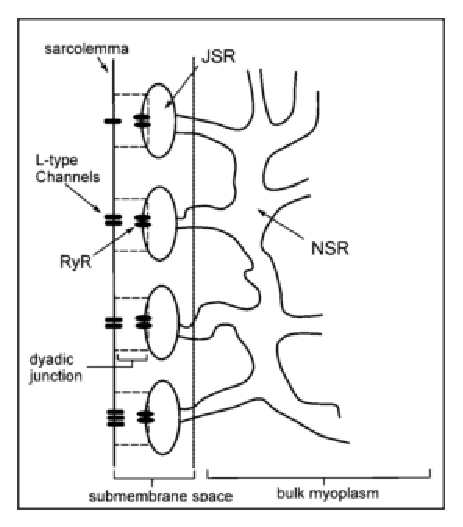
\includegraphics[height=5cm,
    angle=0]{./images/shiferaw_2003.eps}}
  \caption{Intracellular spaces in Shiferaw et al. model}
  \label{fig:smith_spark}
\end{figure}

\subsubsection{LCC current}

LCC is modeled using a simple Hodgkin-Huxley formulation
\begin{equation}
I_\ca = MP_o i_\ca
\end{equation}
with $i_\ca$ is single channel current, $M$ is total number of LCCs in the cell,
$P_o$ is time-dependent open probability of a single channel.
\begin{equation}
P_o = d_\infty .f.q
\end{equation}
with $d_\infty$ is instantaneous $V_m$-dependent activation gate, $d$ is slow
$V_m$-dependent inactivation gate, and $q$ is $\Ca$-induced inactivation.

\subsubsection{Spark rate and duration}

The relationship between the spark occurrence, i.e. the number of sparks N(t),
and the calcium current $I_\ca$ is defined based on the rate of spark
recruitment $dN(t)/dt$. Based on experimental data \citep{collier1999}, under
the physiological condition and for a given depolarized potential, $dN(t)/dt
\approx I_\ca(t)$ (linear relation).
\begin{equation}
\label{eq:shiferaw2003_03}
\frac{dN(t)}{dt} = gI_\ca(t) A(c'_j(t))
\end{equation}
with $A(c'_j)$ is a function that tell JSR $\Ca$ load dependence (i.e. average
calcium concentration within unrecruited JSR compartment), $g$ is a
proportionality constant.

Here, the spark dynamics is assumed to depend upon JSR $\Ca$ only ($c^k_jsr$),
than the concentration of local dyadic subspace calcium $c^k_\ds$
(\textcolor{red}{this is a flaw in the model as RyR gating is} $[\Ca]_\ds$
dependent).
Another assumption is that each spark at each release site, once recruited, has
a constant lifetime $\tau^k_r$. Experiments shown spark have a well defined
lifetime arount 10-30ms \citep{niggli1999}.
So, they modeled the termination of SR $\Ca$ release as an exponentially decay
function of time, from the initial peak value, using a time constant comparable
to the observed spark lifetime.
\begin{equation}
I^k_\text{spark}(t,t') = J^k(c^k_\jsr(t')) \exp(-\frac{t-t'}{\tau^k_r})
\end{equation}
with $t'$ is the time spark activated; $J^k(\cdot)$ is the flux across
RyRs whose amplitude is a function of JSR $\Ca$ load only. \textcolor{red}{The
stochastic gating of RyRs thus has not been incorporated in the model}.

Using ensemble approach, they assume that the ensemble spark fluxes has a
well-defined property, i.e. $c^k_\jsr(t')=c'_j(t')$. It means that at the time
$t'$, when the spark is being recruited, the calcium at the dyadic subuspace is
not depleted, and the concentration at this time can be roughly assumed to be
approxiamted by the average concentration in unrecruited JSR compartments
$c'_j(t')$. So, the ensemble spark is now denoted by $I_\text{spark}(t,t')$ with
\begin{equation}
I_\text{spark}(t,t') = J(c'_j(t')) \exp(-\frac{t-t'}{\tau_r})
\end{equation}


\subsection{Mathematical analysis}
\label{sec:shiferaw2003_math}

\textcolor{red}{Currents}:

\begin{enumerate}
  \item Na/Ca exchange (NCX): use Luo-Rudy II.
  \item Na current $I_\na$: a phenomenological rate-depent of $I_\na$ has been
  developed, i.e. $[\Na]_i$ is an increasing function of pacing rate.

  NOTE: When pacing from 0.5Hz to 3Hz, twitch shortening increase 34\%. However,
  when $I_\na$ is blocked (using tetrodotoxin), the twitch shortening increase
  only 8\%. So, rate-dependent change in $[\Na]_i$ may have certain effect on
  $[\Ca]_i$
  \item $\Ca$ uptake via SERCA is modeled simple using Hill equation
\end{enumerate}

\textcolor{red}{Fluxes}:
\begin{enumerate}
  \item The flux from submembrane space to bulk myoplasm $I_d$
  \begin{equation}
  I_d = (c_s-c_i)/\tau_s
  \end{equation}
  with the ralaxation time constant $\tau_s$ in the range 5-10ms.
\end{enumerate}


\textcolor{red}{Buffering}:
\begin{enumerate}
  \item In myoplasm: troponin C, SR and calmodulin (Cd) sites. The binding to SR
  and calmodulin sites are assumed fast, i.e. instantaneous with the buffering
  factor $\beta(c_i)$
  \begin{equation}
  \beta(c_i) = \left[ 1 + \frac{[B]^T_\sr K_\sr}{(c_i + K_\sr)^2} +
  \frac{[B]^T_\CaM K_\CaM}{(c_i + K_\CaM)^2}  \right]^{-1}
  \label{eq:shiferaw2003_05}
  \end{equation}

  \item In the submembrane space: like that in myoplasm, $\beta(c_s)$. The
  fomular is similar as eq.\ref{eq:shiferaw2003_05}, except $c_i$ is replaced by
  $c_s$.
\end{enumerate}


\subsection{Data analysis}
\label{sec:shiferaw_dataanalysis}

At high pacing rates, the model exhibit sustained calcium alternans.


\section{ten Tusscher-Noble-Noble-Panfilov (2004) (human) }
\label{sec:tenTusscher2004_human}

The two previous models for human cardiac myocytes \citep{priebe1998,
bernus2002} have some drawbacks: (1) parameters are derived from animal data
(not human), (2) APD $\sim $360ms is much longer than the value recorded in
tissue ($\sim 270$ms) \citep{li1998}. So, \citep{tenTusscher2004} derived a new
model using new experimental data \citep{morgan1992}, which is supposed to be
more accurated to the dynamics of human ventricular myocyte and computational
efficient for large-scale spatial simulation of reentrant phenomena.

The model includes: $I_\na$, $I_{\to}$, $I_{\Kr}$ (rapid component of delayed
rectifier), $I_\Ks$, $I_{K1}$ (inward rectifier $\K$ current), $I_\ca$.


Calcium dynamics being used in the model is simple, just to reproduce the
realistic calcium transient.

\subsection{Hypothesis analysis}

\subsection{Data analysis}

The model was used to generate different APD and AP shapes according to
different regions (endo-, epi- and mid-myocardial regions of the ventricles),
and rate dependencies.

\section{Bondarenko-...-Rasmusson model (2004) - mouse model}
\label{sec:bond-rasm}

In this paper, the authors use Markov models to represent the
molecular structure and functions of all ion
channels for mouse ventricular myocytes at two
different regions: apex (relatively long AP) and septum
~\citep{bondarenko2004cma}. However, the model is ``common-pool''.

All parameters are adjusted at room temperature (25$^\circ$C or 298K).

Another model by the group is mentioned in \citep{bondarenko2004mgc}.
Each CRU has 4 L-type $\Ca$ channels (DHPR).


% \section{Probabilistic approach}
% \label{sec:prob-appr}


\section{Shannon-\ldots-Bers (2004) rabbit}
\label{sec:shannon_2004_rabbit}

\citep{shannon2004} proposed a common-pool model for rabbit ventricular
myocyte, Fig.\ref{fig:shannon04_rabbit}. The model examined the dynamics of both
$[\Ca]_i$ and $[\Na]_i$. The dynamics of $V_m$ is based on Luo-Rudy model
\citep{luo1994dmc_a,luo1994dmc_b} with modified parameters to work for rabbit
ventricular myocyte at body temperature (37$^\circ$C).


\begin{figure}[hbt]
  \centerline{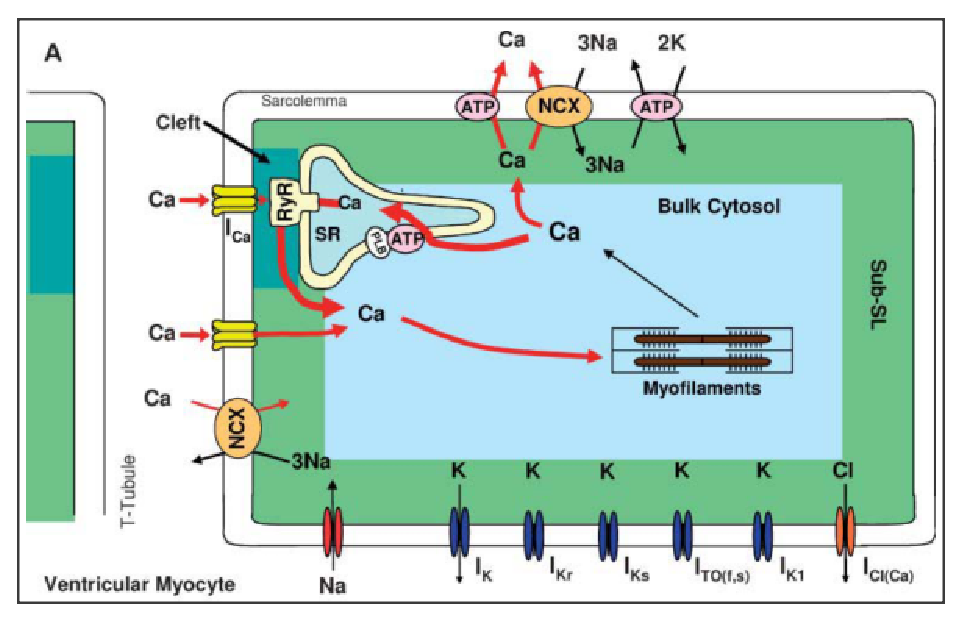
\includegraphics[height=5cm,
    angle=0]{./images/shannon_04_rabbit.eps}}
  \caption{Schematic diagram of rabbit ventricular myocyte}
  \label{fig:shannon04_rabbit}
\end{figure}

Limitation: Dyes like Indo-1 and Fluo-3 are not incorporated in the model for
simulation results; except when they were added to test the effect on calcium
transient. [QUESTION: Other than reducing peak, do they also affect to other
properties of calcium dynamics?]


\subsection{Hypothetical analysis}

\subsubsection{Volumes}

It's assumed that calcium efflux from the subspace flow into a sub-sarcolemmal
membrane (SL) region which cause a higher $\Ca$ concentration that that in bulk
myoplasm. This higher $[\Ca]$ is detected by NCX and $\Ca$-dependent $\Cl$
channels. Thus, a subsarcolemmal compartment is incorporated into the model.

The cell volume is 33 pL with 4 compartmental components
\begin{enumerate}
  \item SR volume is 3.5\% \citep{page1971} (rat data);
  \item the subspace volume (junctional cleft volume) is assumed to be a disk of
  radius 160 nm and 15-nm deep. So the volume is 0.077\% (based on the
  assumption that 11\% of the SL is junctional and the cleft is 15-nm deep)
  \citep{page1979, soeller1997}. However, the accessible volume is reduced
  one-third occupied by proteins. So the effective volume is 0.051\%.

  \item subsarcolemmal volume is 2\% (based on the assumption that 89\% of the
  membrane is non-junctional SL and the region is 45-nm deep).
  \item bulk cytosolic volume is 65\%
\end{enumerate}
The remaining volume was assumed mitochondria which is not
considered explicitly in the model \citep{page1971}. The number of subspace,
when spaced evenly 1.2$\mum$ apart from the center to center over the entire
cell membrane area of 15,000$\mum^2$ (or 4.58pF/pL, given 1$\muF$/cm$^2$), it
gives the number of release site as 20,000.


At resting level $[\Ca]_\myo=100$nM, the unidirectional forward flux (uptake)
through SERCA pump is estimated about 25$\mu$mol/L cyt./sec. Previous
measurement the leak out of SR via RyRs is 4-15$\muM$/s \citep{shannon2002,
lukyanenko2001}. It was suggested that the residual efflux should be going
through the backflux of SERCA pump. Even though this is physiologically
incorrect, as it accounts for more than 50\% of the counterflux and this
requires a lot of ATP for SERCA pump, the authors used the backflux SERCA model
developed by \citep{shannon2000rms} [IMPORTANT: Later on, the concept of
'invisible' leak that account these leak via RyR stochastic opening channels].


\subsubsection{$\Na$ current}

$\Na$ buffers were located only in junction and SL compartment, to incorporate
the effect of $\Na$-dependent NCX. The buffers are modeled as rapid binding
molecules with standard Hill equation.


\subsubsection{Calcium currents}

Calcium buffers were incorporated in each compartment (Table 7 in the paper)
SR $\Ca$ buffers (primarily calsequestrin CSQ) were modeled as rapid binding
molecules. Parameters from \citep{shannon1997, shannon2000pfs, shannon2000rms}.

\begin{enumerate}
  \item Cytosol: TroponinC (Bmax=70$\mu$mol/L cyt.; Kd=0.6$\muM$, koff=19.6,
  kon=32.7$(\muM.s)^{-1}$); Troponin C Ca-Mg (Ca); Troponin C Ca-Mg (Mg);
  Calmodulin; Myosin (Ca); Myosin (Mg); SR-buffer

  \item SL: SL-protein, SLhigh-protein, Indo-1 buffer, Fluo-3 buffer
  \item Junction: SL-protein, SLhigh-protein, Indo-1 protein, Fluo-3 protein
  \item SR: Calsequestrin
\end{enumerate}
In most of the simulation, dyes were not incorporated. However, for testing
purpose, dyes were added (at concentration 25$\muM$) and they reduced peak $\Ca$
transients by 20\%, and slowed the rate of steady-state $\Ca$ transient.


\subsection{Numerical analysis}

The model was written in C language on Dell Precision 3500 Pentium 4 2.4GHz with
512MB RAM running Linux RedHat 9.0.
The ODEs were solved using CVODE
package\footnote{\url{http://www.netlib.org/ode/index.html}}.


\section{Iyer-Mazhari-Winslow (2004) - human left ventricular epicardial}
\label{sec:Iyer-Winslow2004}

\citep{iyer2004} created a model for human left-ventricular epicardial myocyte,
using experimental data from recombinant human single channels and whole-cell
recording of human left-ventricular subepicardium. Data are represented at
physiological temperature.

Different ion concentrations ($\Ca, \Na, \K$) are examined in the model.

\subsection{Hypothesis analysis}

The model includes: $I_\na$, $I_{\to}$, $I_{\Kr}$ (rapid component of delayed
rectifier), $I_\ca$.

$\Na$ channels is modeled using continuous-time Markov chain model
\citep{irvine1999}, rather than using the Hodgkin-Huxley-based approach. The
model state transition rates are explicit functions of {\it enthalphy}, {\it
entropy}, $V_m$, and temperature (Sect.\ref{sec:Ina_Iyer2004}).



\subsection{Mathematical model}

Data:
\begin{enumerate}
  \item  Total membrane capacitance $A_\cap=153.4$pF.

  \item Volumes: cytosol 25.84pL,
junctional SR = 0.16pL, network SR = 2.1pL, dyadic subspace = 1.2$\times
10^{-3}$pL (=285*285*14.7nm).

  \item Concentration: $[\Ca]_o=2$mM, $[\Ca]_i=0.1\muM$, $[\Ca]_nsr=1.0$mM
  \item Transfer rate: $\tau_\ef = 7\times 10^{-7}$ s,
  $\tau_\rf=0.003$s
\end{enumerate}


\subsection{Numerical method}

Methods to extrapolate $I_\na$ to 33$^\circ$C are given below.

\subsection{Data analysis}

The simulated $I_\na$ channel current is compared with expiremental data from
recombinant human hH$_1$ channels. Here, the data on activation (time-to-peak),
inactivation, and recovery from inactivation largely fall within the
experimental error bars (Fig.1 in paper). The results were collected using
voltage-clamp in the range -50mV to +30mV (holding potential is -150mV), and
time-step duration is 24ms (temperature 33$^\circ$C). Here, the decay was fitted
with a sum of two weighted exponential functions: fast $\tau_\text{fast}$ and
slow $\tau_\text{slow}$.

The model is suggested to reproduce a wide range of behaviors observed
experimentally: AP morphology, ionic currents, $[\Ca]_i$ transients, frequency
dependence of APD, extrasystolic restitution/post-extrasystolic potentiation.



% The model can reproduce frequency-dependence of APD, $\Ca$-frequency relations,
% and extra-systolic restitution/post-extrasystolic potentiation.


\section{Faber-Rudy (2007) - CPVT guinea pig}
\label{sec:Faber_Rudy_07}

They exploited the possible effect of muation CASQ2$^{D307H}$, and exploit SOICR
as a possible mechanism for CPVT. As CPVT occurs under stress or exercise, they
modeled this by making change to LCC ($I_\CaL$) and other currents, reflecting
the application of saturating isoproterenol (ISO $\ge 0.1\muM$) in experiments.

The model is developed based on LRd model \citep{luo1994dmc_b}
(Sect.\ref{sec:luo-rudy-phase-2}). LCC is modeled with 14-state (in 2 modes: Ca
and V), and when ISO is applied it  may swith to a new mode (mode0)
\citep{faber2007DHPR}.


\section{Grandi-\ldots-Bers (2010) - human}
\label{sec:Grandi-Bers_09}

\citep{grandi2010}


%%% Local Variables: 
%%% mode: latex
%%% TeX-master: "mainfile"
%%% End: 
